\chapter{\texorpdfstring{Searches for New Physics in $\tau^+\tau^-$ Final States}{Search for new physics in tautau final states}}
\label{sec:bsm_H_to_tau_tau_analysis}
 
The $\tau^+\tau^-$ final states are a powerful tool to search for new physics at collider experiments. 
As the heaviest lepton, they are sensitive to resonant production of new neutral particles where the couplings have mass hierarchy.
They are also sensitive to non-resonant effects from new physics mediators. 
This chapter will detail the searches for two such areas of new physics: additional Higgs bosons and vector leptoquarks.
These searches are split up into three sections: 
\begin{enumerate}[i)]
  \item A model independent search for single narrow spin-0 resonance, $\phi$, produced via gluon fusion (gg$\phi$) or in association with a bottom quark (bb$\phi$). The SM Higgs boson is treated as a background. The Yukawa couplings that contribute to the gluon fusion loop are set to SM values.
   \item A search for the MSSM Higgs sector, in a number of benchmark scenarios. The benchmark scenarios are defined in Section~\ref{sec:additional_higgs_bosons}. The production of SM Higgs boson is also used to constrain the available phase space.
  \item A search for the t-channel exchange of a $U_{1}$ vector leptoquark. Two scenarios are taken, based of the best fit to the b anomalies. These scenarios are detailed in Section~\ref{sec:vlq}.
\end{enumerate}

These searches are performed with the full run-2 dataset ($138 \sifb$) collected by the CMS experiment. 
The search for additional Higgs bosons had previously been performed with data collected in 2016 ($39 \sifb$) and results were consistent with the SM background prediction.
 
\section{Signal Modelling} 
 
\subsection{Additional Higgs Bosons} 
\label{sec:additional_higgs_bosons} 
 
Extended Higgs sectors, such as that of the MSSM, can be probed by direct searches for the additional bosons and further precise measurements of the Standard Model Higgs boson. 
This search for an extended Higgs sector is motivated by Type II 2HDMs, such as the MSSM.
In these models $\tan\beta$ enhances couplings of additional Higgs bosons to bottom-like quarks and leptons, whilst top-like couplings are suppressed.
This narrows down the most important production modes of the Higgs boson into two categories: Gluon fusion and production in association with a bottom quark.
Examples of these are shown in Figure~\ref{fig:mssm_feynamn}.

\begin{figure}[H]
\centering
\begin{subfigure}[b]{0.3\textwidth}
\begin{tikzpicture}[scale=2]
  \begin{feynman}
    \vertex [label=left:$g$] (a1) at (0,0);
    \vertex [label=left:$g$] (a2) at (0,1);
    \vertex (b1) at (1,0);
    \vertex (b2) at (1,1);
    \vertex (c) at (1.7,0.5);
    \vertex [label=right:$h/H/A$] (d) at (2.7,0.5);

    \diagram* {
      (a1) -- [gluon] (b1),
      (a2) -- [gluon] (b2),
      (b2) -- [fermion] (b1),
      (c) -- [fermion] (b2),
      (b1) -- [fermion] (c),
      (c) -- [scalar] (d),
    };
  \end{feynman}
\end{tikzpicture}
\caption{}
\end{subfigure}


\begin{subfigure}[b]{0.3\textwidth}
\begin{tikzpicture}[scale=2]
  \begin{feynman}
    \vertex [label=left:$g$] (a1) at (0,0);
    \vertex [label=left:$g$] (a2) at (0,1);
    \vertex (b1) at (1,0);
    \vertex (b2) at (1,0.5);
    \vertex (b3) at (1,1);
    \vertex [label=right:$b$] (c1) at (2,0);
    \vertex [label=right:$h/H/A$] (c2) at (2,0.5);
    \vertex [label=right:$\bar{b}$] (c3) at (2,1);
    \diagram* {
      (a1) -- [gluon] (b1),
      (a2) -- [gluon] (b3),
      (b3) -- [fermion] (b2),
      (b2) -- [fermion] (b1),
      (c3) -- [fermion] (b3),
      (b1) -- [fermion] (c1),
      (b2) -- [scalar] (c2),
    };
  \end{feynman}
\end{tikzpicture}
\caption{}
\end{subfigure}
\hspace{2cm}
\begin{subfigure}[b]{0.3\textwidth}
\begin{tikzpicture}[scale=2]
  \begin{feynman}
    \vertex [label=left:$g$] (a1) at (0,0);
    \vertex [label=left:$b$] (a2) at (0,1);
    \vertex (b) at (0.7,0.5);
    \vertex (c) at (1.4,0.5);
    \vertex [label=right:$b$] (d1) at (2.1,0);
    \vertex [label=right:$h/H/A$] (d2) at (2.1,1);
    \diagram* {
      (a1) -- [gluon] (b),
      (a2) -- [fermion] (b),
      (b) -- [fermion] (c),
      (c) -- [fermion] (d1),
      (c) -- [scalar] (d2),
    };
  \end{feynman}
\end{tikzpicture}
\caption{}
\end{subfigure}
\caption{Diagram (a) shows the production of neutral Higgs bosons from gluon fusion. The dominant loop contributions to this diagrams are from top-only, bottom-only and top-bottom interference. Diagrams (b) and (c) show production in association with b quarks.}
\label{fig:mssm_feynamn}
\end{figure}

With the $\tan\beta$ enhancement, the decays of additional Higgs bosons to tau leptons and bottom quarks are most likely.
Tau leptons are identified with a higher purity than bottom quarks a the CMS detector.
It is also easier to separate $\tau^{+}\tau^{-}$ from the large QCD multijet background produced from the high energy proton-proton collisions.
This hypothesis was tested with the 2016 dataset and although no deviations were observed, the strongest limits on the MSSM phase space was placed by the $\tau^+\tau^-$ final states. \\

For this analysis, the production of additional Higgs bosons over a mass range of 60 GeV to 3.5 TeV are generated.
Gluon fusion is simulated at NLO precision using the 2HDM implementation of POWHEG 2.0.
The kinematic properties are highly dependent on the contributions to the loop, which vary dependent on the specific signal model.
To account for the different loop contributions at the NLO plus parton shower prediction, weights based off the $\pT$ spectra are calculated to split the contributions from the t quark only, b quark only, and tb-interference.
Once individual templates have been determined for each contribution to the loop, the 2HDM samples can be scaled to the correct specific MSSM scenario prediction by the following formula.

\begin{equation}
\begin{aligned}
\frac{d\sigma_{\text{MSSM}}}{d\pT} & = \left(\frac{Y_{t,\text{MSSM}}}{Y_{t,\text{2HDM}}}\right)^{2}\frac{d\sigma^{t}_{\text{2HDM}}}{d\pT}(Q_{t}) + \left(\frac{Y_{b,\text{MSSM}}}{Y_{b,\text{2HDM}}}\right)^{2}\frac{d\sigma^{b}_{\text{2HDM}}}{d\pT}(Q_{b}) + \nonumber \\
& \left(\frac{Y_{t,\text{MSSM}}}{Y_{t,\text{2HDM}}}\frac{Y_{b,\text{MSSM}}}{Y_{b,\text{2HDM}}}\right) \left\{ \frac{d\sigma^{t+b}_{\text{2HDM}}}{d\pT}(Q_{tb}) - \frac{d\sigma^{t}_{\text{2HDM}}}{d\pT}(Q_{tb}) - \frac{d\sigma^{b}_{\text{2HDM}}}{d\pT}(Q_{tb}) \right\} \,,
\end{aligned}
\label{eqn:ggh_reweight}
\end{equation} 

where $Q_i$ are resummation scales that depend on the mass of the additional Higgs boson.
Further contributions from any Supersymmetric partners have been checked and account for less than a few percent and so are neglected.
This is also done separately for the scalar and pseudoscalar additional Higgs bosons, as the $\pT$ distributions can differ.
The MSSM benchmark scenarios considered are detailed in Ref.~\cite{}.
The scenarios provide the relative Yukawa couplings (to calculate the cross sections) and branching fractions of the MSSM Higgs bosons.
An example of the changes to gluon fusion production, in the MSSM $M_{h}^{125}$ scenario with $m_{A} = 1600$ GeV and $\tan\beta$ varying is shown in Figure~\ref{fig:mssm_sig}.
The distributions peak at a higher $\pT$ for the top quark loop, therefore at smaller $\tan\beta$, where the top quark contribution is dominant, an additional Higgs boson would be more boosted. \\

\begin{figure}[!hbtp]
\centering
    \subfloat[]{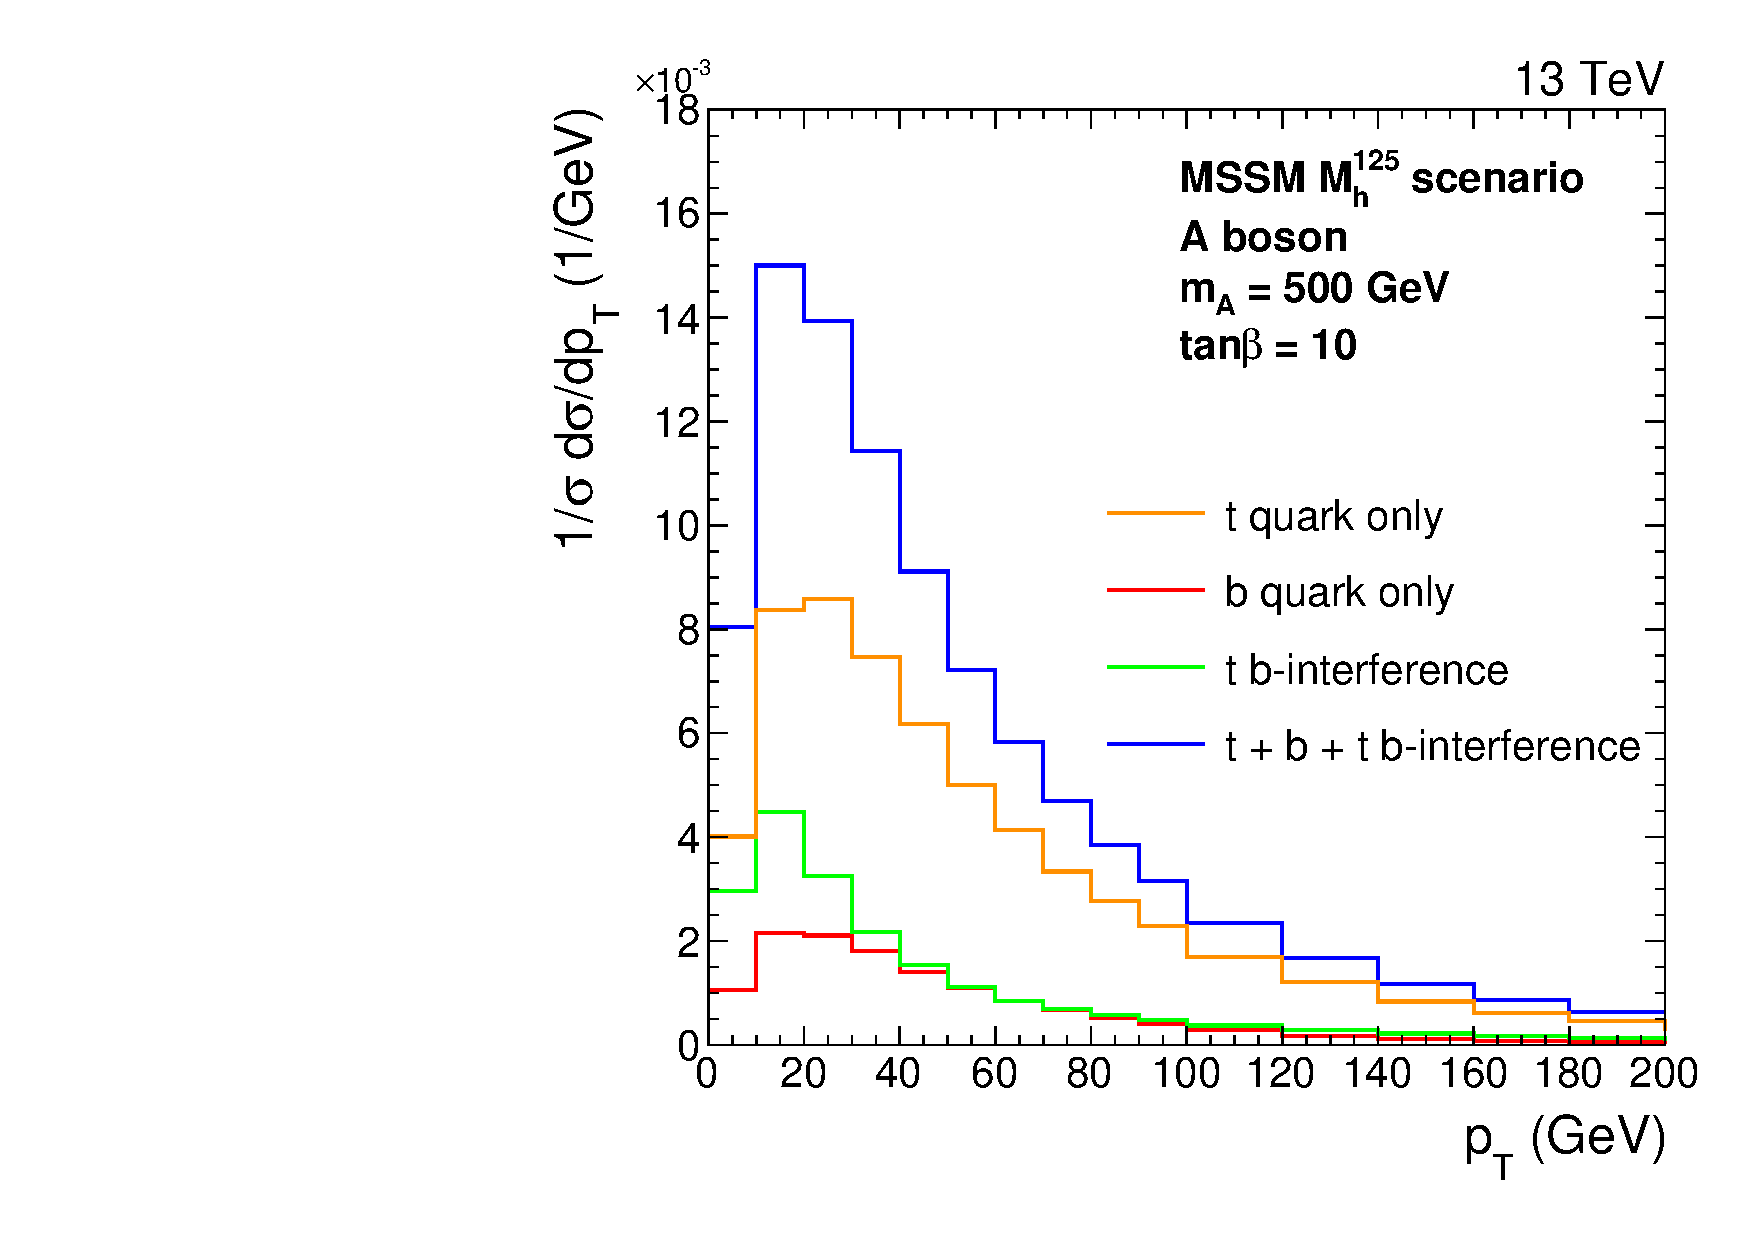
\includegraphics[width=0.5\textwidth]{Figures/pT_reweighting_plot_A10.pdf}}
    \subfloat[]{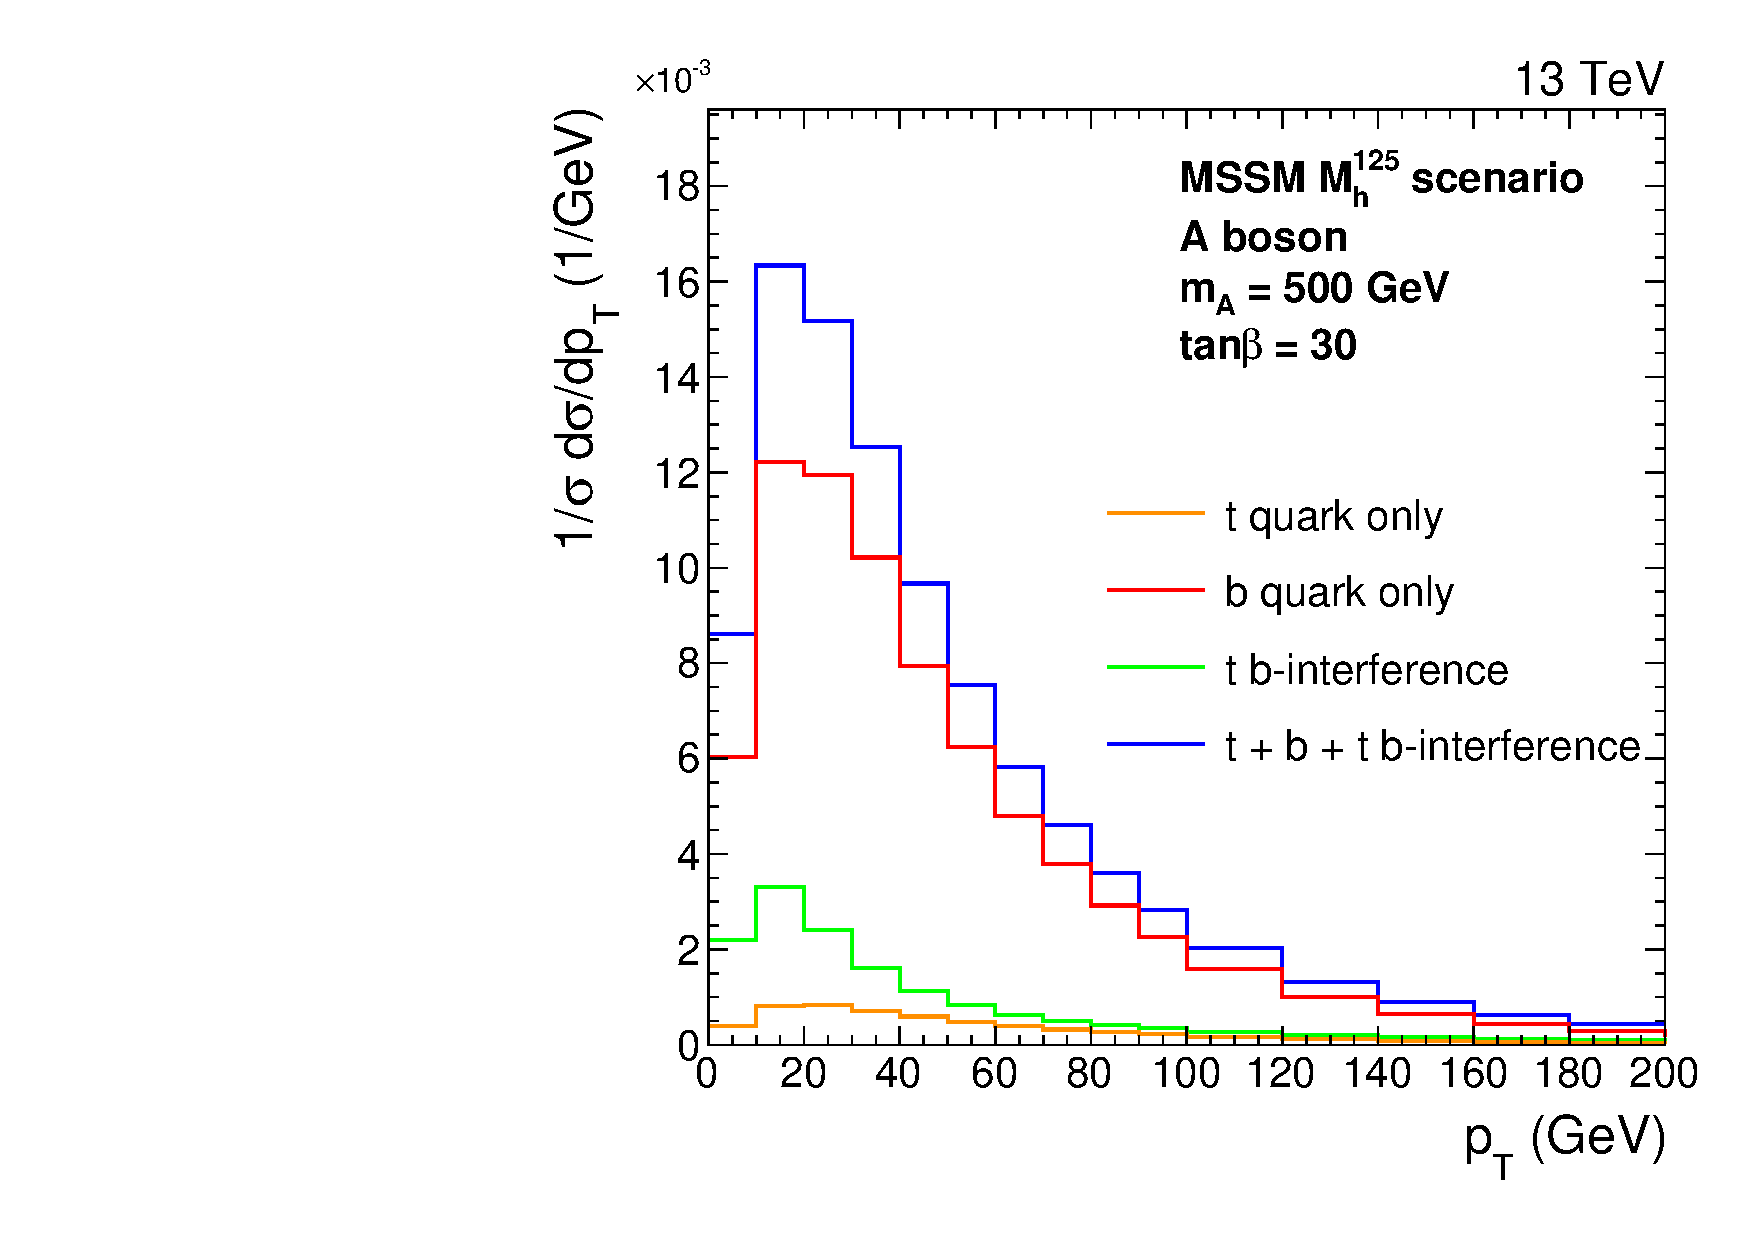
\includegraphics[width=0.5\textwidth]{Figures/pT_reweighting_plot_A30.pdf}} \\
    \subfloat[]{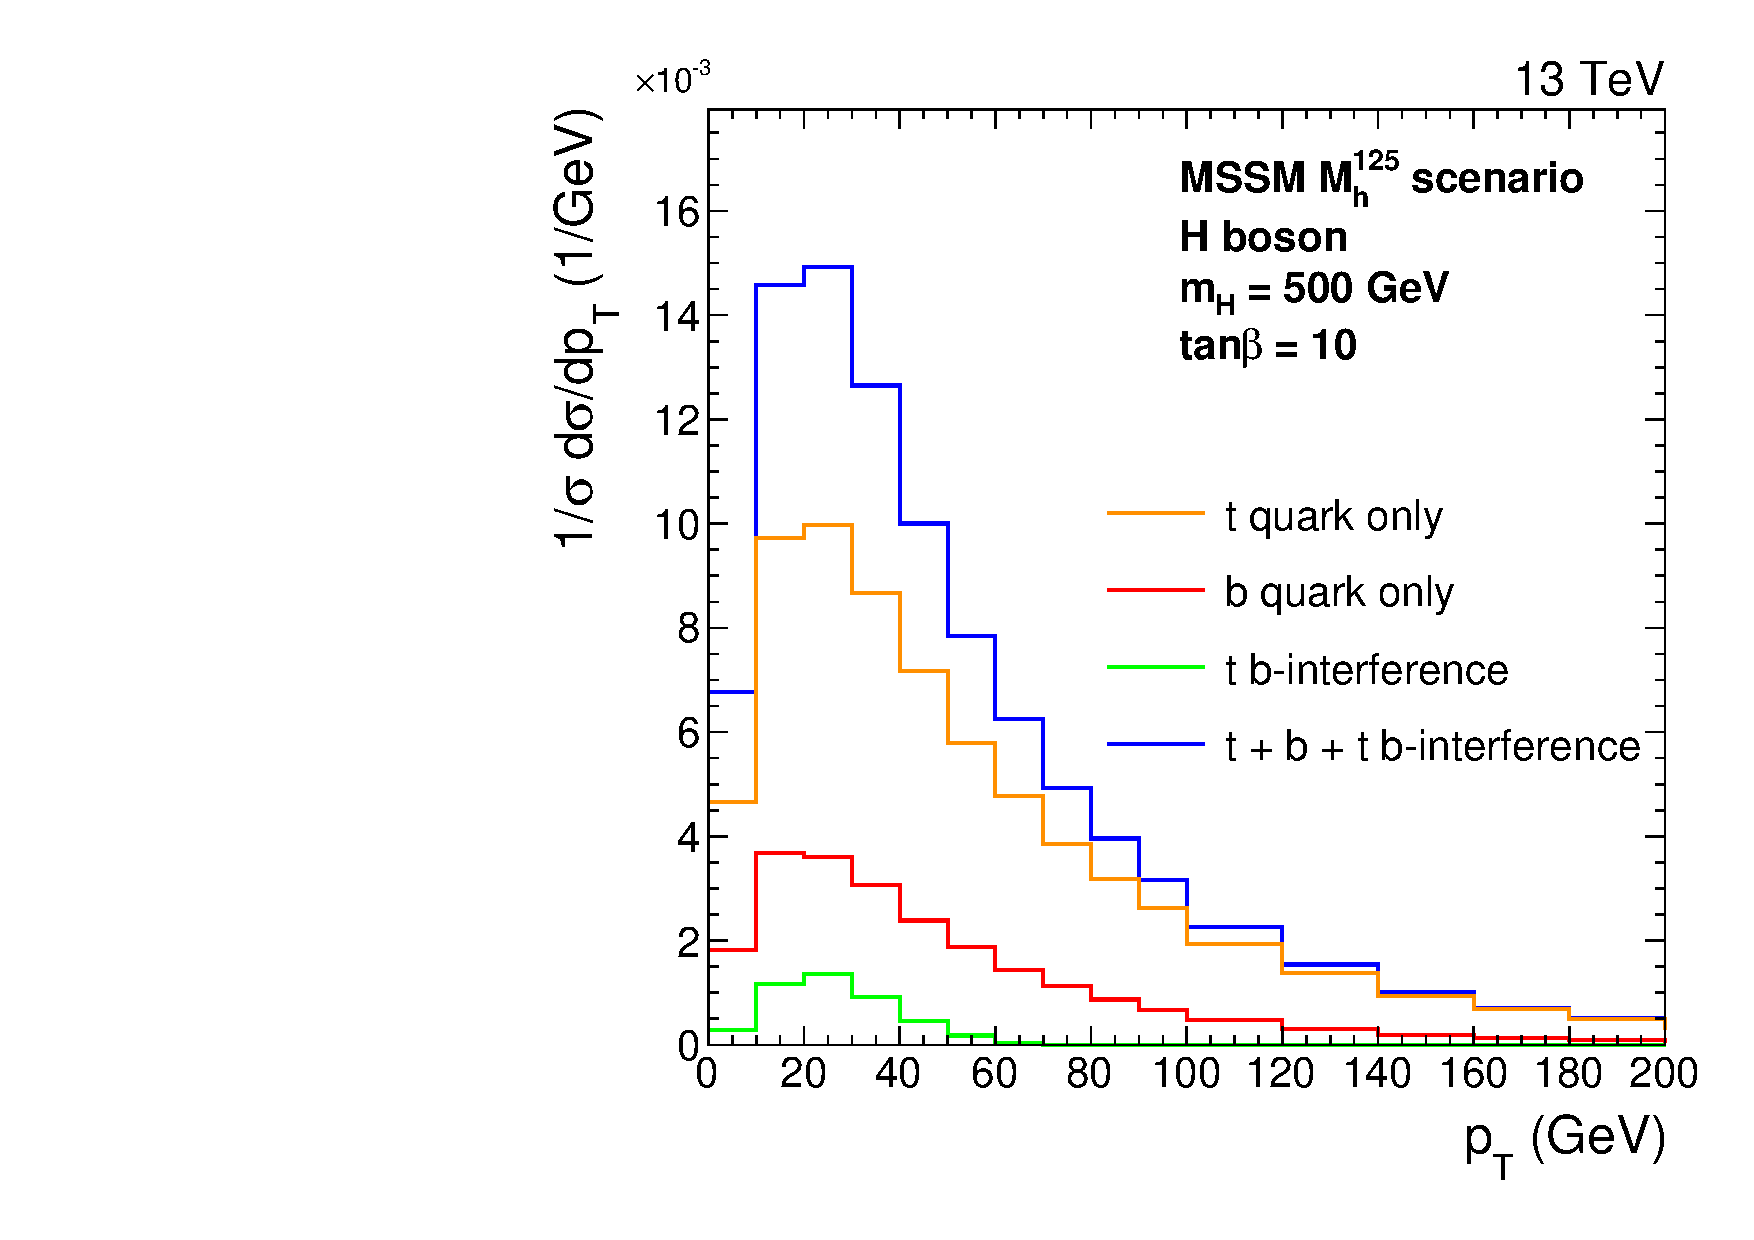
\includegraphics[width=0.5\textwidth]{Figures/pT_reweighting_plot_H10.pdf}}
    \subfloat[]{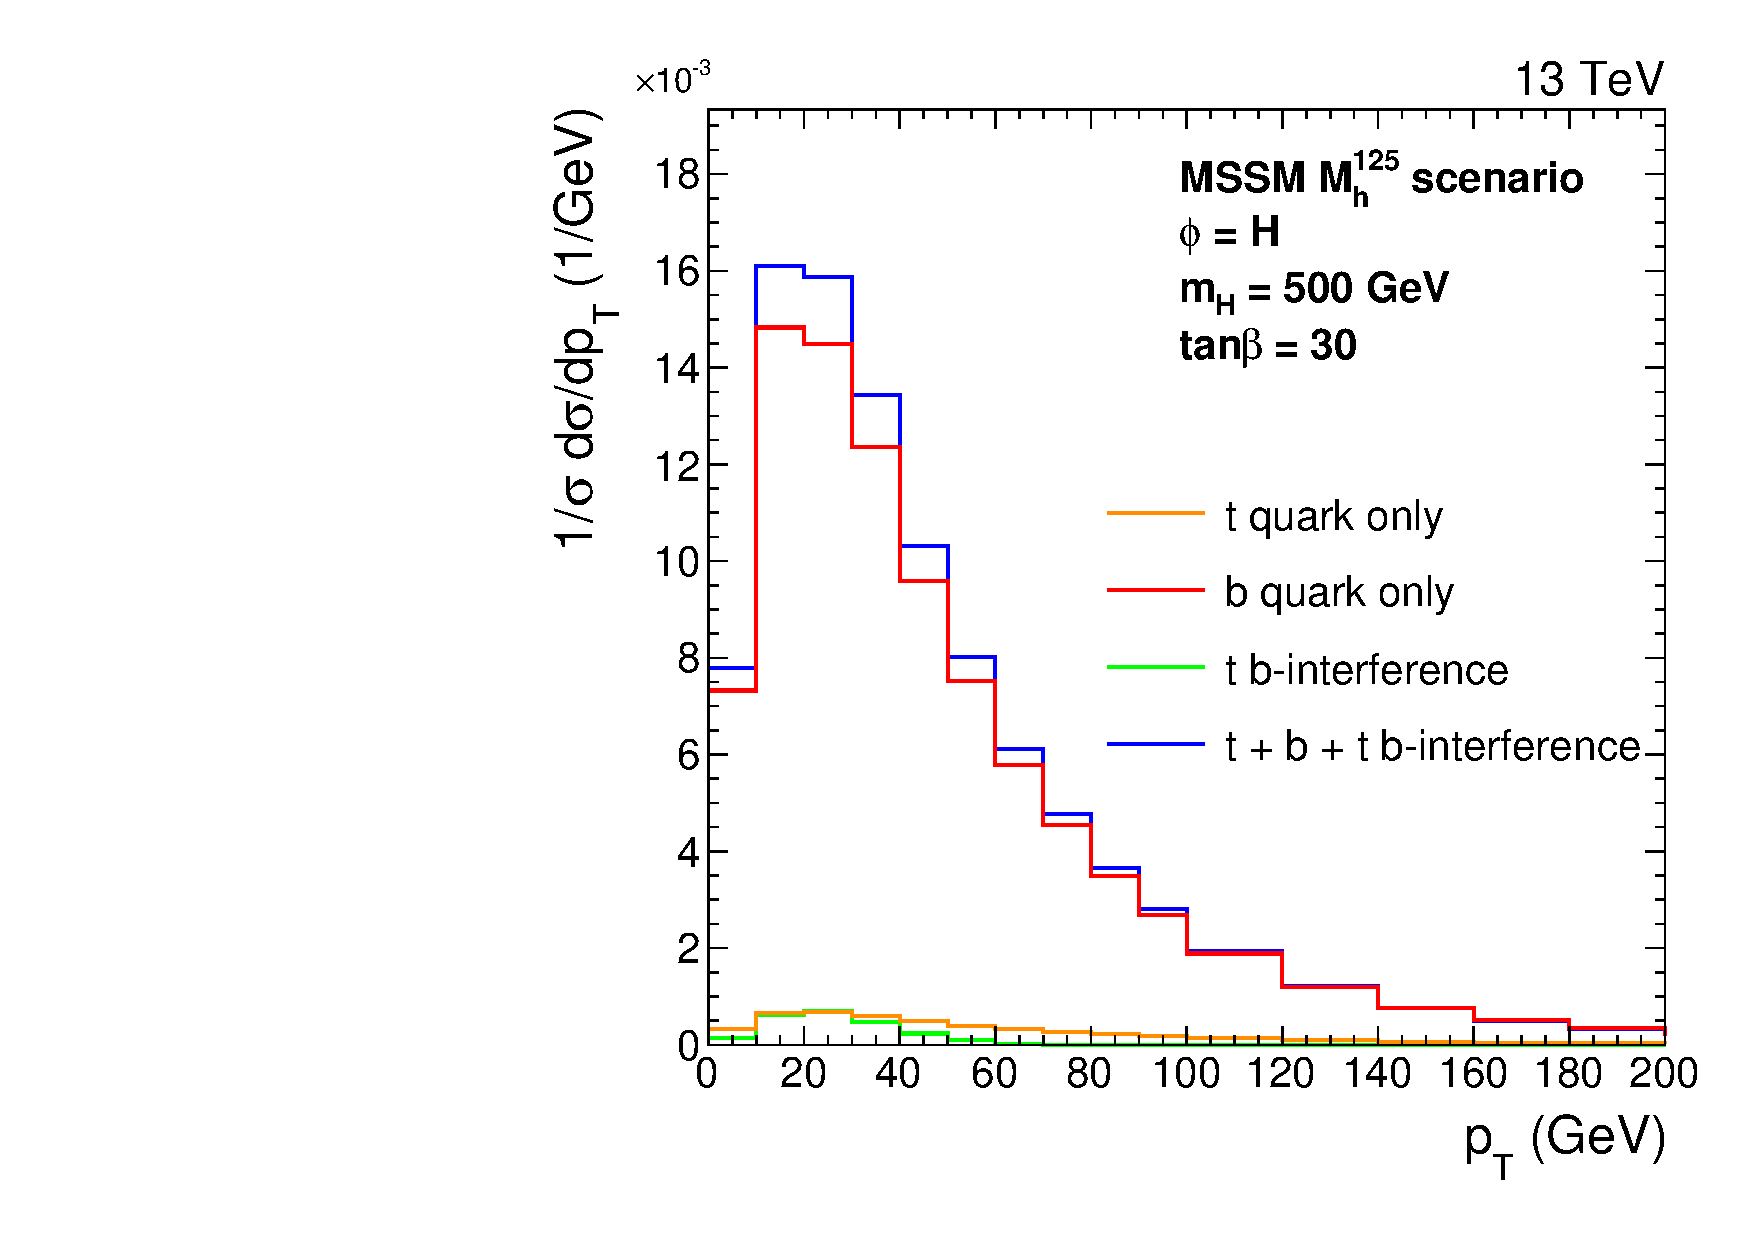
\includegraphics[width=0.5\textwidth]{Figures/pT_reweighting_plot_H30.pdf}} \\
\caption{$p_{T}$ density distributions of the A (top) and H (bottom) boson, with contributions to the gluon fusion loop displayed individually and summed. These are shown for $\tan\beta$ values of 10 (left) and 30 (right) where $m_{A} = 500$ GeV in the MSSM $M_{h}^{125}$ scenario.}
\label{fig:mssm_sig}
\end{figure}

Production in association with bottom quarks is simulated at NLO precision using the corresponding POWHEG 2.0 implementation in the four-flavour scheme.
All additional Higgs boson signal generation is performed using the parton distribution function (PDF) NNPDF3.1.
Tau lepton decay, parton showering and hadronisation are all modelled with the PYTHIA event generator where the PU profile is matched to data.
All events generated are passed through a GEANT4-based simulation of the CMS detector and reconstructed in the same way as data. \\

The model dependent search for the MSSM also looks to find differences from the observed SM Higgs boson and the predicted MSSM SM-like Higgs boson.
In each MSSM benchmark scenario, an uncertainty of $\pm 3$ GeV is given on the prediction for the SM Higgs boson mass.
This uncertainty is to reflect the contribution from any unknown higher-order corrections.
The value of the mass is allowed to vary within this window, however the Yukawa couplings are rescaled the observed mass.

\subsection{Vector Leptoquarks}
\label{sec:vlq}

The best fit in the vector leptoquark phase space to the B anomalies yielded large bottom quark and tau lepton couplings to the $U_1$ particle.
The possible production modes of a $\tau^+\tau^-$ final state are shown in Figure~\ref{fig:leptoquark_feynman}.


\begin{figure}[H]
\centering
\begin{subfigure}[b]{0.3\textwidth}
\begin{tikzpicture}[scale=2]
  \begin{feynman}
    \vertex [label=left:$\bar{q}$] (a1) at (0,0);
    \vertex [label=left:$q$] (a2) at (0,1);
    \vertex (b1) at (1,0);
    \vertex (b2) at (1,1);
    \vertex [label=right:$U_{1}$] (b3) at (1,0.5);
    \vertex [label=right:$\tau^-$] (c1) at (2,0);
    \vertex [label=right:$\tau^+$] (c2) at (2,1);

    \diagram* {
      (b1) -- [fermion] (a1),
      (a2) -- [fermion] (b2),
      (b2) -- [boson] (b1),
      (c1) -- [fermion] (b1),
      (b2) -- [fermion] (c2),
    };
  \end{feynman}
\end{tikzpicture}
\caption{}
\end{subfigure} \\

\begin{subfigure}[b]{0.3\textwidth}
\begin{tikzpicture}[scale=2]
  \begin{feynman}
    \vertex [label=left:$g$] (a1) at (0,0);
    \vertex [label=left:$g$] (a2) at (0,1);
    \vertex (b1) at (0.7,0.5);
    \vertex (b2) at (1.2,0.5);
    \vertex (c1) at (1.7,0.1);
    \vertex (c2) at (1.7,0.9);
    \vertex [label=$U_{1}$] (c1t) at (1.4,-0.05);
    \vertex [label=$U_{1}$] (c2t) at (1.4,0.72);
    \vertex [label=right:$\tau^+$] (d1) at (2.2,1.2);
    \vertex [label=right:$q$] (d2) at (2.2,0.6);
    \vertex [label=right:$\tau^-$] (d3) at (2.2,0.4);
    \vertex [label=right:$\bar{q}$] (d4) at (2.2,-0.2);
    
    \diagram* {
      (a1) -- [gluon] (b1),
      (a2) -- [gluon] (b1),
      (b1) -- [gluon] (b2),
      (b2) -- [scalar] (c1),
      (b2) -- [scalar] (c2),
      (d1) -- [fermion] (c2),
      (c2) -- [fermion] (d2),
      (c1) -- [fermion] (d3),
      (d4) -- [fermion] (c1),
    };
  \end{feynman}
\end{tikzpicture}
\caption{}
\end{subfigure}
\hspace{2cm}
\begin{subfigure}[b]{0.3\textwidth}
\begin{tikzpicture}[scale=2]
  \begin{feynman}
    \vertex [label=left:$g$] (a1) at (0,0);
    \vertex [label=left:$q$] (a2) at (0,1);
    \vertex (b1) at (0.7,0.5);
    \vertex [label=below:$q$] (bt) at (0.95,0.45);
    \vertex (b2) at (1.2,0.5);
    \vertex [label=right:$\tau^-$] (c1) at (2,0);
    \vertex (c2) at (1.7,0.9);
    \vertex [label=$U_{1}$] (c2t) at (1.4,0.72);
    \vertex [label=right:$\tau^+$] (d1) at (2.2,1.2);
    \vertex [label=right:$q$] (d2) at (2.2,0.6);

   
    \diagram* {
      (a1) -- [gluon] (b1),
      (a2) -- [fermion] (b1),
      (b1) -- [fermion] (b2),
      (b2) -- [fermion] (c1),
      (b2) -- [scalar] (c2),
      (d1) -- [fermion] (c2),
      (c2) -- [fermion] (d2),
    };
  \end{feynman}
\end{tikzpicture}
\caption{}
\end{subfigure}

\caption{Feynman diagrams showing the contribution from $U_1$ vector leptoquarks to the final state with a pair of oppositely charged tau leptons. Diagram (a) shows t-channel, (b) pair and (c) single production of a vector leptoquark.}
\label{fig:leptoquark_feynman}
\end{figure}

Pair and single production of a vector leptoquark is dependent on its strong coupling, which is highly model dependent.
For large mass, $m_U$, the probability of producing an on-shell $U_1$ singlet or pair is heavily suppressed due to the momentum of the initial partons.
These production processes are not discussed further in this search.
Further studies have been used to search for single and pair production at the CMS experiment and no statistically significance derivation was observed. \\

The t-channel process contain two vertices with a $U_1$ vector leptoquark, a quark and a tau lepton, and hence the cross section will scale with $g_{U}^4$.
From the best fit to B anomalies this vertex will be dominated by the b quark and hence the initial state will be mostly from $b\bar{b}$, with sub-dominant contributions from $b\bar{s}$, $s\bar{b}$ and $s\bar{s}$.
Although there are no additional b quarks in the final state in the LO process, initial state radiation can lead to additional b quarks in the final state.
In this search the two scenarios discussed in Section~\ref{sec:introduction} are considered.
The only non negligible parameter for $\tau^{+}\tau^{-}$ final states from the fit in the $m_{U}$-$g_{U}$ phase space is the $\beta_{L}^{s\tau}$ parameter.
This is set to the best fit value. \\

The signal process of the $U_1$ t-channel exchange is simulated in the five-flavour scheme (5FS) at LO precision using the \MGvATNLO event generator, v2.6.5.
Events are generated with one or fewer outgoing partons from the matrix element and the MLM prescription is then used for matching, with a scale set to 40 GeV.
Negligible dependence of the $U_1$ decay width ($\Lambda$) is observed, for simulation this is chosen to approximately match the value predicted by the B anomaly fit.
Samples with a mass between 1 and 5 TeV at $g_U = 1$ are generated. \\

The interference between the $U_1$ signal and $Z/\gamma^* \rightarrow \tau\tau$ production was checked.
A large destructive affect is observed, with the magnitude dependent on $g_{U}$.
To account for this, separate samples are produced for this interference, generated in the same way as the t-channel exchange.
The interference samples are then split into two with a di-tau mass split in order to have a sufficient number of events in the high di-tau mass regions.
The cross section of these interference samples scale with $g_{U}^2$. 
Examples of the generator level di-tau mass distributions are shown in Figure~\ref{fig:vlq_signal}. \\

\begin{figure}[!hbtp]
\centering
    \subfloat[]{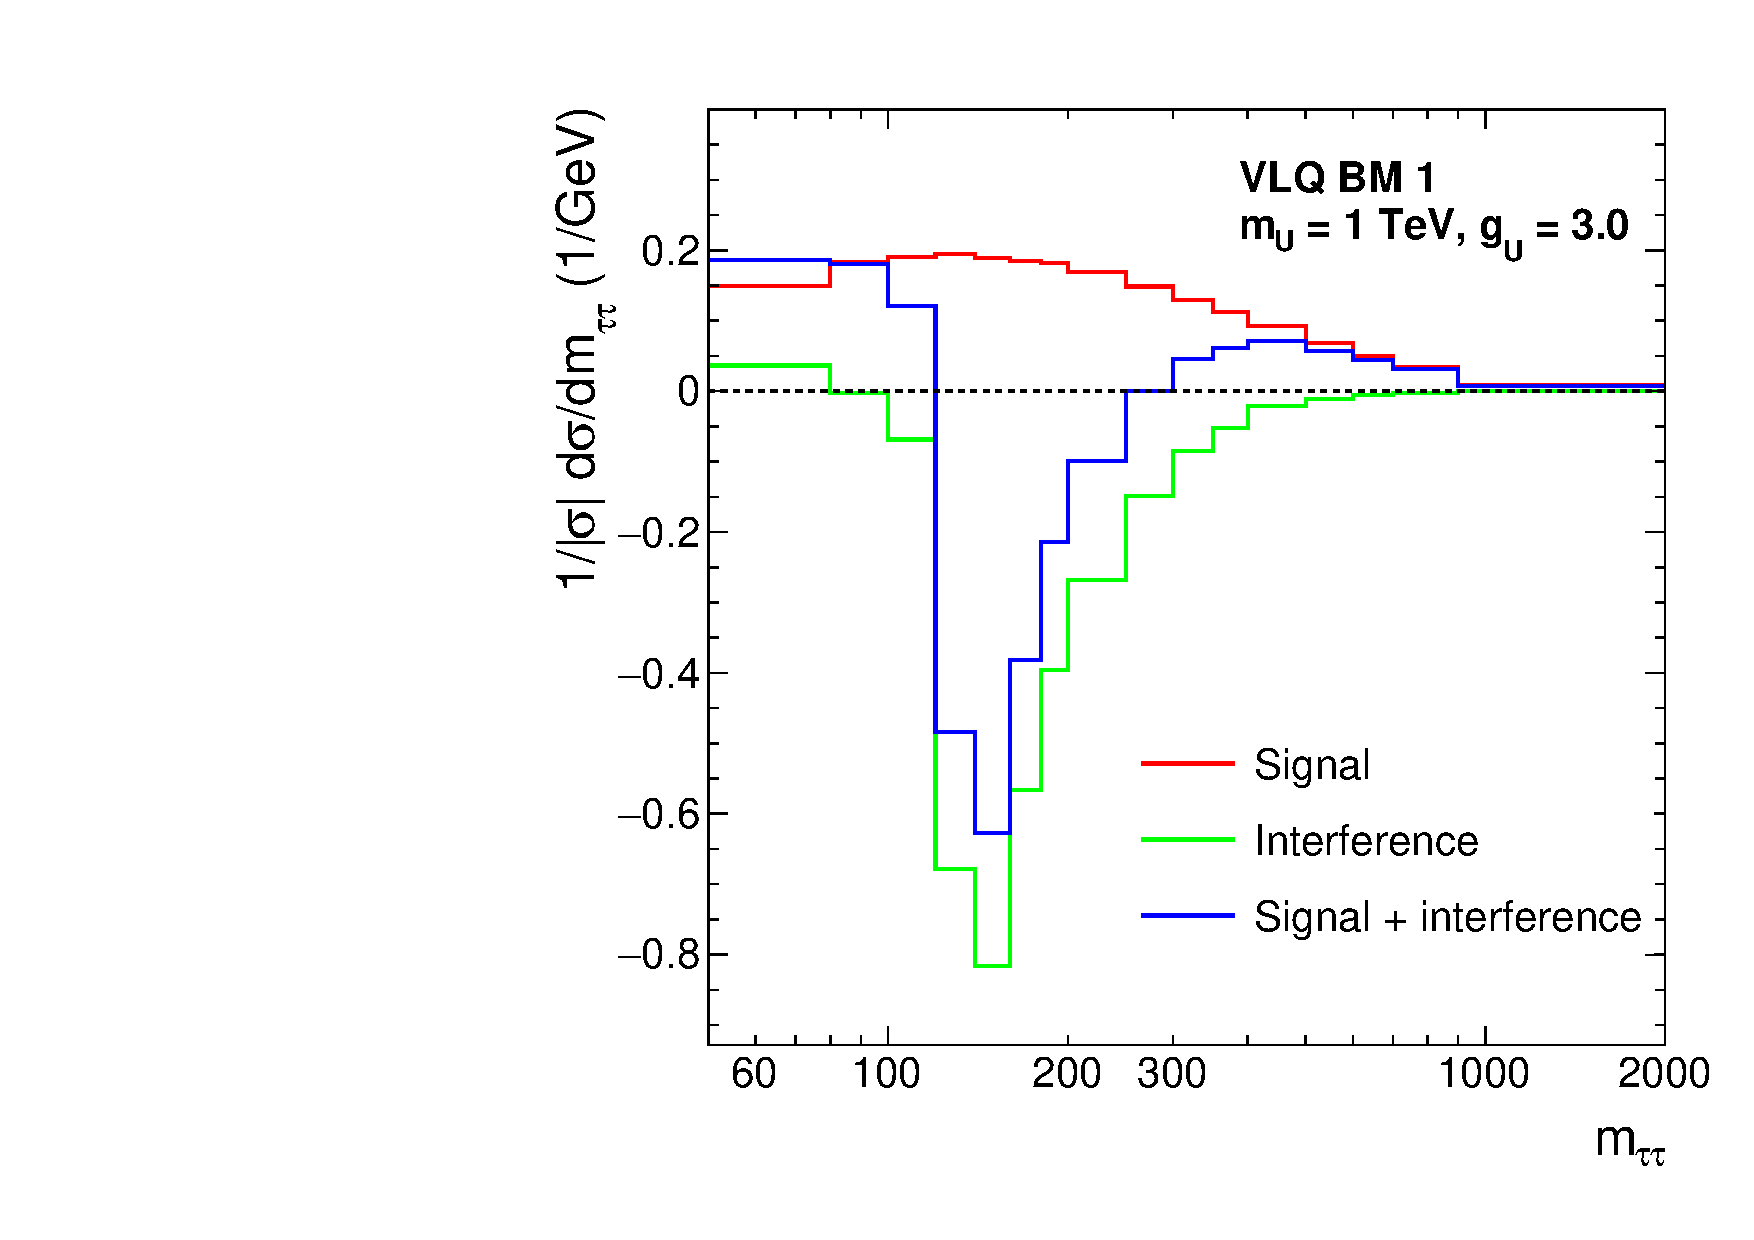
\includegraphics[width=0.5\textwidth]{Figures/vlq_signal_plot_gU3.pdf}}
    \subfloat[]{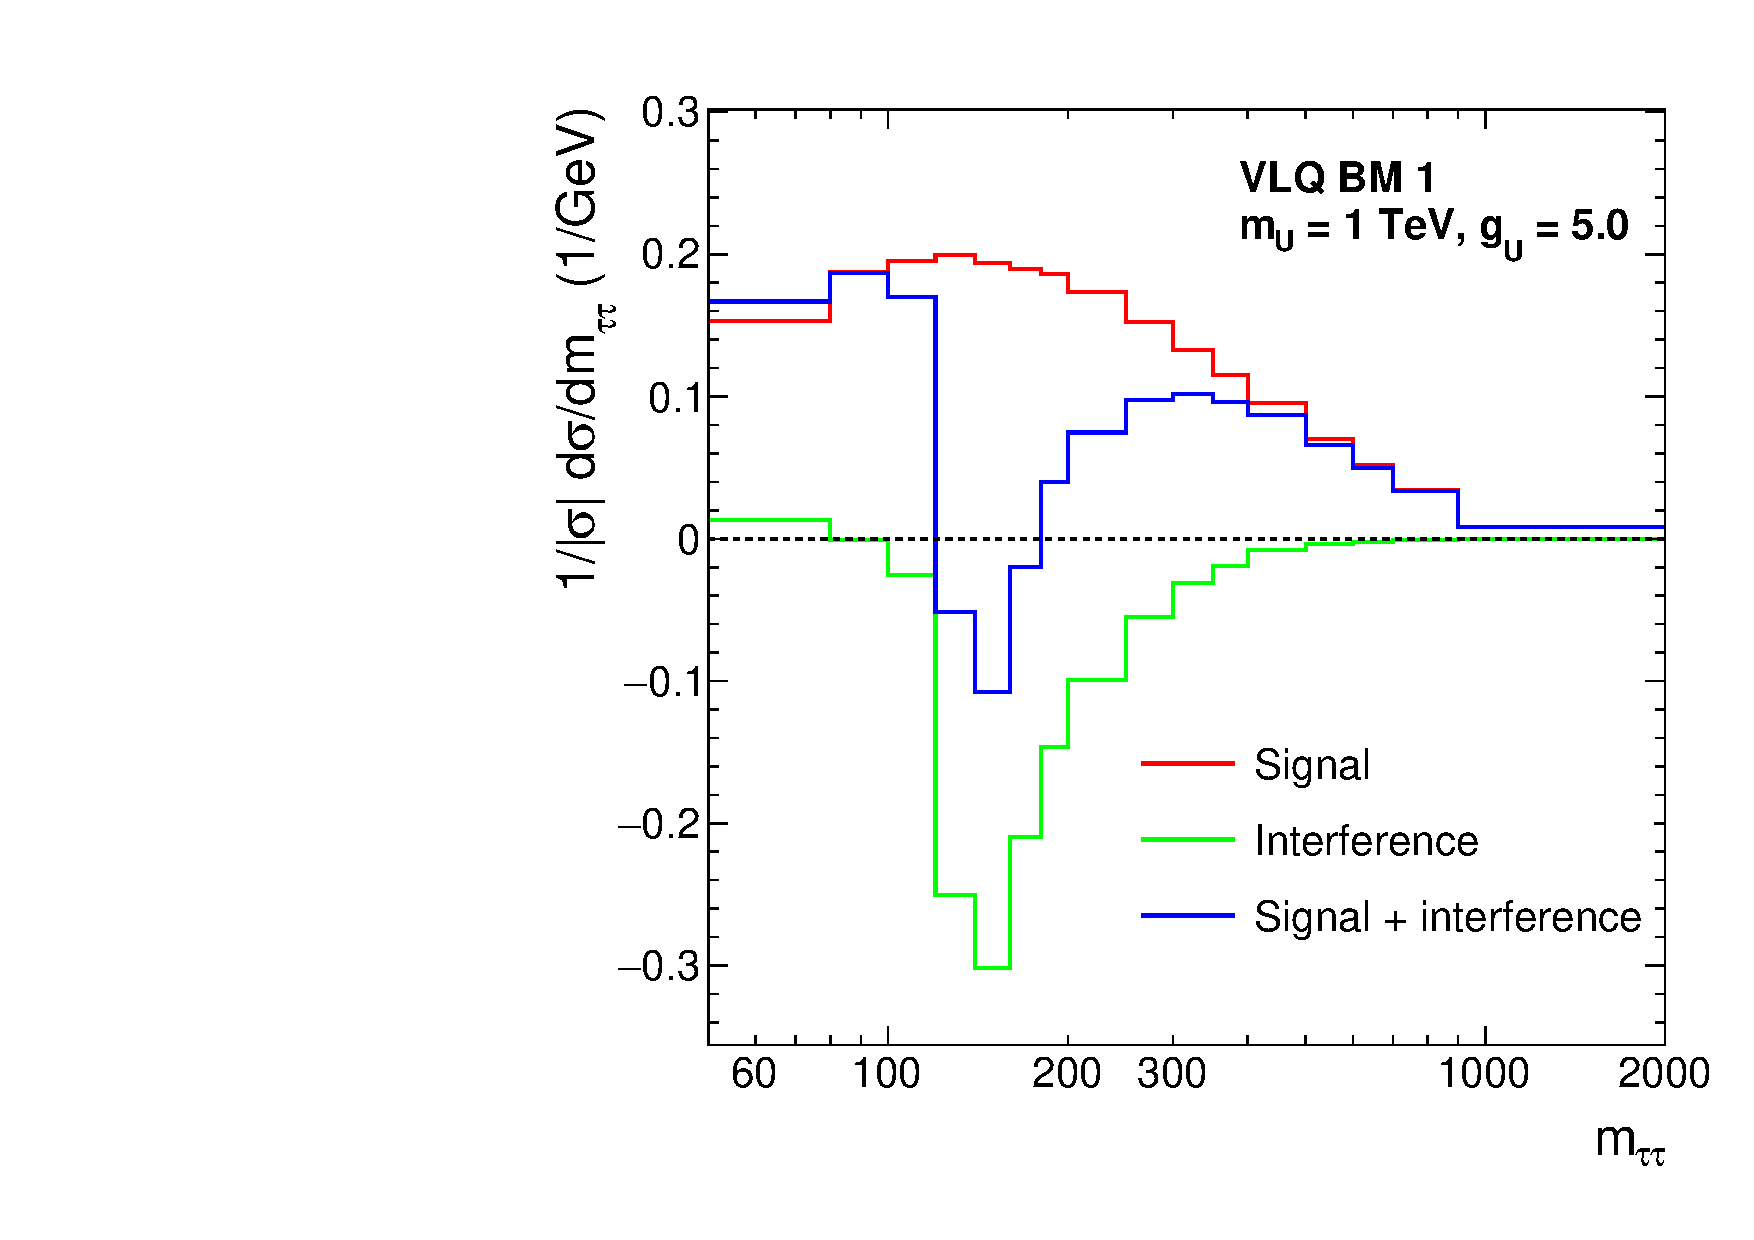
\includegraphics[width=0.5\textwidth]{Figures/vlq_signal_plot_gU5.pdf}}
\caption{The generator level $m_{\tau\tau}$ density distributions of the t-channel vector leptoquark signal and the interference with Drell-Yan. This is shown in the VLQ BM 1 scenario for a leptoquark of mass 1 TeV for coupling strengths of $g_{U}=3$ (a) and $g_{U}=5$ (b).}
\label{fig:vlq_signal}
\end{figure}

The t-channel signal produces a broad distribution in $m_{\tau\tau}$ due to its non-resonant nature.
The interference is mostly a destructive effect (except for at small $m_{\tau\tau}$), with the yield becoming less negative at higher $m_{\tau\tau}$.
The interference peaks negatively between 100 and 200 GeV and in this region the combined yield can be negative.
Due to the difference in scaling of the two effects, at small $g_{U}$ the interference is more dominant than the signal and hence the yield of the combined result is reduced.

\section{Event Selection}

The possible decays of two tau leptons and their branching fractions, where the tau decay is grouped into three categories e, $\mu$ and $\tau_h$ as defined in Section~\ref{sec:object_reconstruction}, are shown in Table~\ref{tab:ditau_br}. 
For this search the four largest branching fraction channels used: $\tauhtauh$, $\etauh$, $\mutauh$ and $e\mu$.
This accounts for approximately 94\% of di-tau events.
The two same lepton channels are neglected due to small branching ratio and the dominating $Z\rightarrow ee$ and $Z\rightarrow \mu\mu$ backgrounds. \\

\begin{table}[!hbtp]
    \centering
    \begin{tabular}{|c|c|}
         \hline
         Channel & Branching Fraction  \\
         \hline
         \hline
         $\tauhtauh$ & 42.0\% \\
         $\etauh$ & 23.1\% \\
         $\mutauh$ & 22.6\% \\
         $\emu$ & 6.2\% \\
         $e e$ & 3.2\% \\
         $\mu \mu$ & 3.0\% \\
         \hline
    \end{tabular}
    \caption{Branching fractions of the decays of two tau leptons.}
    \label{tab:ditau_br}
\end{table}

\subsection{Trigger Requirements}

In the four final state pairs a number of different online trigger requirements are needed.
In the $\tauhtauh$ channel, two possible triggers are available: the double-$\tauh$ and single-$\tauh$ triggers.
The single-$\tauh$ trigger has a high $\pT$ threshold at 120 (180) GeV for events recorded in 2016 (2017-2018), whilst the double-$\tauh$ has a $\pT$ threshold at 40 GeV.
Therefore, the double-$\tauh$ trigger is used individually where the $\tauh$ has $\pT$ is below the single-$\tauh$ threshold and the union of single-$\tauh$ and double-$\tauh$ triggered events are taken above the threshold. \\

In the $\etauh$ and $\mutauh$ channels, there are three possible triggers available: the single-e/$\mu$, single-$\tauh$ and the e/$\mu$-$\tauh$ cross-trigger.
The cross-trigger is used for events where the light lepton has $\pT$ between the thresholds for the cross-trigger and single-$e/\mu$ shown in Table~\ref{tab:trig_thresholds}.
The light lepton used in the cross-trigger is required to be in the central barrel of the detector within $|\eta| < 2.1$.
Above these light lepton $\pT$ thresholds the single-$e/\mu$ trigger is used, where here it is required that the $\tauh$ has $\pT >$ 30 GeV.
At $\tauh$ $\pT$ above the single-$\tauh$ thresholds, the single-$\tauh$ trigger is used in combination with the single-$e/\mu$ trigger. \\

\begin{table}[hbtp]
  \centering
  \begin{tabular}{|c||c|c|c|c|}
    \hline
    Year/ Trigger   & $\etauh$ cross-trigger & single-$e$ & $\mutauh$ cross-trigger & single-$\mu$ \\
    \hline
    \hline
    2016 & 23                    & 26         & 20                     & 23           \\
    2017 & 25                    & 28         & 20                     & 25           \\
    2018 & 25                    & 33         & 21                     & 25           \\
    \hline        
  \end{tabular}
  \caption{Lower trigger light lepton thesholds $\pT$ in GeV for the $\etauh$ and $\mutauh$ channels.}
  \label{tab:trig_thresholds}  
\end{table}

In the $\emu$ channel, there are three possible triggers available: the single-$e$, single-$\mu$ and the e-$\mu$ cross-trigger.
However, only the cross-trigger is used in this analysis, due to the larger efficiencies of correctly selecting light leptons.
The e and $\mu$ are required to have $\pT >$ 15 GeV and $|\eta| < 2.4$.

\subsection{Offline Requirements}

All offline selections stated are in addition the object selection discussed in Section~\ref{sec:object_reconstruction}.
In this analysis, hadronic tau candidates are required to pass the \texttt{Medium} $D_{\text{jet}}^{\text{WP}}$.
$D_{e}^{\text{WP}}$ and $D_{\mu}^{\text{WP}}$ are dependent on the channel.
The \texttt{VVLoose}, \texttt{Tight}, \texttt{VVLoose} $D_{e}^{\text{WP}}$ and the \texttt{VLoose}, \texttt{VLoose} and \texttt{Tight} $D_{\mu}^{\text{WP}}$ are used in the $\tauhtauh$, $\etauh$ and $\mutauh$ channels respectively.
The tighter working point for the same light lepton discrimination as tagged in the event is used to remove light leptons faking hadronic taus from the $Z \rightarrow ll$ process.
The light lepton isolation requirement is $\Irel^{e/\mu} < 0.15$ except for in the $\emu$ channel where the muon is required to have $\Irel^{\mu} < 0.2$. \\

The selected $\tau$ lepton decay candidates are required to have opposite charge and to be separated by more than $\Delta R$ > 0.5 in all channels except $\emu$ where $\Delta R$ > 0.3.
In events where the numbers of an object in the event is greater than the required number of objects in the $\tau\tau$ decay channel, the objects are sorted by the maximum $D_{\text{jet}}^{\text{score}}$ if $\tau_h$ or minimum $\Irel$ if a light lepton and the leading objects are chosen.
In order to maintain orthogonality between channels, events with additional light leptons passing looser selections than the nominal requirements, are rejected from the selection.
The looser selections help to suppress the $Z \rightarrow ll$ background process further. \\

In the $\etauh$ and $\mutauh$ channels, a cut is placed at 70 GeV on the transverse mass between the light lepton $\pTvec$ and the missing $\pTvec$, where the transverse momentum is defined as,
\begin{equation}
m_{\text{T}}(\pTvec^{\hspace{2pt}i},\pTvec^{\hspace{2pt}j}) = \sqrt{2\pT^{i}\pT^{j}(1-\cos\Delta\phi)},
\end{equation}
where $\Delta\phi$ to the azimuthal angle between $\pTvec^{\hspace{2pt}i}$ and $\pTvec^{\hspace{2pt}j}$.
The variable is used to remove W + jets background events, where a jet fakes a hadronic tau and the MET and light lepton from the W decay are aligned and hence the event has a large $m_{T}(\pTvec^{\hspace{2pt}e/\mu},\pTvec^{\hspace{2pt}\text{MET}})$.

In the $\emu$ channel an additional cut is placed on a variable named $D_{\zeta}$, which is defined as,
\begin{equation}
D_\zeta = p_\zeta^\text{miss} - 0.85 p_\zeta^\text{vis};\qquad
p_\zeta^\text{miss} = \pTvec^{\hspace{2pt}\text{miss}} \cdot \hat{\zeta};\qquad
p_\zeta^\text{vis} = (\pTvec^{\hspace{2pt}e} + \pTvec^{\hspace{2pt}\mu}) \cdot \hat{\zeta}
\label{eq:Dzeta_def}
\end{equation}
where $\pTvec^{\hspace{2pt}e/\mu}$ corresponds to the transverse momentum vector of the electron or muon and $\hat{\zeta}$ to the bisectional direction between the electron and the muon in the transverse plane~\cite{CDFPzeta}.
A diagram of the inputs is shown Figure~\ref{fig:dzeta_diagram}.
\begin{figure}[!hbtp]
\centering
    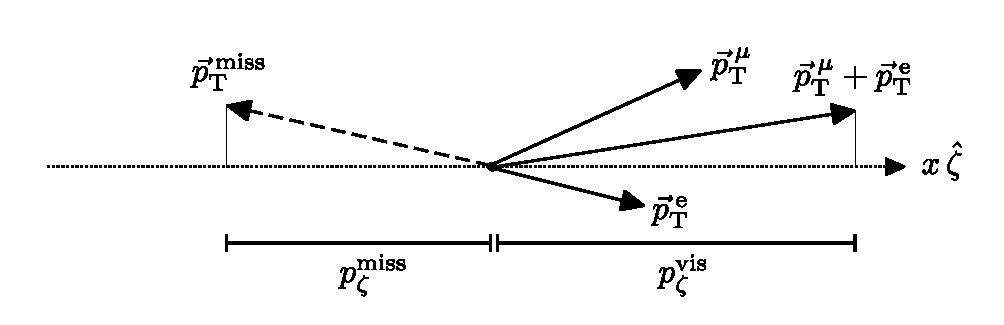
\includegraphics[width=1.0\textwidth]{Figures/dzeta_diagram.pdf}
\caption{Diagram of inputs to the $D_\zeta$ variable.}
\label{fig:dzeta_diagram}
\end{figure}
The linear combination is optimised for genuine di-tau events to peak around $D_{\zeta} = 0$ GeV. 
It is motivated by the expectation that in di-tau decays from a resonance, the visible and missing (from tau neutrinos) momentums are roughly aligned and of similar magnitudes.
In W + jets and $\ttbar$ events the directions of the visible and missing products are expected to be more randomly distributed and lead to a non-peaking $D_{\zeta}$.
Therefore only events with $D_\zeta >$ -35 GeV are considered for signal events.
No b tagged events with this cut are vetoed and b tagged events with this cut are used for a $\ttbar$ control region and discussed further in Section~\ref{sec:background_modelling}.

\section{Signal Extraction}

The optimisation of the signal extraction depends on which of the three scenarios, set out at beginning of this section, is searched for.
The components of the optimisation are named the high mass, low mass and SM Higgs optimisation procedures.
For the model independent search (i) the high or low mass optimisation procedures are used depending on whether the mass of the resonance is greater or less than 250 GeV.
The search for the MSSM Higgs sector (ii) uses the high mass or the SM Higgs optimisation procedures depending on whether the reconstructed di-tau mass \cite{} is greater or less than 250 GeV.
Finally, the search for vector leptoquarks (iii) uses only the high mass optimisation procedure.
The procedures are discussed in detail below. \\

The high mass optimisation procedure follows what was done in Ref. \cite{}.
Firstly each category is split into categories with no b tagged and with one or more b tagged events.
This firstly helps target the additional Higgs boson production modes gluon fusion and b associated production respectively.
Secondly, the initial state radiation of a t-channel vector leptoquark signal dominated by initial states of b quarks, can lead to additional b jets in the final state.
The reduced backgrounds in b tagged events allows for a more sensitive vector leptoquark search in this category. \\

The $\etauh$ and $\mutauh$ channels are further subdivided into catego


The corresponding categories in $\etauh$ and $\mutauh$ channels are defined by
\begin{itemize}
\item \texttt{Tight-$m_{\text{T}}$}: $m_{\text{T}}^{e/\mu} [\GeV] < 40$;
\item \texttt{Loose-$m_{\text{T}}$}: $40 \leq m_{\text{T}}^{e/\mu} [\GeV] < 70$.
\end{itemize}
The bulk of the signal events, particularly for low mass hypotheses, lies in the \texttt{Tight-$m_{\text{T}}$} sub-category.
The \texttt{Loose-$m_{\text{T}}$} category has been added to increase the signal acceptance for mass hypotheses of $m_{A,H} > 700$~\GeV.

In the $\emu$ final state, three sub-categories are defined by
\begin{itemize}
\item \texttt{Low-$D_\zeta$}: $-35 \leq D_\zeta [\GeV] < -10$;
\item \texttt{Medium-$D_\zeta$}: $-10 \leq D_\zeta [\GeV] <  30$;
\item \texttt{High-$D_\zeta$}: $D_\zeta [\GeV] \geq 30$.
\end{itemize}
In this way sub-categories with different signal purities and $\ttbar$ fractions can be exploited during the statistical inference for the signal.
The expected signal, for all masses tested, is mostly located in the \texttt{Medium-$D_\zeta$} sub-category.

\begin{figure}[!hbtp]
\centering
    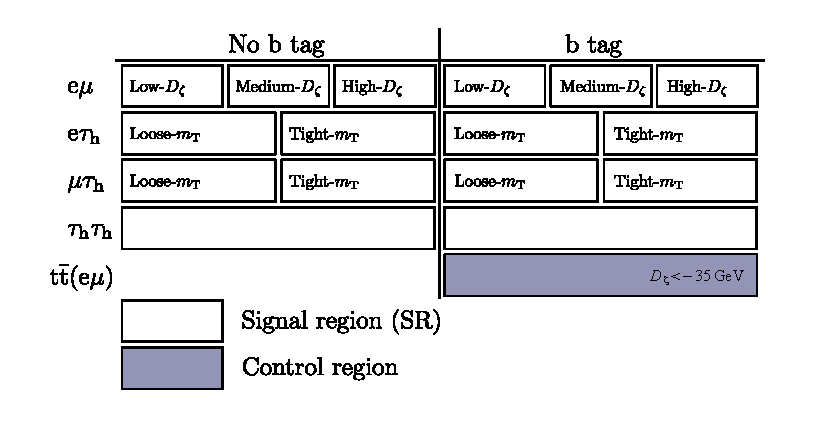
\includegraphics[width=1.0\textwidth]{Figures/high_mass_categories.pdf}
\caption{Overview of the categories used for the extraction of the signal in the high mass optimisation procedure.}
\label{fig:high_mass_categories}
\end{figure}

\begin{equation}
m_{T}^\text{tot} = \sqrt{m_{T}(\pTvec^{\hspace{2pt}\tau_1},\pTvec^{\hspace{2pt}\text{miss}})^2 +  m_{T}(\pTvec^{\hspace{2pt}\tau_2},\pTvec^{\hspace{2pt}\text{miss}})^2 + m_{T}(\pTvec^{\hspace{2pt}\tau_1},\pTvec^{\hspace{2pt}\tau_2})^2}
\end{equation}

\begin{figure}[!hbtp]
\centering
    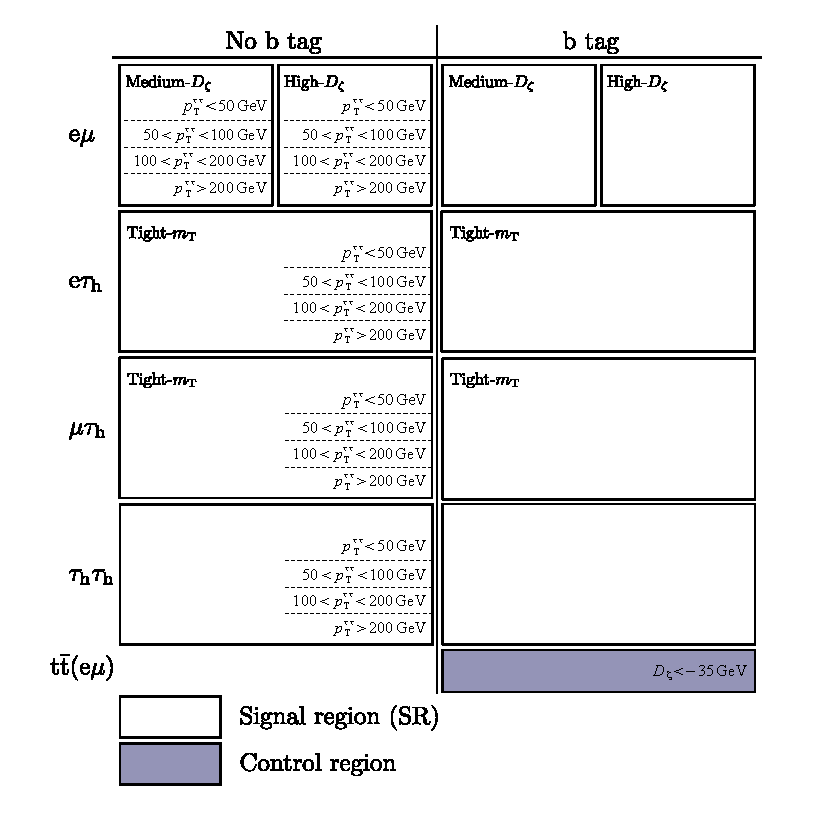
\includegraphics[width=1.0\textwidth]{Figures/low_mass_categories.pdf}
\caption{Overview of the categories used for the extraction of the signal in the low mass optimisation procedure.}
\label{fig:low_mass_categories}
\end{figure}

\section{Background Modelling Overview}
\label{sec:background_modelling}

The analysis considers several backgrounds including Drell-Yan, $\ttbar$, W+jets, QCD, di-boson, single-top, and electroweak W and Z bosons production.
These are split into a five categories:
\begin{enumerate}[i)]
  \item Events containing only genuine tau leptons.
  \item Events with a jet misidentified as a hadronic tau (jet$\rightarrow \tauh$) in the $\etauh$, $\mutauh$ or $\tauhtauh$ channels.
  \item Events with jets faking both light leptons (jet$\rightarrow l$) in the $\emu$ channel.
  \item Events from $\ttbar$ with a prompt light lepton ($e$ or $\mu$ not from a $\tau$ decay) and the other object (if there are not two prompt light lepton) is from a genuine tau leptons.
  \item Other events. This is a small contribution and hence why it is grouped.
  \begin{itemize}
    \item Non $\ttbar$ events with a prompt light lepton ($e$ or $\mu$ not from a $\tau$ decay) and the other object (if there are not two prompt light lepton) is from a genuine tau leptons.
    \item Events with a light lepton faking a hadronic tau and the other object (if there are not two light leptons faking a hadronic tau) are reconstructed as prompt light lepton or from genuine tau leptons. 
    \item Events with a jet faking a light lepton and the other object is from genuine tau leptons in the $\etauh$, $\mutauh$ or $\tauhtauh$ channels.
    \item Events with one jet faking a light lepton and the other object from a prompt light lepton in the $\emu$ channel.
   \end{itemize}
\end{enumerate}

Backgrounds from (i) consists of largely Z/$\gamma^* \rightarrow \tau\tau$ events but there are also smaller contributions from other processes. 
This background is modelled by a data-simulation hybrid method called the embedding method and this is described in detail in Section~\ref{sec:embedding}.
Group (ii) is dominated by QCD, W + jets and $\ttbar$ events with a jet$\rightarrow \tauh$ misidentification.
This is modelled from data by the fake factor method ($\FF$) and is explained in Section~\ref{sec:ff}.
Group (iii) is modelled from data to describe QCD multijet contribution to the background in the $\emu$ channel.
The method to obtain this background is described in Section~\ref{sec:qcd}.
The data driven background estimations for (i), (ii) and (iii) contribute >98\% of all expected background events in the $\tauhtauh$ channel, >90\% in $\etauh$ and $\mutauh$ channels and >50\% in the $\emu$ channel.
The final groups, (iv) and (v), are modelled with MC.
The $\ttbar$ process is separated due to its large contribution to the phase space where a b jet is required. \\

The W + jets and $Z\rightarrow ll$ processes are simulated at leading order (LO) using the \MGvATNLO 2.2.2 (2.4.2) event generator~\cite{Alwall:2011uj,Alwall:2014hca} for the simulation of the data taken in 2016 (2017--2018). 
To increase the number of simulated events in regions of high signal purity, supplementary samples are generated with up to four outgoing partons in the hard interaction. 
For diboson production, \MGvATNLO is used at next-to-LO (NLO) precision. 
In each case, the FxFx~\cite{Frederix:2012ps} (MLM~\cite{Alwall:2007fs})  prescription is used to match the NLO (LO) matrix element calculation with the parton shower model. 
For $\ttbar$~\cite{Alioli:2011as} and (t-channel) single top quark production~\cite{Frederix:2012dh}, samples are generated at NLO precision using \POWHEG 2.0~\cite{Nason:2004rx,Frixione:2007vw,Alioli:2010xd,Jezo2015aia}. 
The \POWHEG version 1.0 at NLO precision is used for single top quark production in association with a W boson (tw channel)~\cite{Re:2010bp}. 

When compared with data, W + jets, $Z\rightarrow ll$, $\ttbar$, and single top quark events in the tW channel are normalised to their cross sections at next-to-NLO (NNLO) precision~\cite{Melnikov:2006kv,Czakon:2011xx,Kidonakis:2013zqa}. 
Single top quark (t-channel) and diboson events are normalized to their cross sections at NLO precision or higher~\cite{Kidonakis:2013zqa,Campbell:2011bn,Gehrmann:2014fva}.



\section{QCD Estimation in the $\emu$ Channel}
\label{sec:qcd}

\section{Embedding Method}
\label{sec:embedding}

\begin{figure}[!hbtp]
\centering
    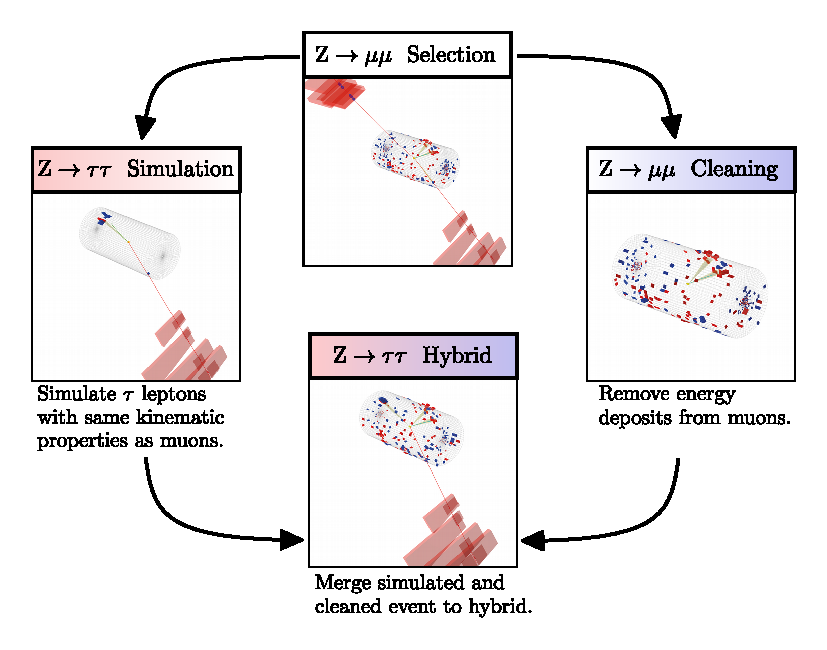
\includegraphics[width=0.8\textwidth]{Figures/Embedding_Diagram.pdf}
\caption{Schematic of the embedding method to model genuine di-tau backgrounds from di-muon events in data.}
\label{fig:embedding}
\end{figure}

Validation plots of it working

\section{Fake Factor Method}
\label{sec:ff}

Backgrounds in which a jet fakes a $\tauh$ can be difficult to model using MC due to the poor description of the $\text{jet}\rightarrow\tauh$ fake rate in simulation. 
In addition, the small probability of a jet being misidentified as a $\tauh$ necessitates the production of high statistics MC samples at a significant computational expense.
These shortcomings motivate the use of data-driven estimates for these processes. 
One such procedure is the fake factor ($\FF$) method. \\

The $\FF$ method utilises regions in the data to model the $\text{jet}\rightarrow\tauh$ background. 
Firstly, the determination regions (DR), which are $\text{jet}\rightarrow\tauh$ enriched control regions orthogonal to the signal region (SR). 
It is used to calculate $\FF$ by taking the ratio of number of jet fake events that pass the nominal hadronic tau ID requirement ($N(\texttt{Nominal})$), to the number of jet fake events that fail the nominal hadronic tau ID but pass a looser alternative hadronic tau ID requirement ($N(\texttt{Alternative}~\&\&~\texttt{!Nominal})$), as shown in Equation~\ref{eqn:ff}.

\begin{equation}
\FF = \frac{N(\texttt{Nominal})}{N(\texttt{Alternative}~\&\&~\texttt{!Nominal})}.
\label{eqn:ff}
\end{equation}

In the remaining text this numerator and denominator are referred to as the pass and fail regions.
The derivation of this ratio is done differentially with respect to key parameters that differ in the two regions.
Once $\FF$ have been derived it is common to calculate corrections in other sideband regions (a region orthogonal to the signal region) and combine $\FF$ measured from different processes.
Finally, the $\FF$ are applied to the application region (AR). 
This is defined as the SR but with the criteria that the jet fakes fail the nominal hadronic tau ID but pass the looser alternative tau ID requirement.
This now models the background from $\text{jet}\rightarrow\tauh$ events in SR. \\

The following Sections~\ref{sec:ff_dr}--\ref{sec:ff_applying} detail the complexities of how this method is applied to this analysis.
For these searches the nominal hadronc tau ID used is the \texttt{Medium} $D_{\text{jet}^{\text{WP}}}$ and the alternative hadronic tau ID used is the \texttt{VVVLoose}  $D_{\text{jet}^{\text{WP}}}$.

\subsection{Determination Regions}
\label{sec:ff_dr}

The fake factors are measured separately in each year of data taking period (2016, 2017, 2018), in each channel containing hadronic taus ($\etauh$, $\mutauh$, $\tauhtauh$) and in enriched regions of dominant processes that contribute $\text{jet}\rightarrow\tauh$ events.
In the $\etauh$ and $\mutauh$ channels $\FF$ are measured for three processes: QCD, W + Jets and $\ttbar$.
In the $\tauhtauh$ channel $\FF$ are measured only for the dominant QCD process.
The QCD process is assumed to produce two jet fakes and so the fake factors is chosen to be calculated from leading $\pT$ hadronic tau candidate only. 
Section~\ref{sec:ff_applying} discusses how single jet fake events in the $\tauhtauh$ channel are modelled. \\

Each separate measurement region is split into three sideband regions based off two cuts that surround the signal region.
These regions are named the \texttt{Determination Region} (C), \texttt{Alternative Determination Region} (D) and \texttt{Correction Region} (B) and are schematically shown in Figure~\ref{fig:ff_schematic}. \\

\begin{figure}[!hbtp]
\centering
    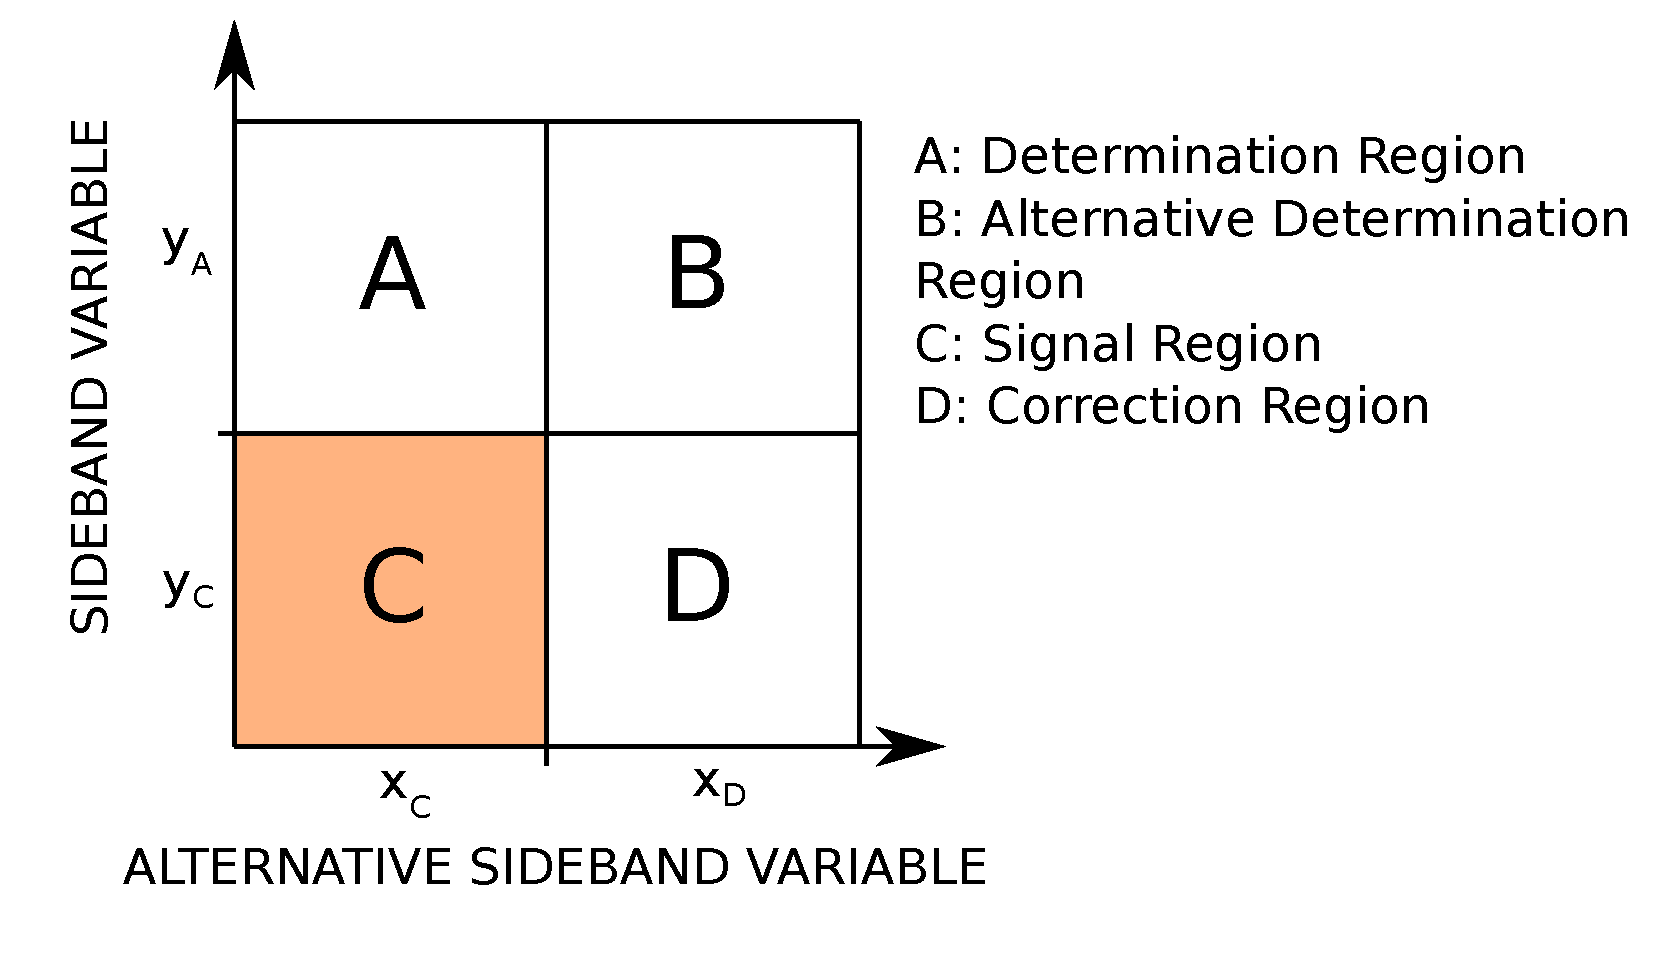
\includegraphics[width=0.8\textwidth]{Figures/ff_diagram_v2.pdf}
\caption{Schematic of the regions used for fake factor derivation.}
\label{fig:ff_schematic}
\end{figure}

Region A is used to measure and fit fake factors.
Region B is an alternative region used to measure and fit fake factor to account for the difference in fake factors between A and C.
These alternative fake factors are applied to the fail region in D and corrections are calculated comparing it to the pass region in D.
The total fake factor per measurement region is calculated as the fake factors derived in region A multiplied by the correction calculated from region B to D. \\

The selection for $x_C$, $x_D$, $y_C$ and $y_A$, as defined in Figure~\ref{fig:ff_schematic}, in each separate measurement region are shown below.
These are chosen to balance the number of events and the purity of each background in the region.

\begin{enumerate}[i)]
   \item $\tauhtauh$ QCD \\
     \indent $y_C$: The $\tauh$ candidates are required to have the opposite sign. \\
     \indent $y_A$: The $\tauh$ candidates are required to have the same sign. \\
     \indent $x_C$: The subleading tau passes the \texttt{Medium} $D_{\text{jet}^{\text{WP}}}$. \\
     \indent $x_D$: The subleading tau fails the \texttt{VVLoose} $D_{\text{jet}^{\text{WP}}}$ but passes the \texttt{VVVLoose} $D_{\text{jet}^{\text{WP}}}$.
  \item $\etauh$ and $\mutauh$ QCD \\
    \indent $y_C$: The $e$/$\mu$ and $\tauh$ candidates are required to have the opposite sign. \\
    \indent $y_A$: The $e$/$\mu$ and $\tauh$ candidates are required to have the same sign and the $e$/$\mu$ to have $\Irel>0.05$. \\
    \indent $x_C$: The $e$/$\mu$ candidate is required to have $\Irel<0.15$. \\
    \indent $x_D$: The $e$/$\mu$ candidate is required to have $0.25<\Irel<0.5$.
  \item $\etauh$ and $\mutauh$ W + Jets \\
    \indent $y_C$: The $\mT$ between the $e$/$\mu$ and the MET $< 70$ GeV. \\
    \indent $y_A$: The $\mT$ between the $e$/$\mu$ and the MET $> 70$ GeV and no b jets in the event. \\
    \indent $x_C$: Data. \\
    \indent $x_D$: W + Jets MC.
  \item $\etauh$ and $\mutauh$ $\ttbar$ \\
    \indent $y_C$: Data. \\
    \indent $y_A$: MC ($\ttbar$ in B and W + Jets D). \\
    \indent $x_C$: $\mT < 70$ GeV. \\
    \indent $x_D$: $\mT > 70$ GeV and no b jets. \\
\end{enumerate}


In the $\mu\tauh$ and $e\tauh$ channels QCD and W + Jets jet fake events are in general the most significant and contribute with approximately equal weights. 
$\ttbar$ inclusively is small but becomes more significant when searching for events with a b jet. 
The additional $\Irel>0.05$ requirement in these channels for QCD is to reduce processes producing genuine leptons and the $N_{\text{b-jets}}=0$ requirement for W + Jets is to reduce $\ttbar$ contamination.
It is not possible to define a DR that is sufficiently pure in $\ttbar$ events to make a reasonable measurement of $\FF^{\ttbar}$ from data.
Therefore $\FF^{\ttbar}$ are derived from MC. 
A comparison of the $\FF^{\text{W+jets}}$ measured in data and MC shows only $\sim$ 10--20\% differences in the fake rates in data and MC.  
This observation coupled with the fact that the $\ttbar$ contribution is small compared to the other processes means that any bias introduced by using $\FF^{\ttbar}$ measured in MC is small compared to the uncertainties on the fake factors, discussed in Section~\ref{sec:uncertainties}. \\


\subsection{Parametrisation}

The $\FFi$ take into account dependencies on $N_{\text{jets}}$ via the analysis tailed variable $N_{\text{pre b-jets}}$, the $\pT$ of the $\tauh$ candidate ($\pT^{\tauh}$) and the $\pT$ of the jet matched in $\Delta R$ to the $\tauh$ ($\pT^{\text{jet}}$).
$N_{\text{pre b-jets}}$ is defined to map the dependence of $\FFi$ on $N_{\text{jets}}$ and describe the categorising variable $N_{\text{b-jets}}$ well.
It is the number of jets in the event with $|\eta|<2.4$ and $\pT>20$. These are the same $\eta$ and $\pT$ thresholds required for a b-jet.
They are also calculated separately for the three channels where a jet can fake a hadronic tau, $e\tauh$, $\mu\tauh$ and $\tauh\tauh$.
The $\FFi$ are then measured separately for the dominant $\text{jet}\rightarrow\tauh$ processes $\text{i}$, which for the $e\tauh$ and $\mu\tauh$ channels includes QCD, W+jets and $t\bar{t}r$, and for the $\tauh\tauh$ channel includes only QCD.
The $\FFi$ are finally corrected to account for extrapolations from the DR to the SR, and for missing variable dependencies (via non-closure corrections).
The $\FFi$ measured for the different processes are combined into an overall factor, $\FF$, using
\begin{equation}
\FF = \sum_{i}f_{i}\cdot \FFi,
\end{equation}
where the factor $f_{i}$ is defined as
\begin{equation}
f_{i} = \frac{N_{\text{AR}}^{i}}{\sum\limits_{j}N_{\text{AR}}^{j}},
\end{equation}
which is the fraction of events with a $\text{jet}\rightarrow\tauh$ originating from process $i$ over the total number of $\text{jet}\rightarrow\tauh$ events for all processes in the AR.

\begin{figure}[!hbtp]
\centering
    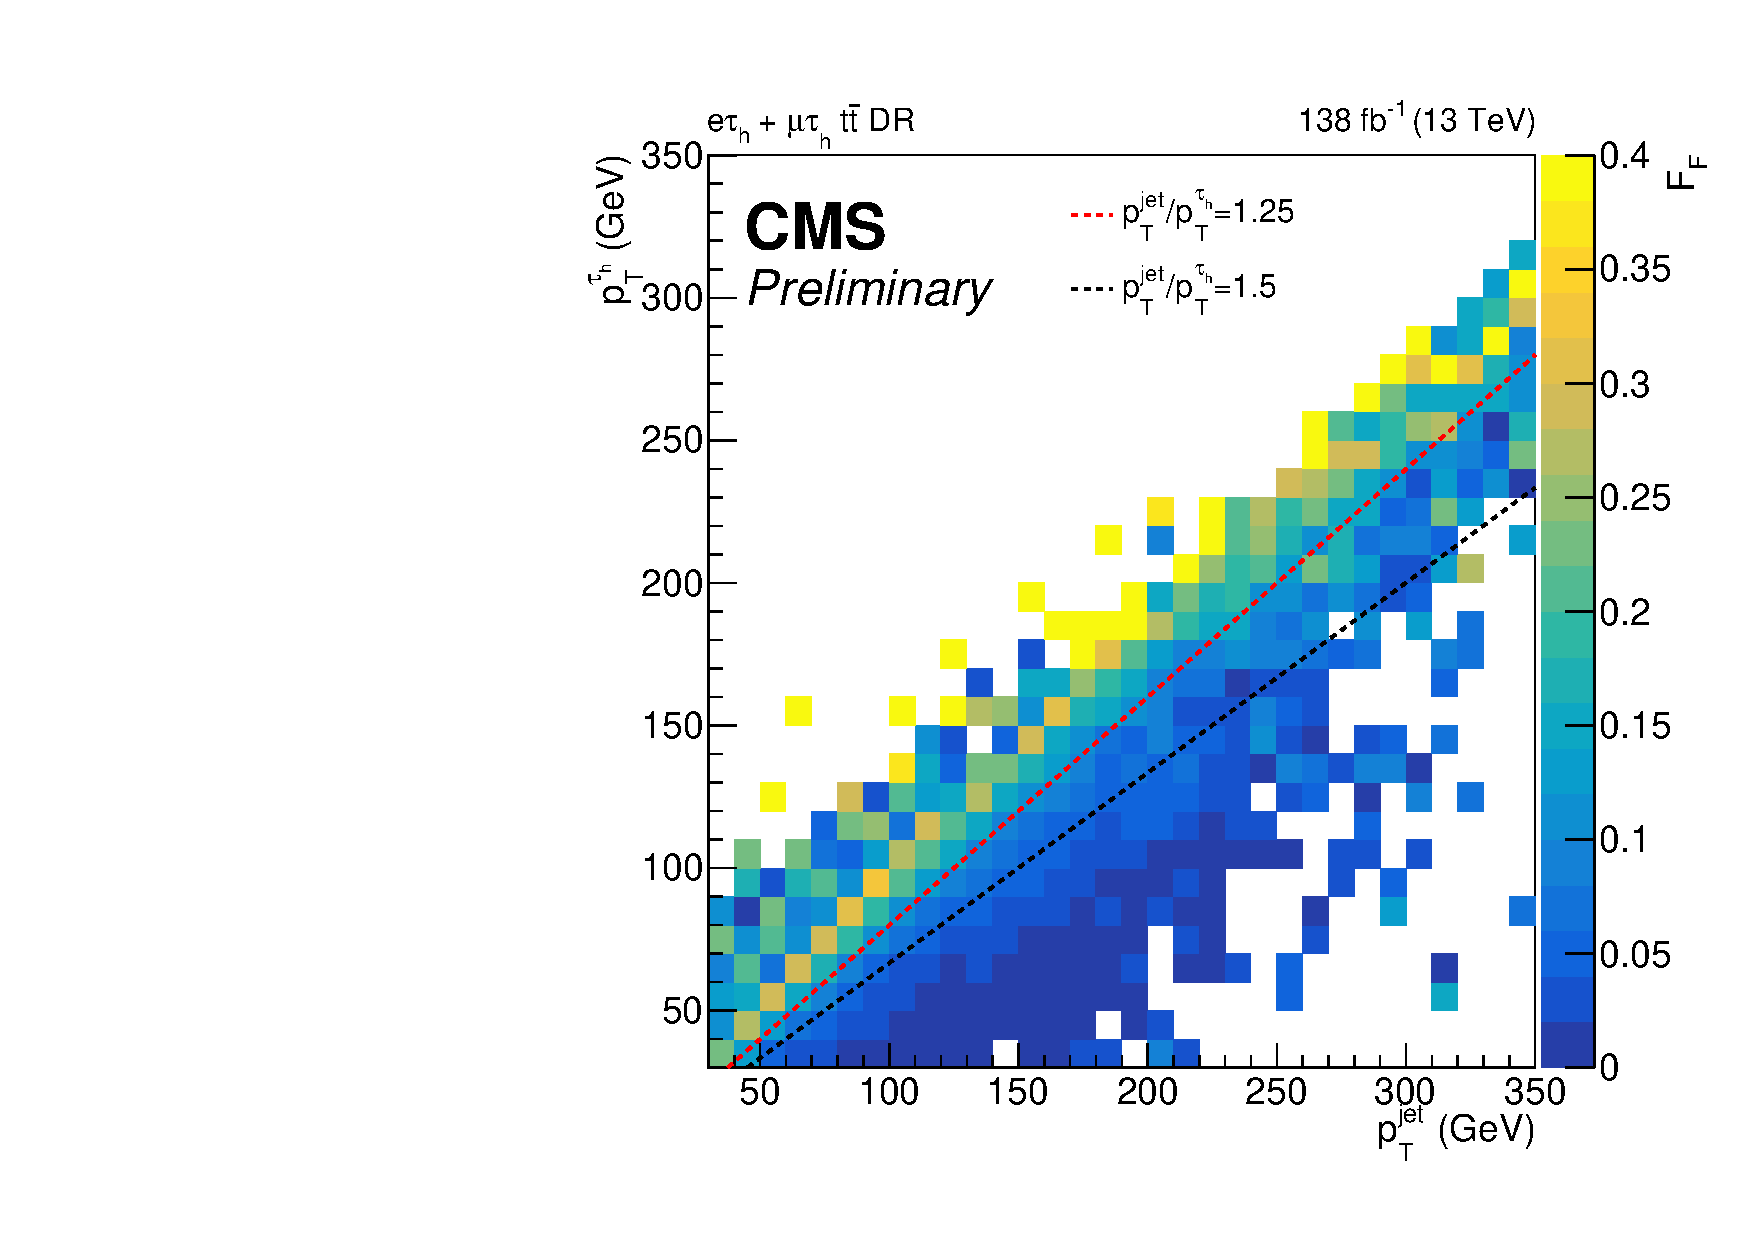
\includegraphics[width=0.6\textwidth]{Figures/ff_colz_ttbar_lt.pdf}
\caption{A 2D heat map of the fake factors determined from $t\bar{t}$ MC for the full run-2 dataset in the combined $e\tauh$ and $\mu\tauh$ channels. This is shown with respect to the hadronic tau $\pT$ and the $\pT$ of the jet matched to the hadronic tau. The ratio of jet to hadronic tau $\pT$ categorisation used is shown split by the dashed lines.}
\label{fig:ff_colz}
\end{figure}

\begin{figure}[!hbtp]
\centering
    \subfloat[]{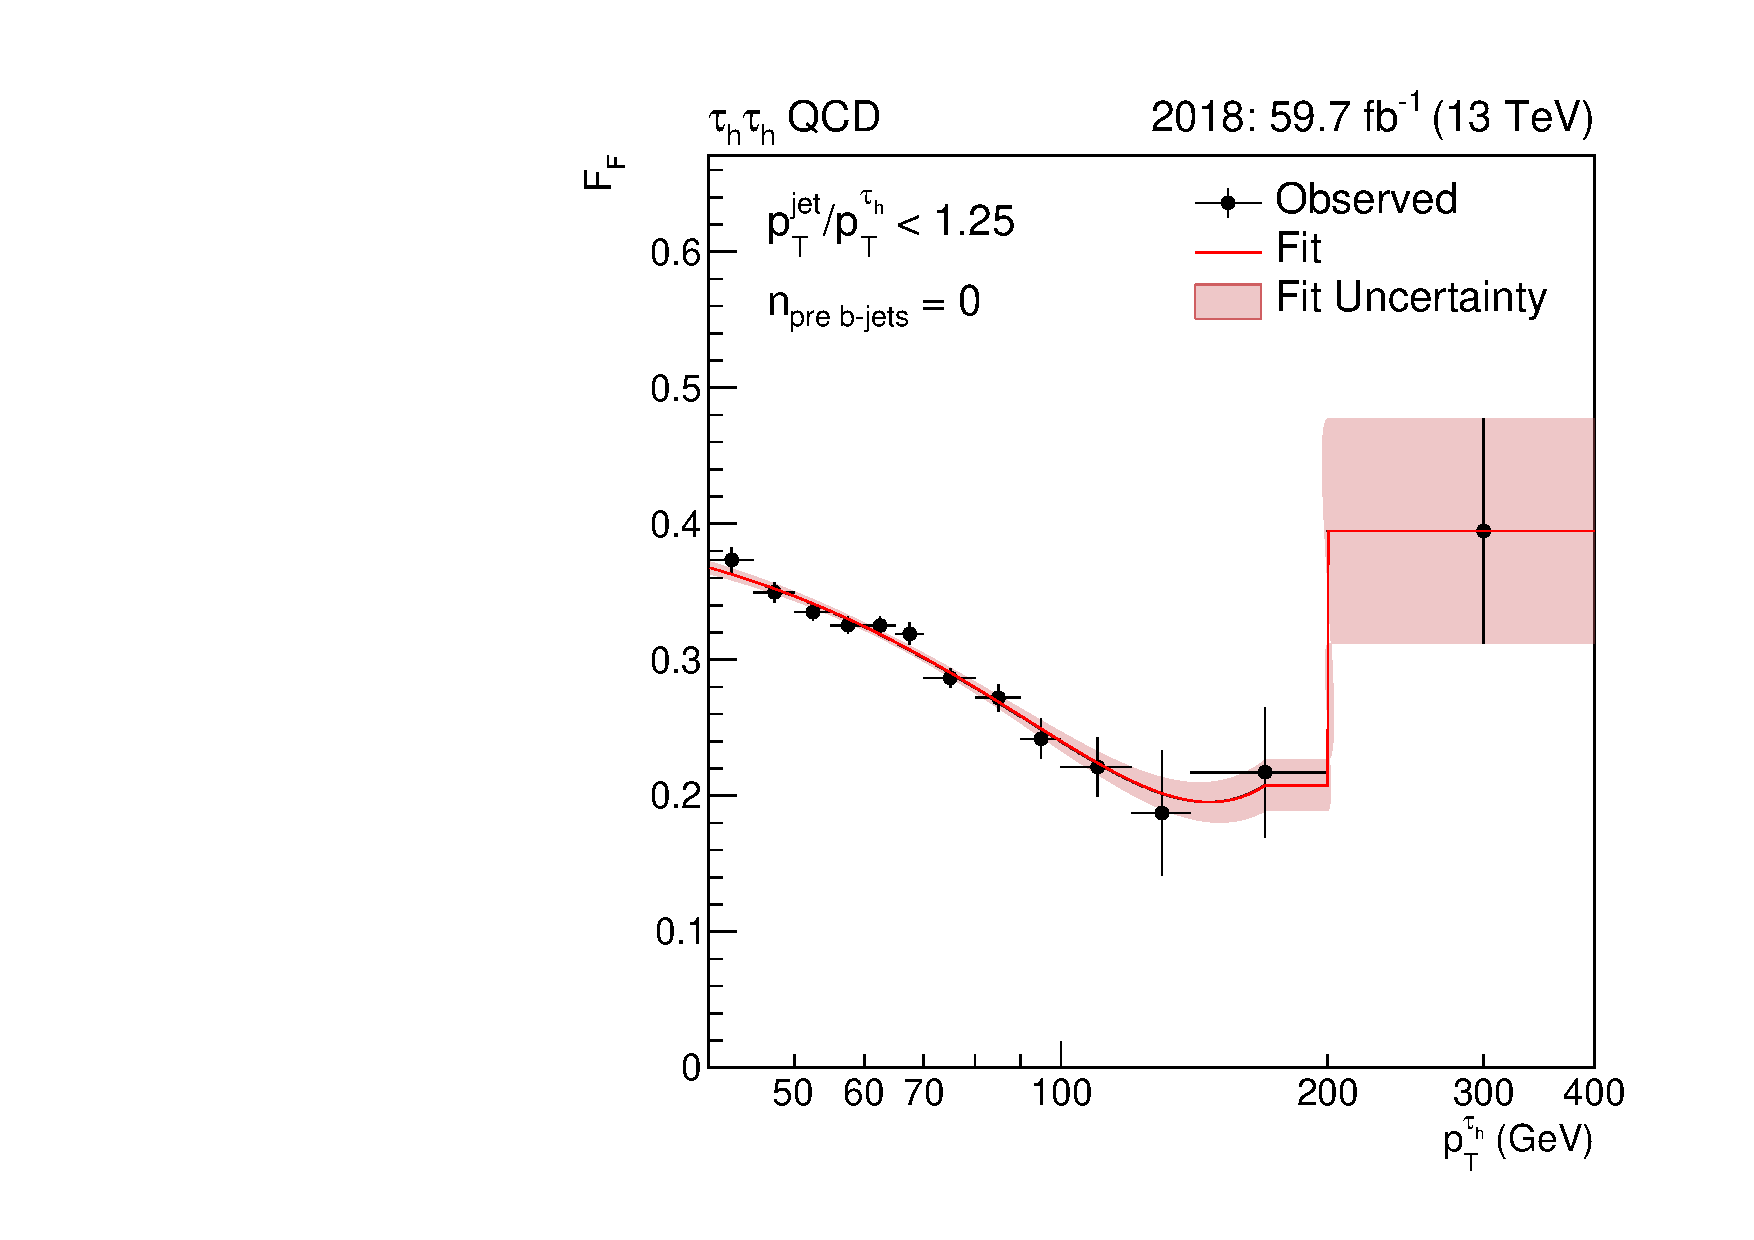
\includegraphics[width=0.33\textwidth]{Figures/ff_fit_jet_pt_low_0jet_pt_1_ff_qcd_tt_2018.pdf}}
    \subfloat[]{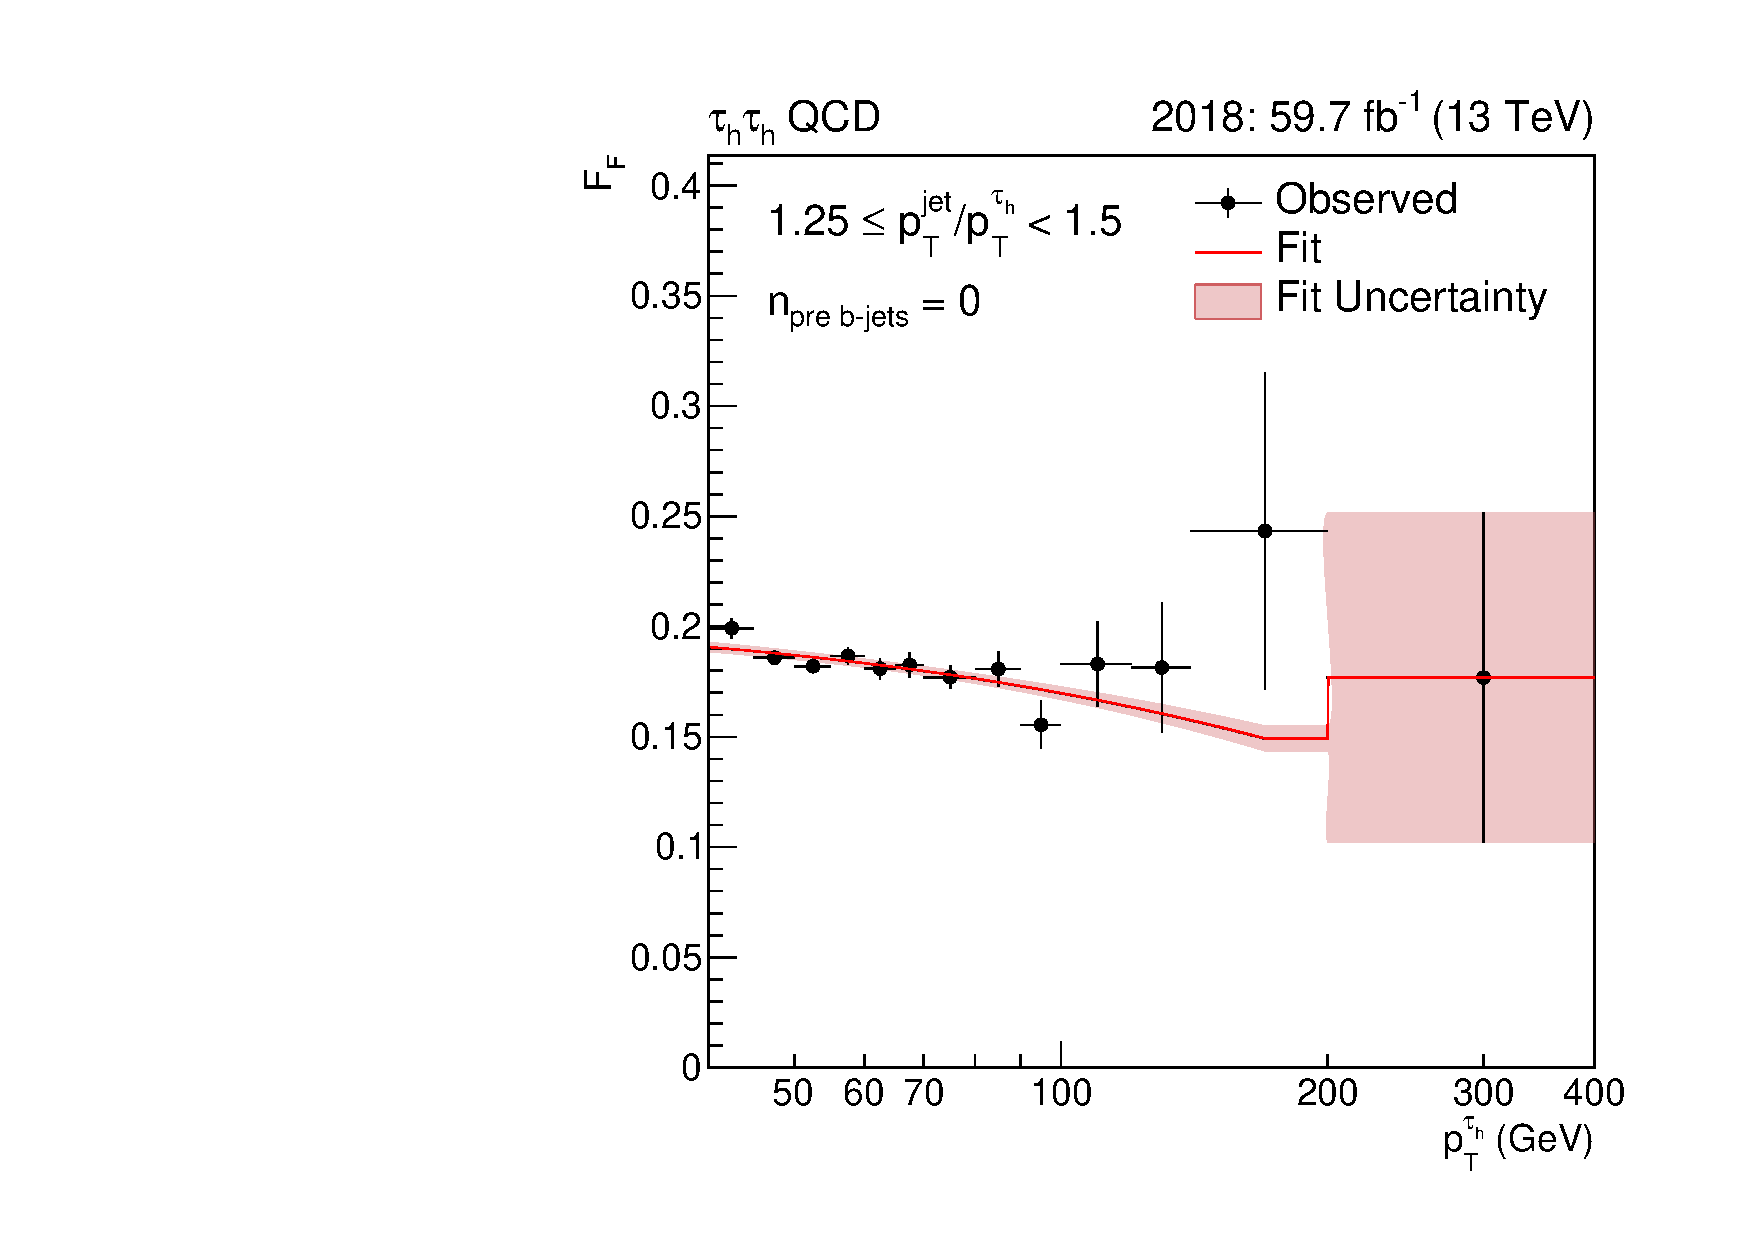
\includegraphics[width=0.33\textwidth]{Figures/ff_fit_jet_pt_med_0jet_pt_1_ff_qcd_tt_2018.pdf}} 
    \subfloat[]{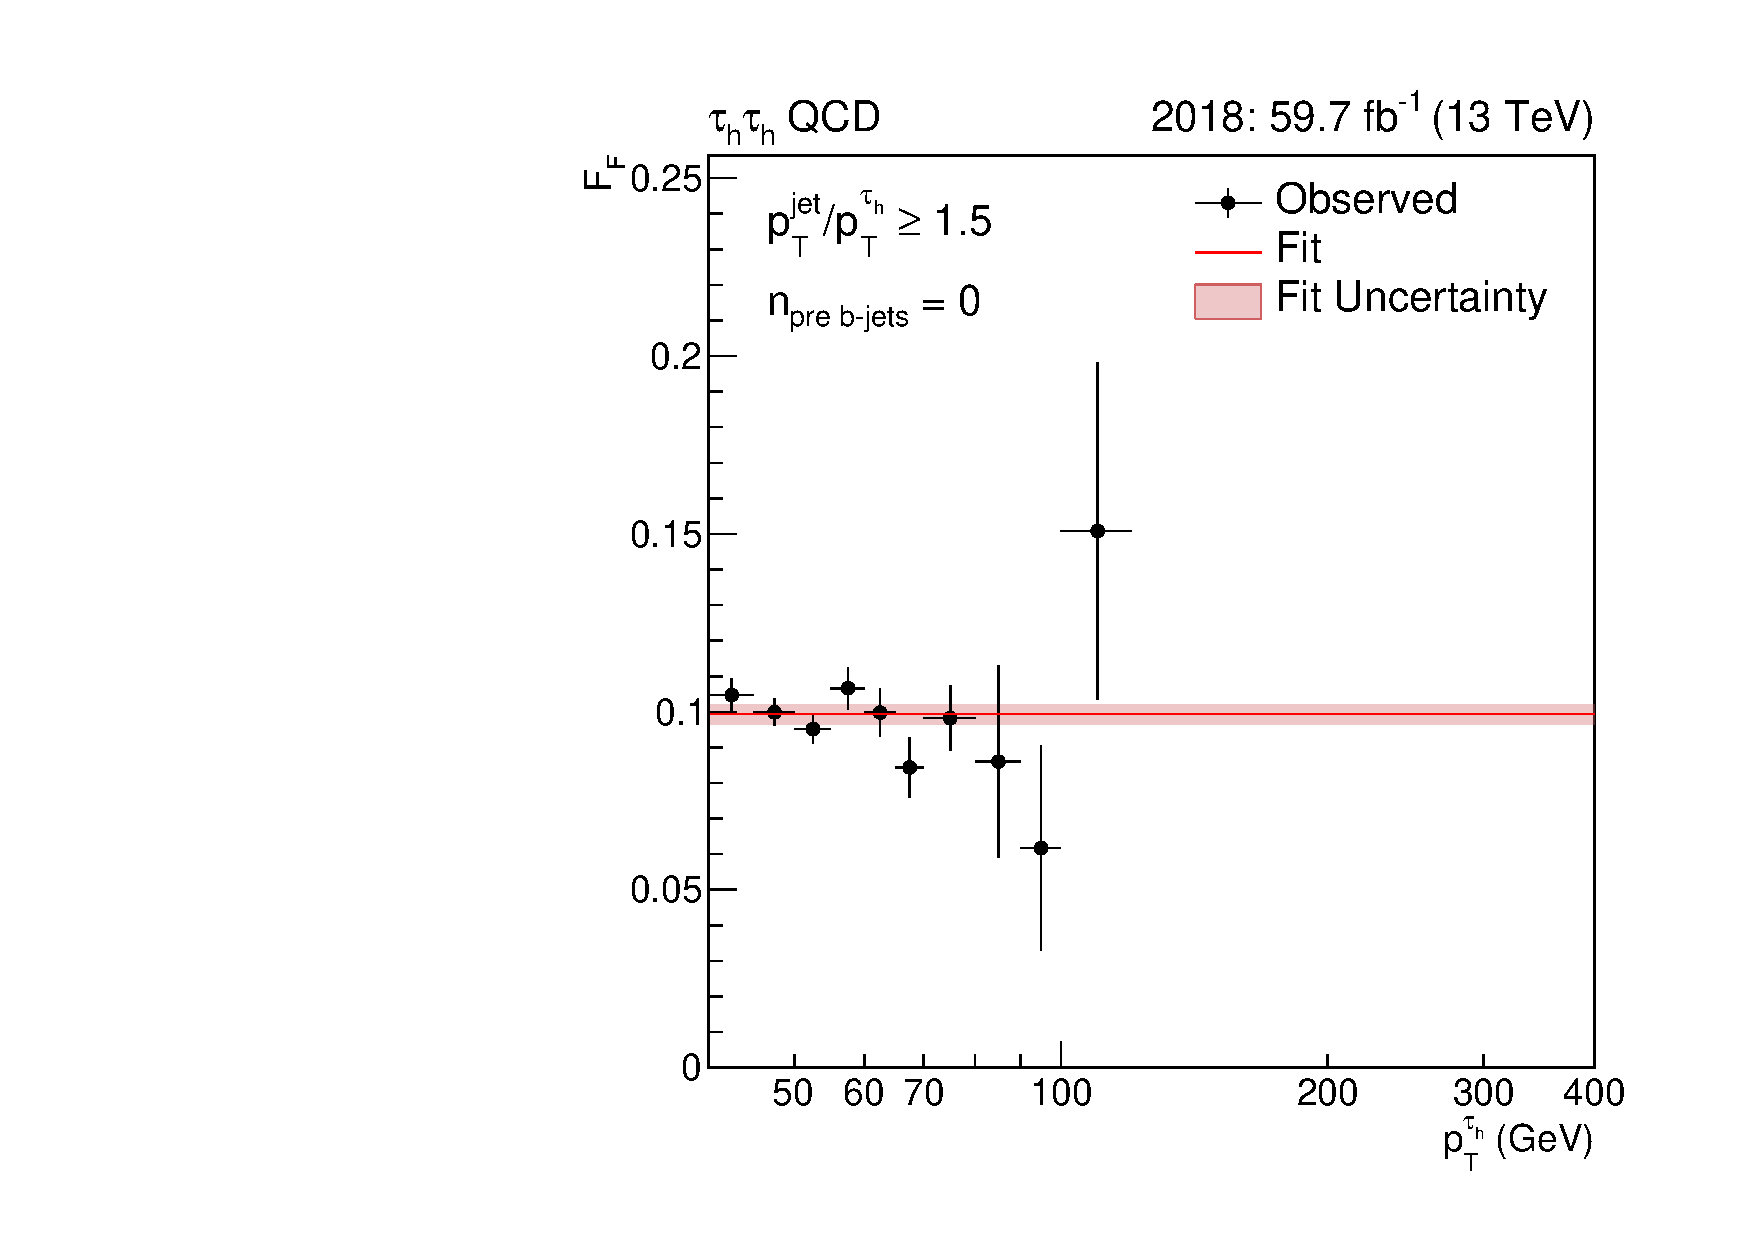
\includegraphics[width=0.33\textwidth]{Figures/ff_fit_jet_pt_high_0jet_pt_1_ff_qcd_tt_2018.pdf}} \\
\caption{Fake factor fits in $\tauh\tauh$ channel for the QCD $n_{pre b jets}=0$ category with 2018 data. The three jet $\pT$ to hadronic tau $\pT$ categories are shown.}
\label{fig:tt_ff_fit}
\end{figure}

\begin{figure}[!hbtp]
\centering
    \subfloat[]{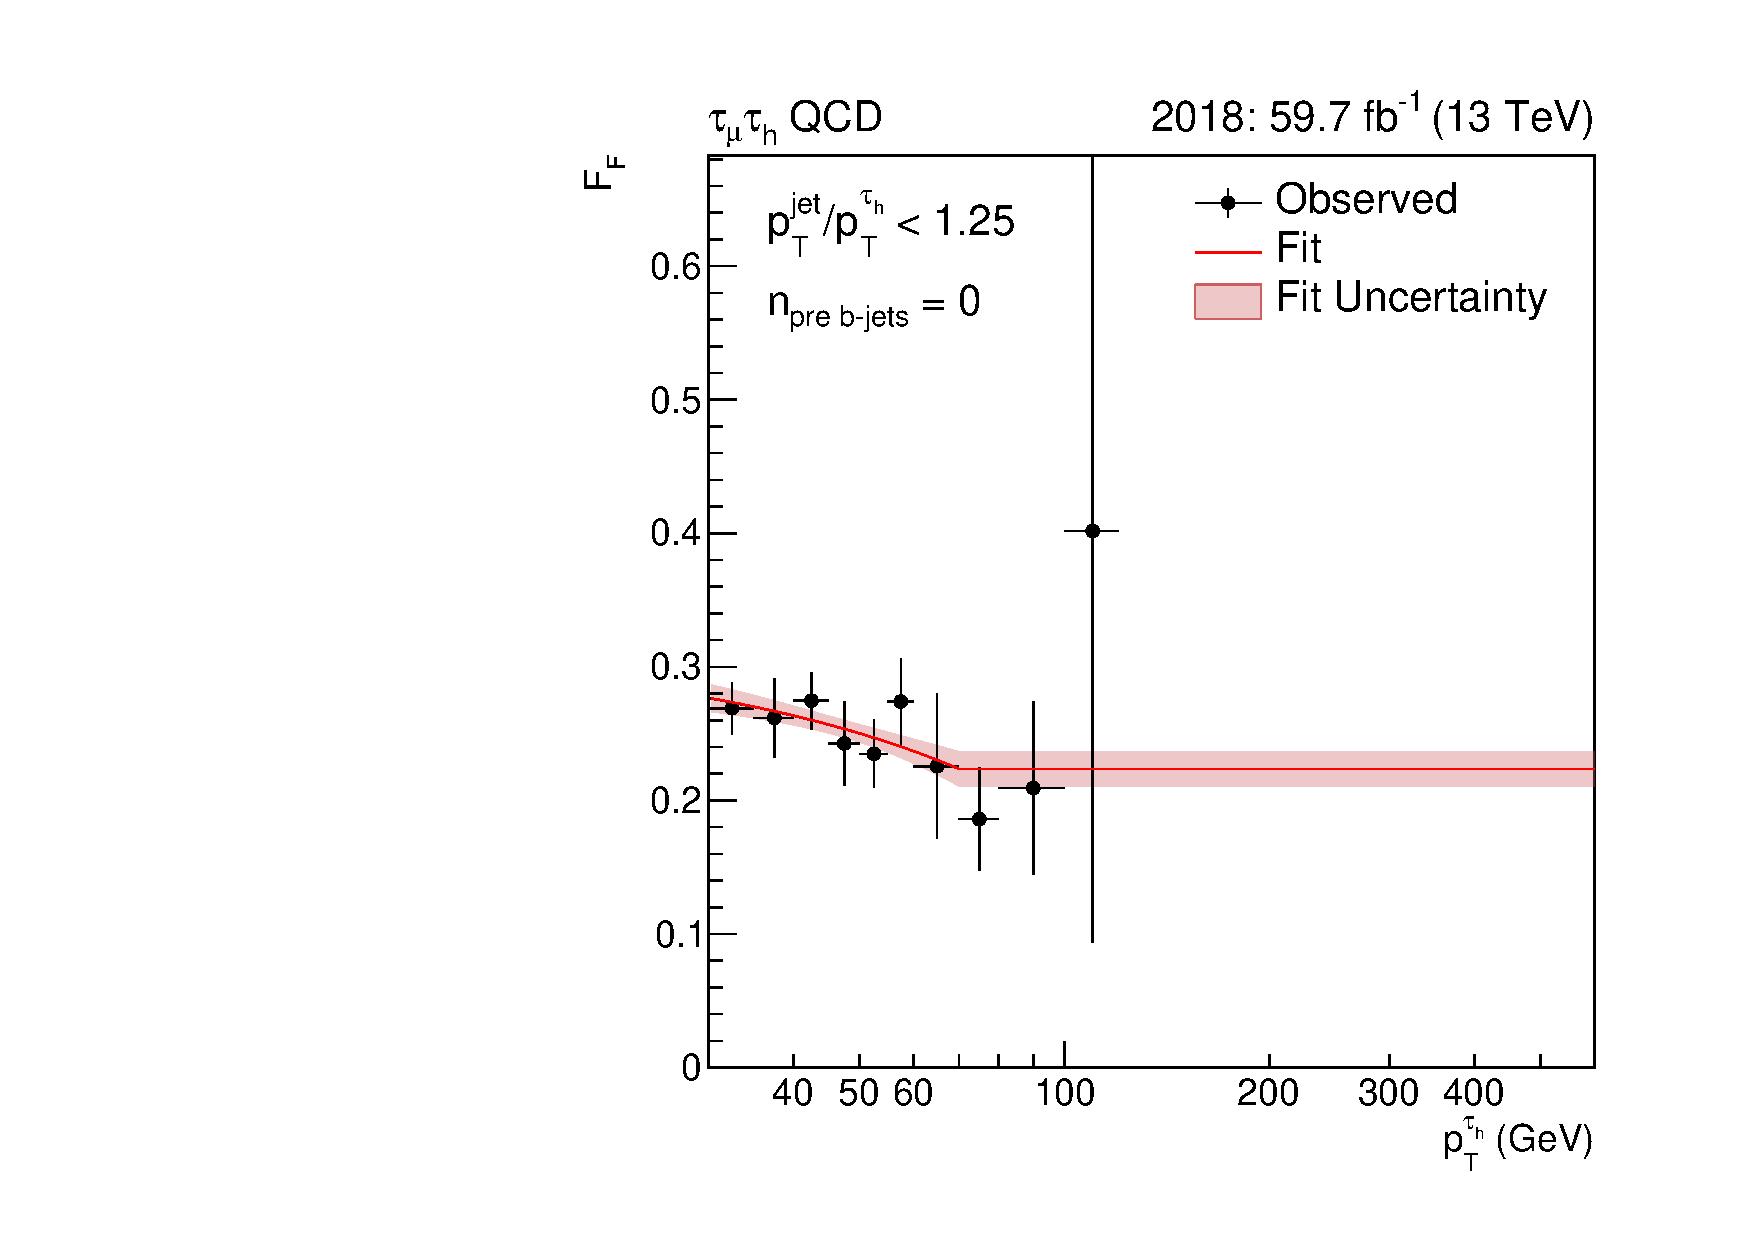
\includegraphics[width=0.33\textwidth]{Figures/ff_fit_jet_pt_low_0jet_pt_2_ff_qcd_mt_2018.pdf}}
    \subfloat[]{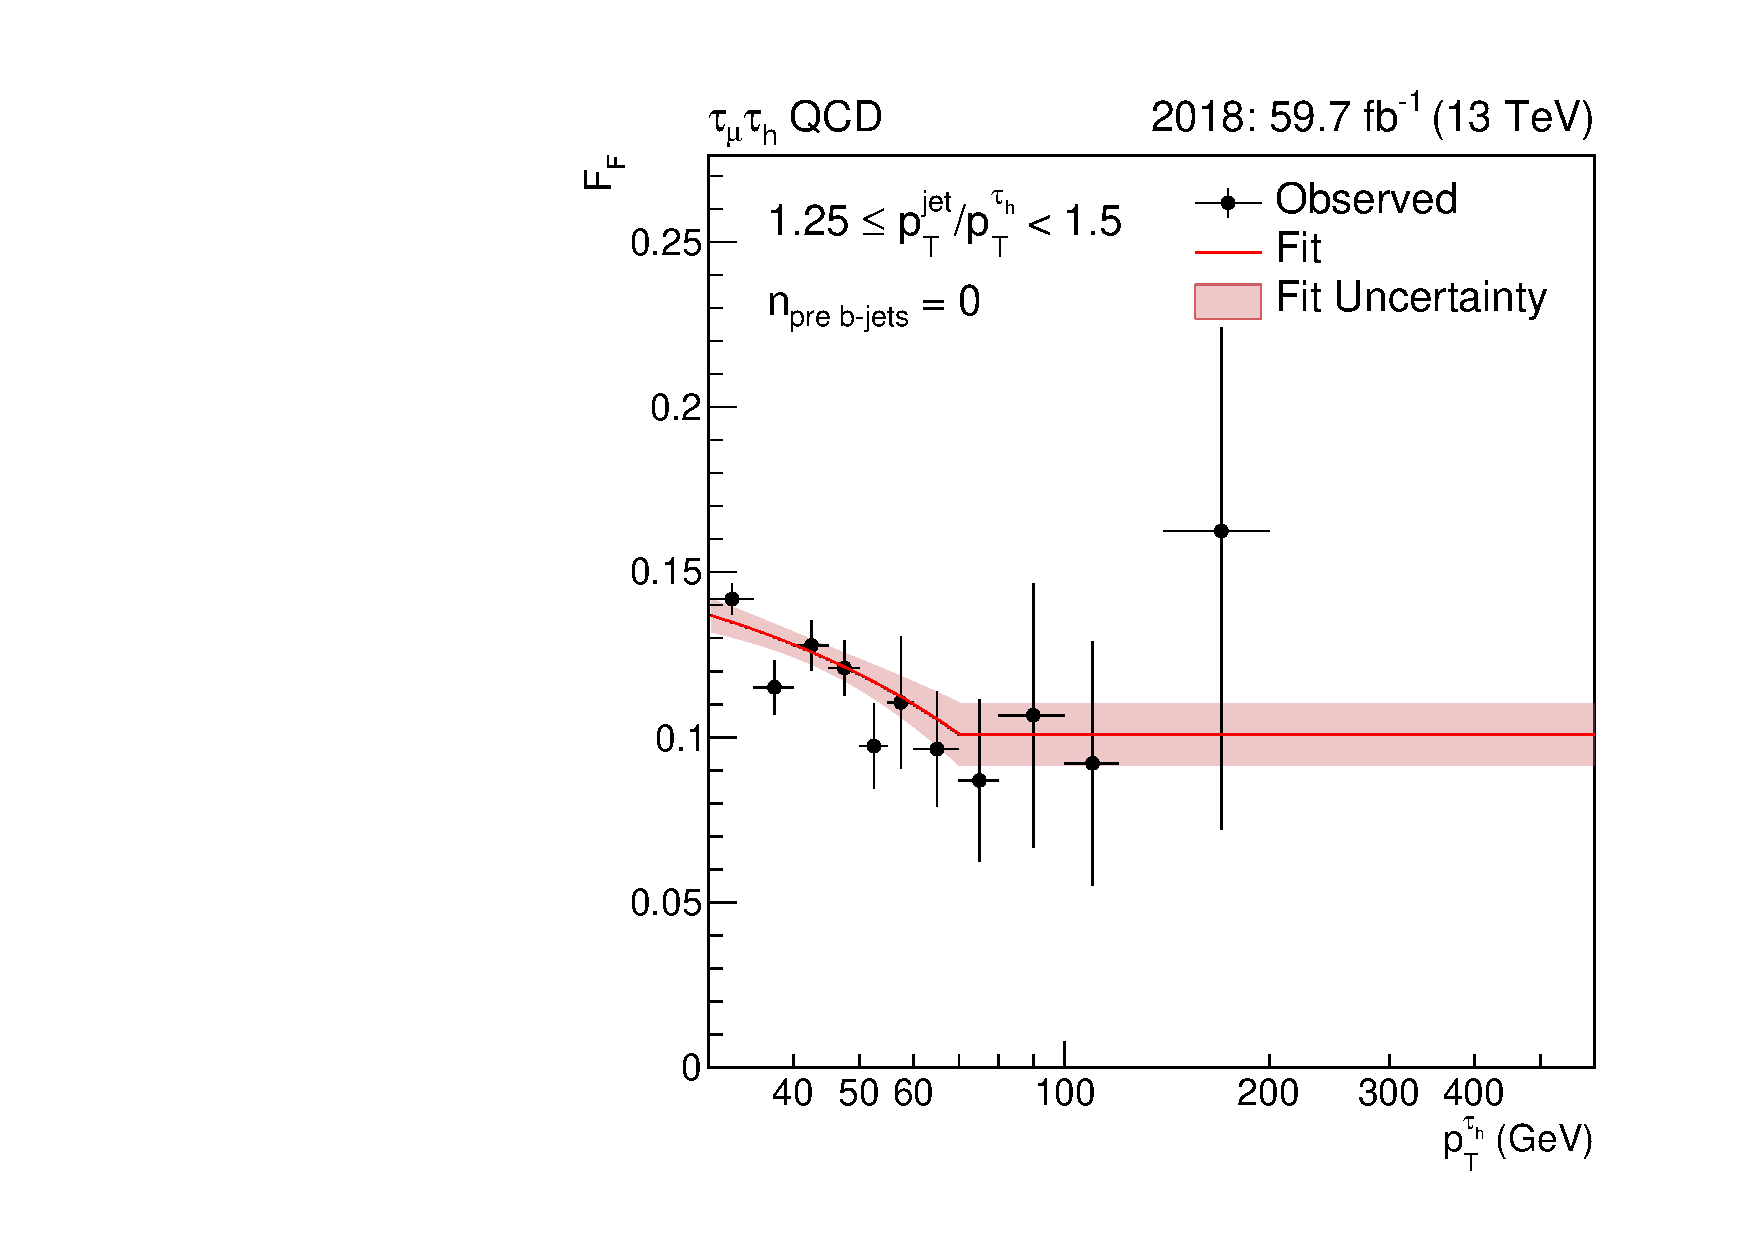
\includegraphics[width=0.33\textwidth]{Figures/ff_fit_jet_pt_med_0jet_pt_2_ff_qcd_mt_2018.pdf}} 
    \subfloat[]{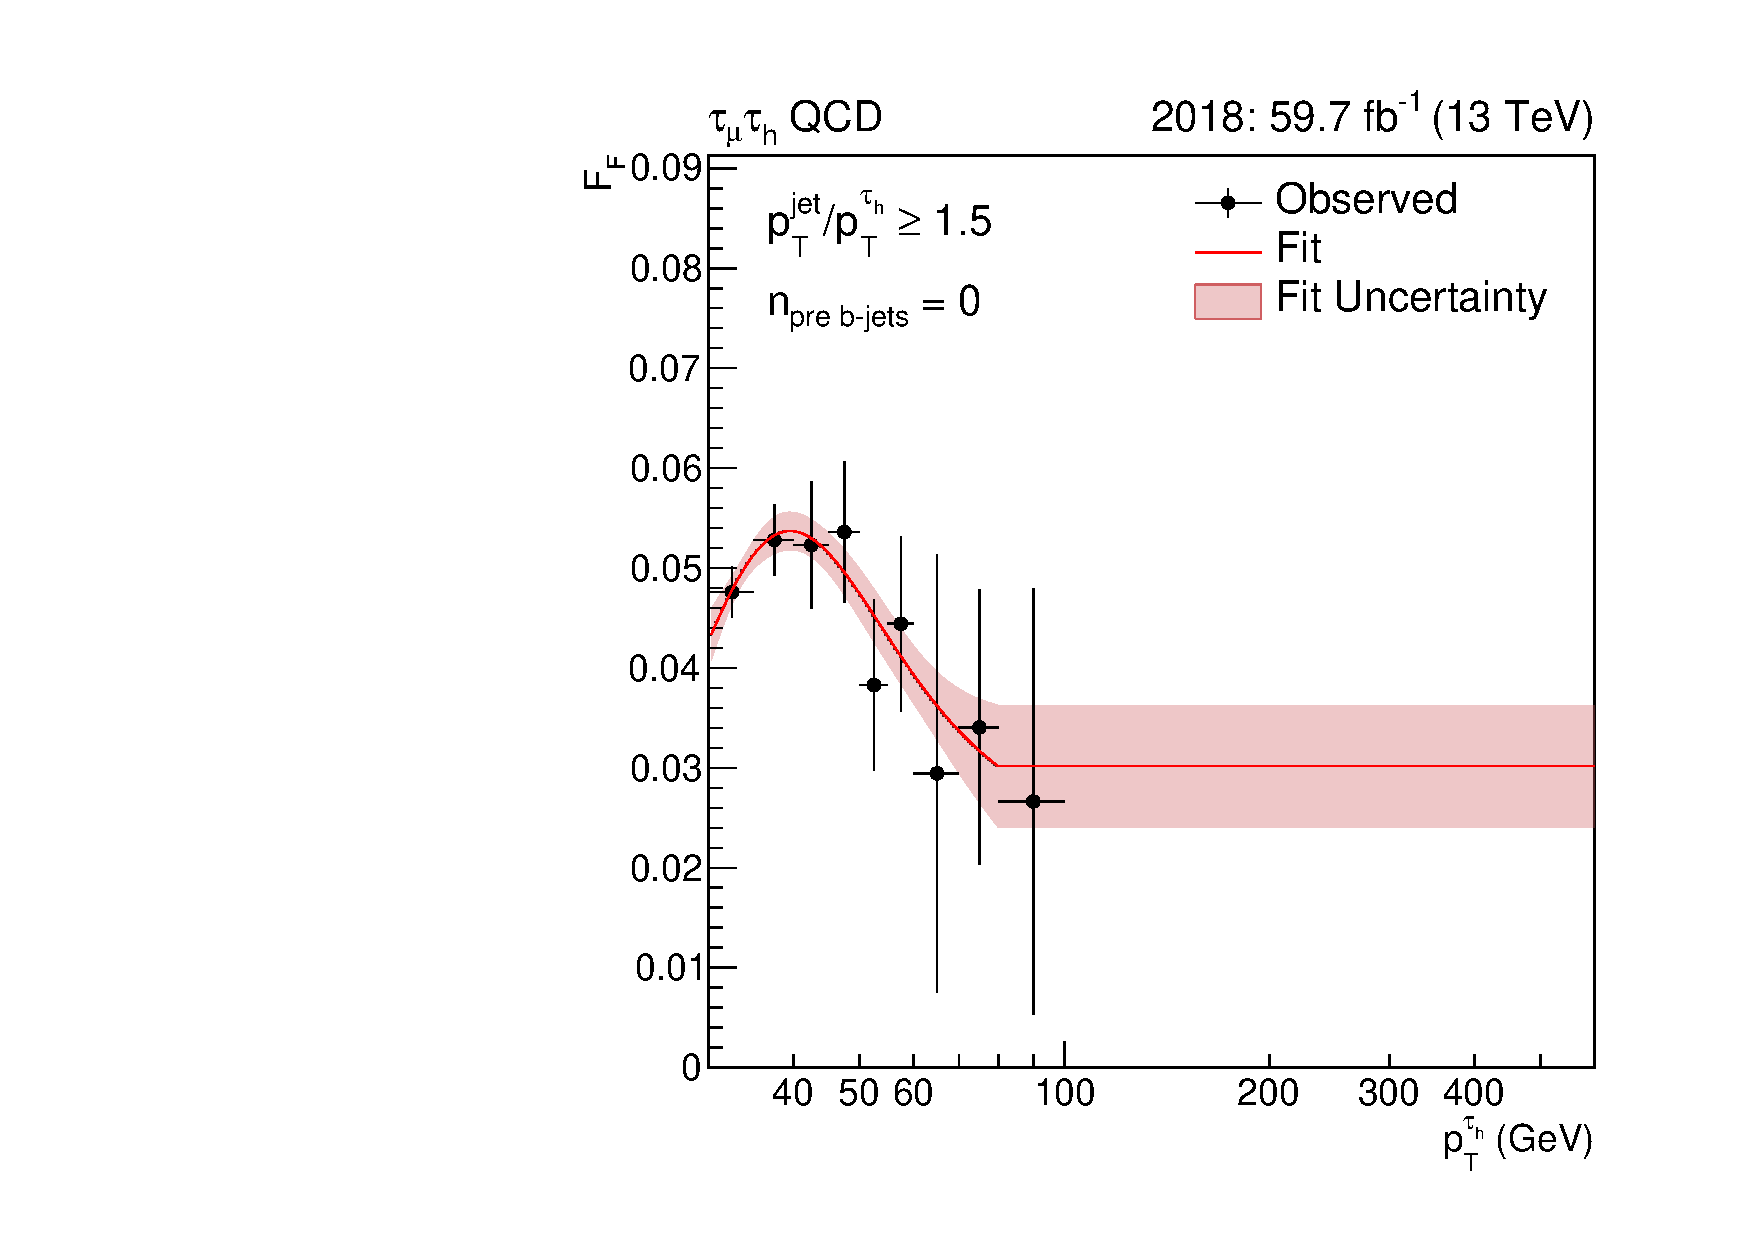
\includegraphics[width=0.33\textwidth]{Figures/ff_fit_jet_pt_high_0jet_pt_2_ff_qcd_mt_2018.pdf}} \\
    \subfloat[]{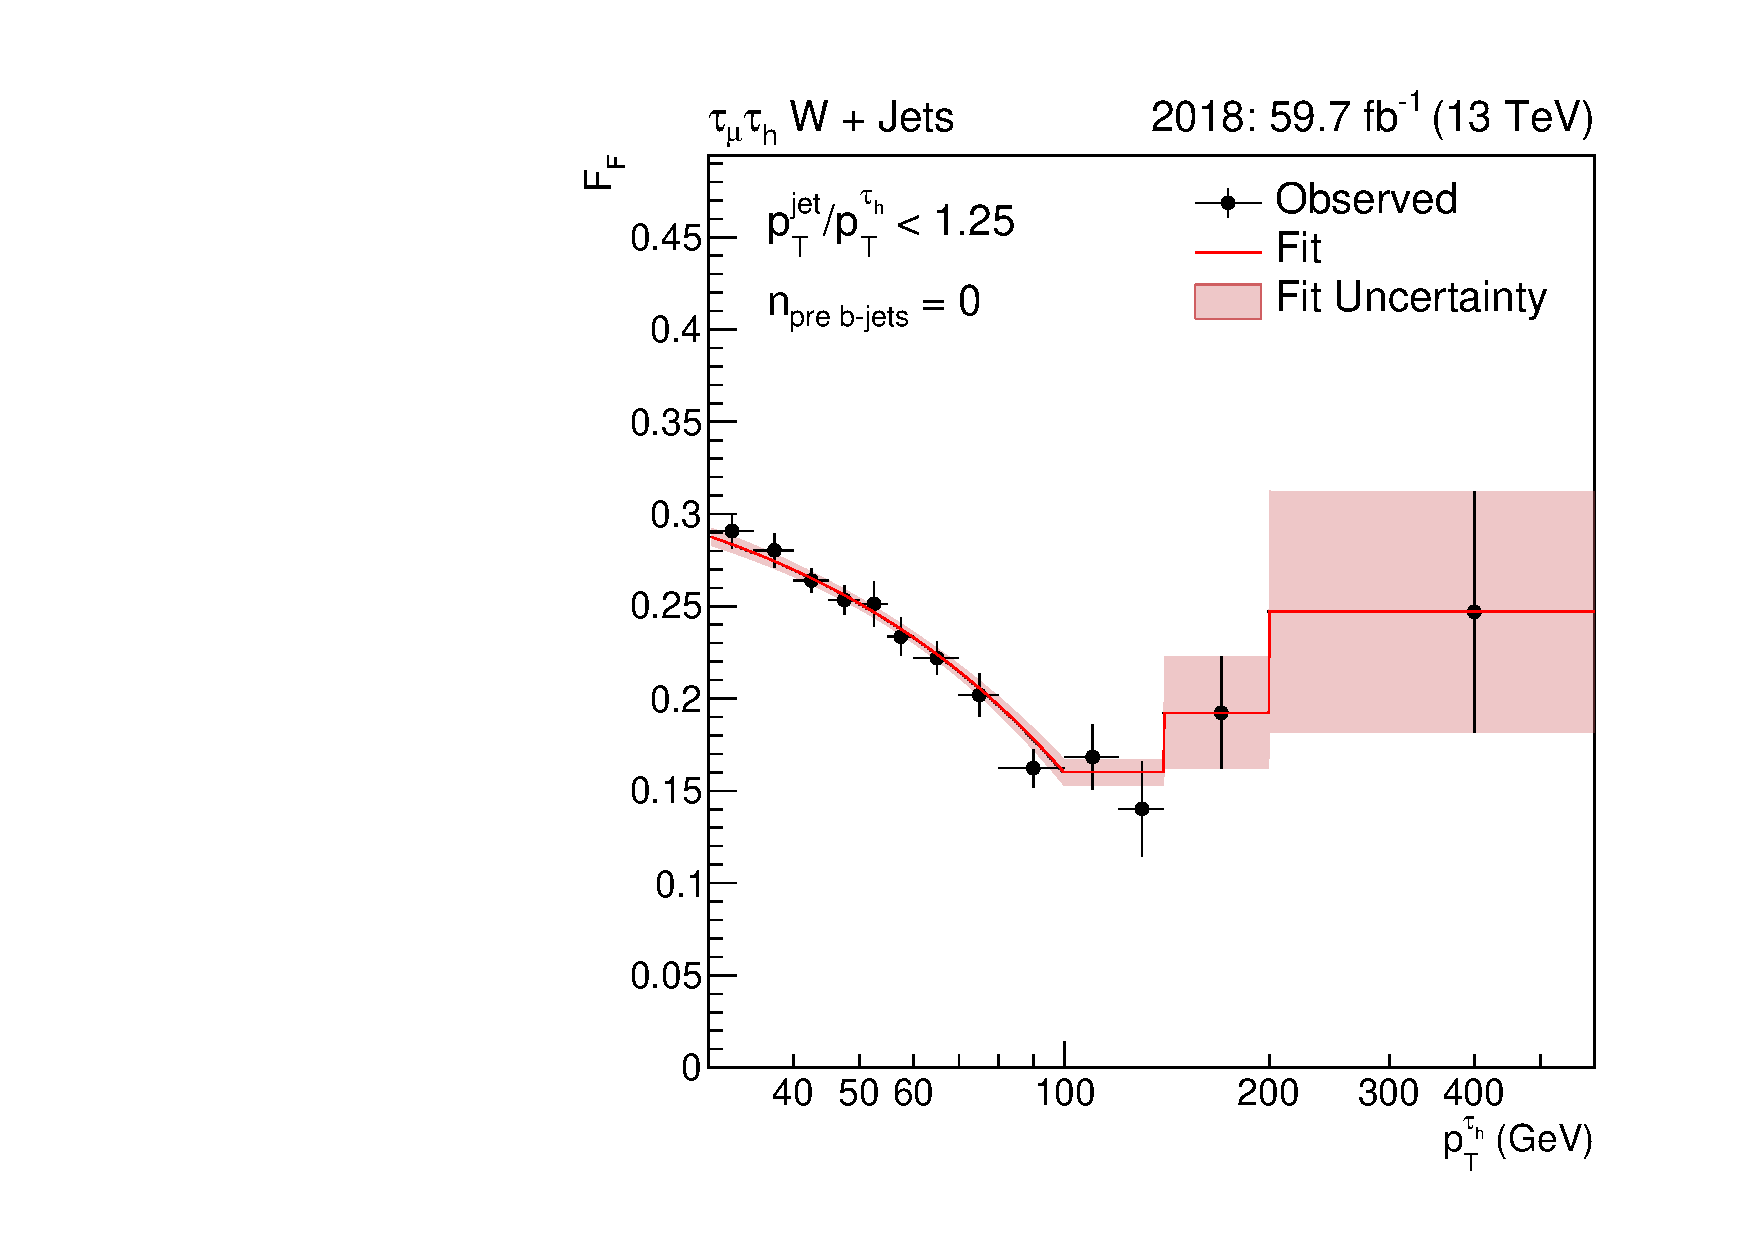
\includegraphics[width=0.33\textwidth]{Figures/ff_fit_jet_pt_low_0jet_pt_2_ff_wjets_mt_2018.pdf}}
    \subfloat[]{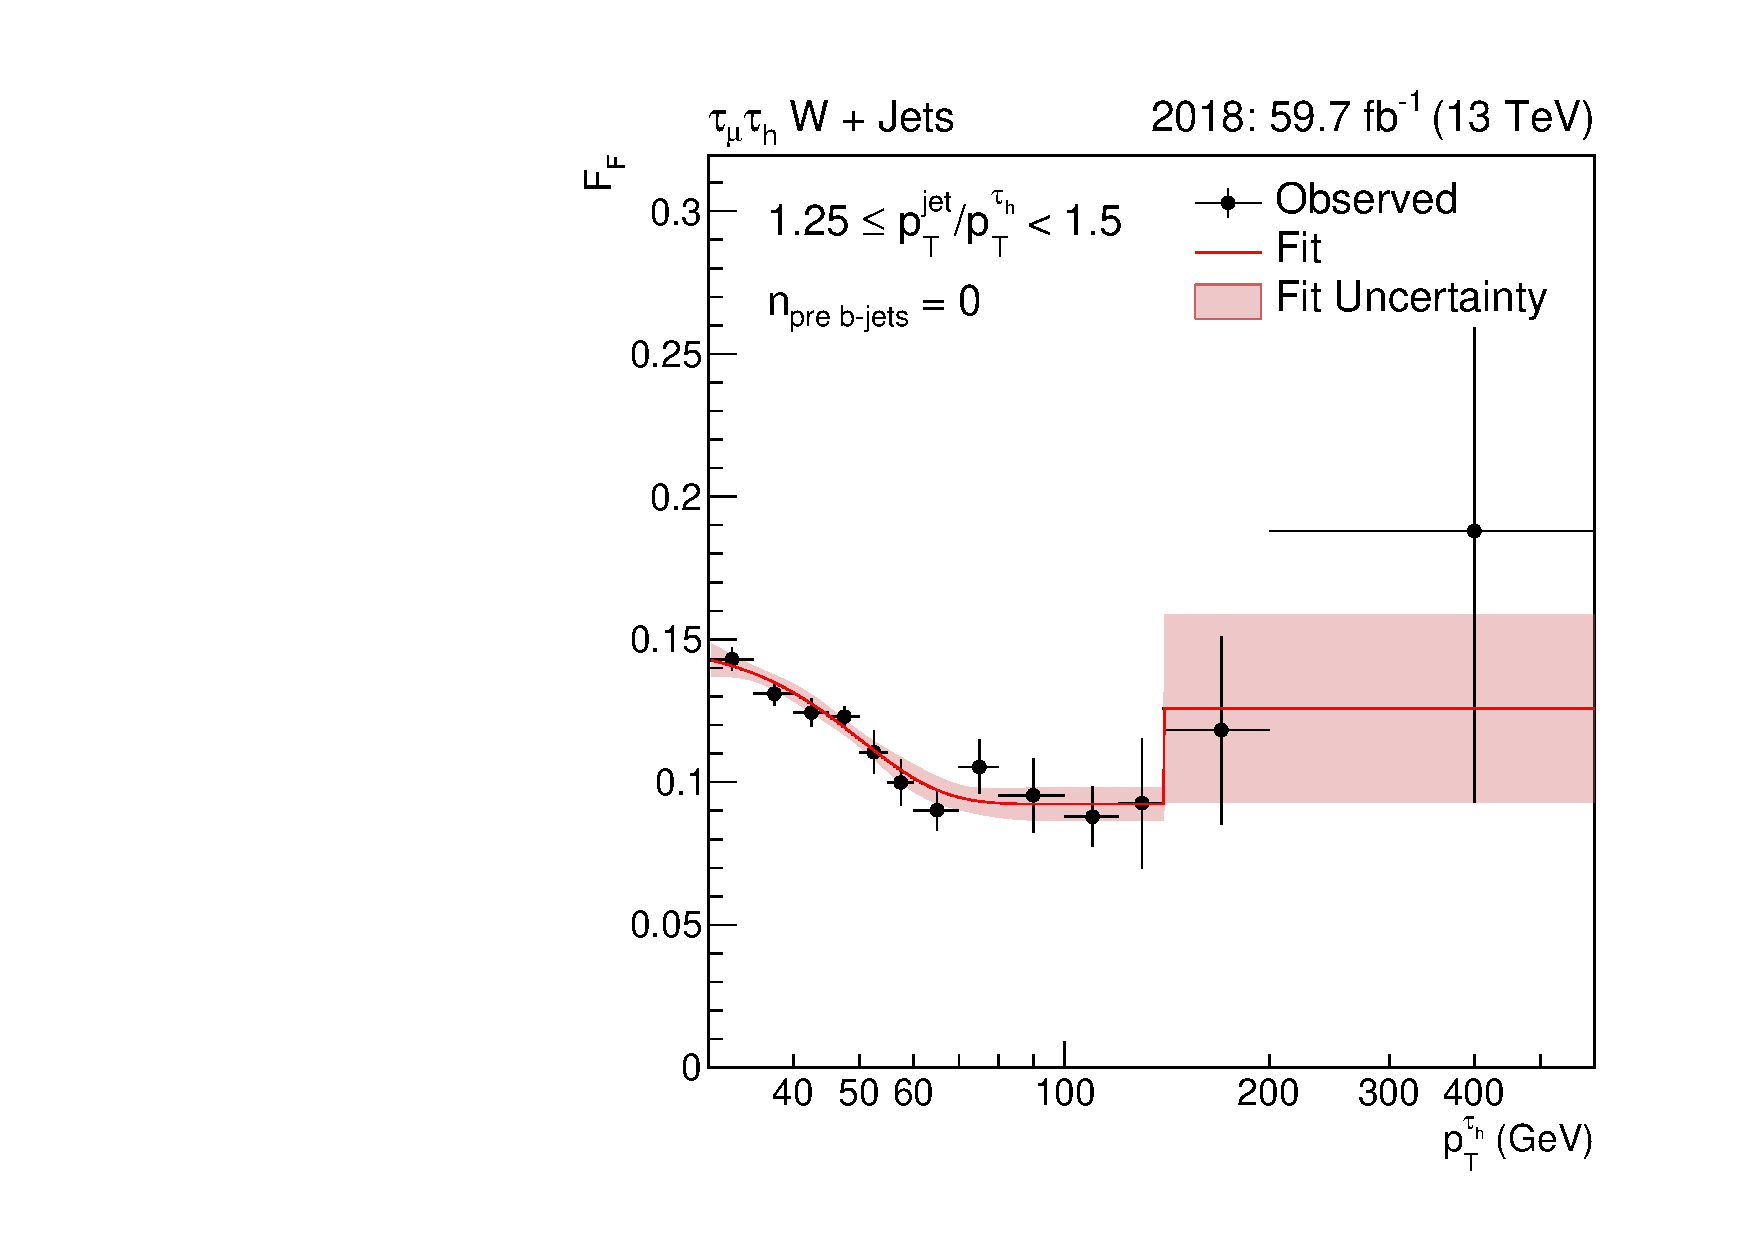
\includegraphics[width=0.33\textwidth]{Figures/ff_fit_jet_pt_med_0jet_pt_2_ff_wjets_mt_2018.pdf}} 
    \subfloat[]{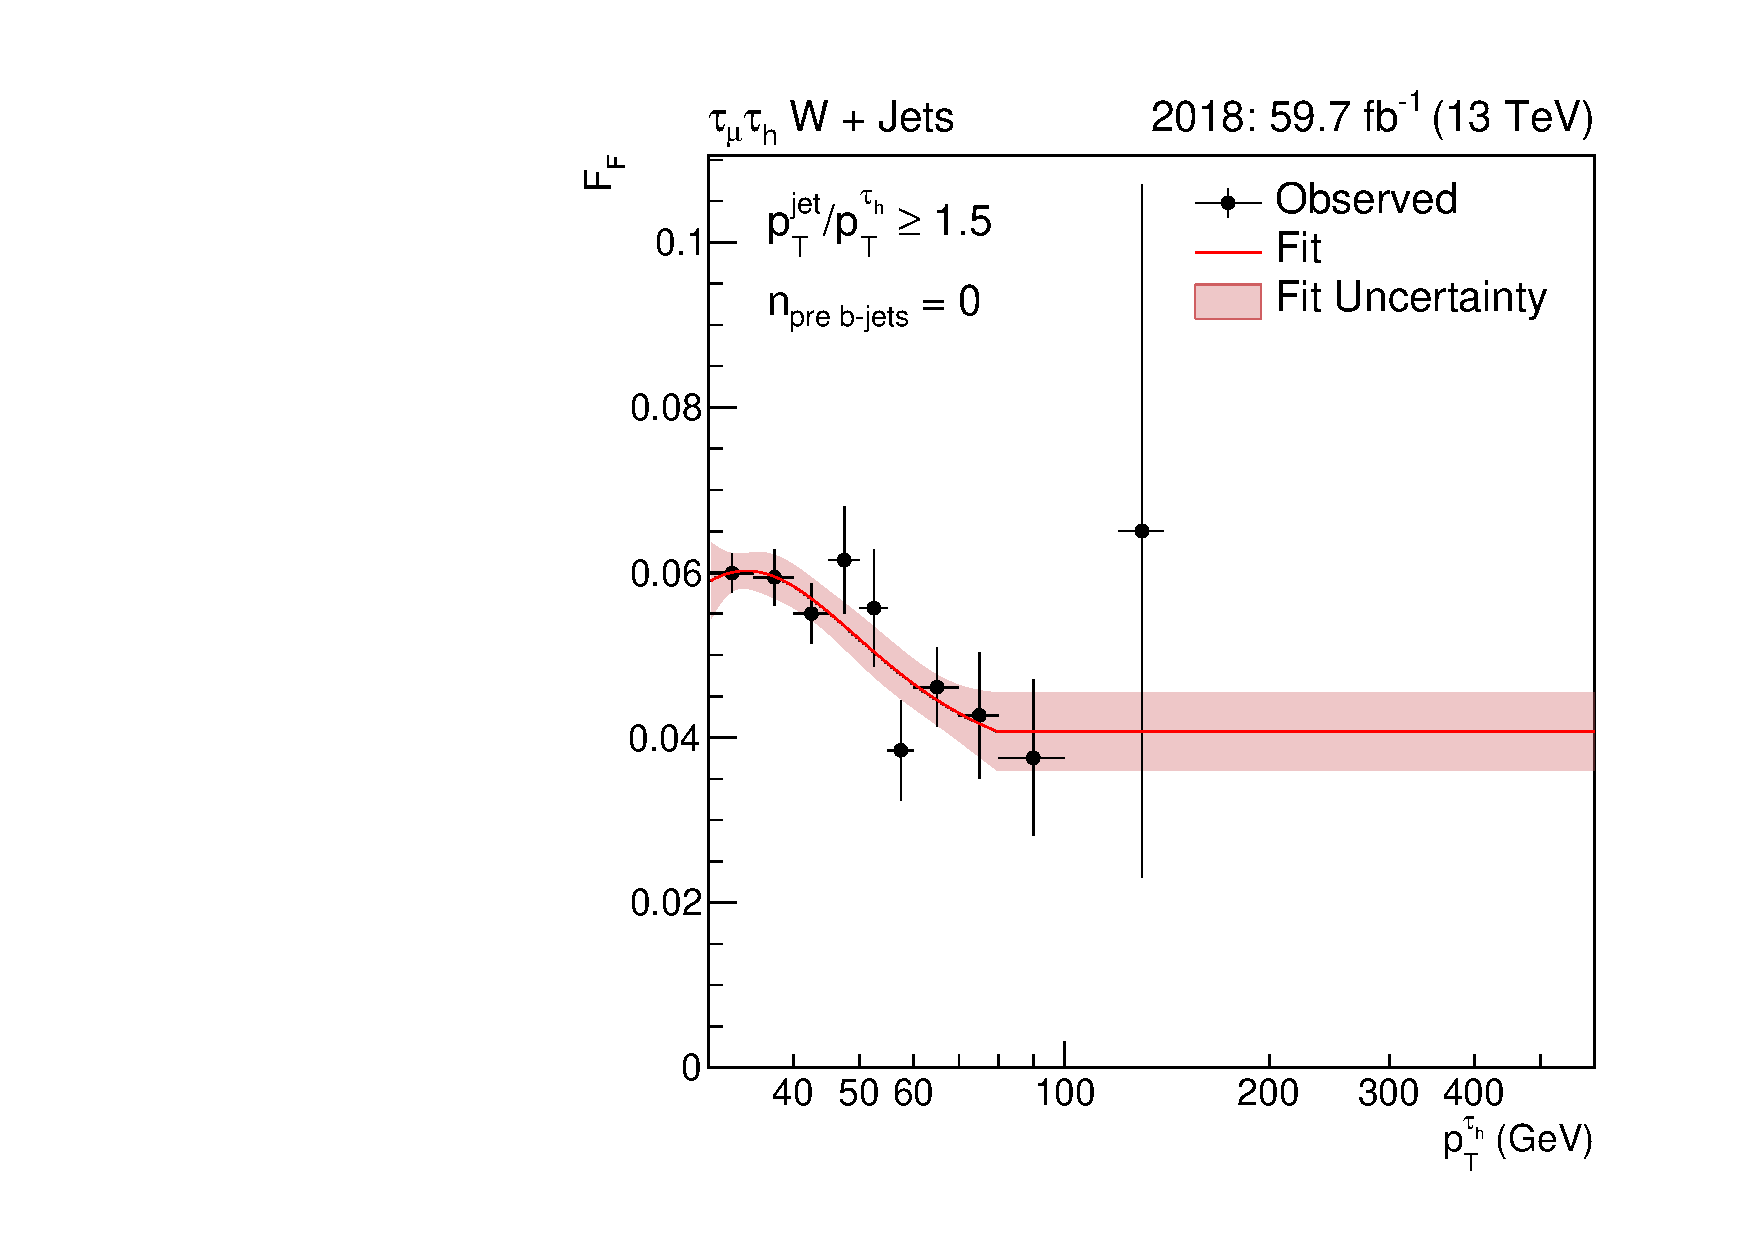
\includegraphics[width=0.33\textwidth]{Figures/ff_fit_jet_pt_high_0jet_pt_2_ff_wjets_mt_2018.pdf}} \\
\caption{Fake factor fits in $\mu\tauh$ channel for the QCD and W + Jets $n_{pre b jets}=0$ category with 2018 data. The three jet $\pT$ to hadronic tau $\pT$ categories are shown for each process.}
\label{fig:mt_ff_fit}
\end{figure}

\subsection{Corrections}

\begin{figure}[!hbtp]
\centering
    \subfloat[]{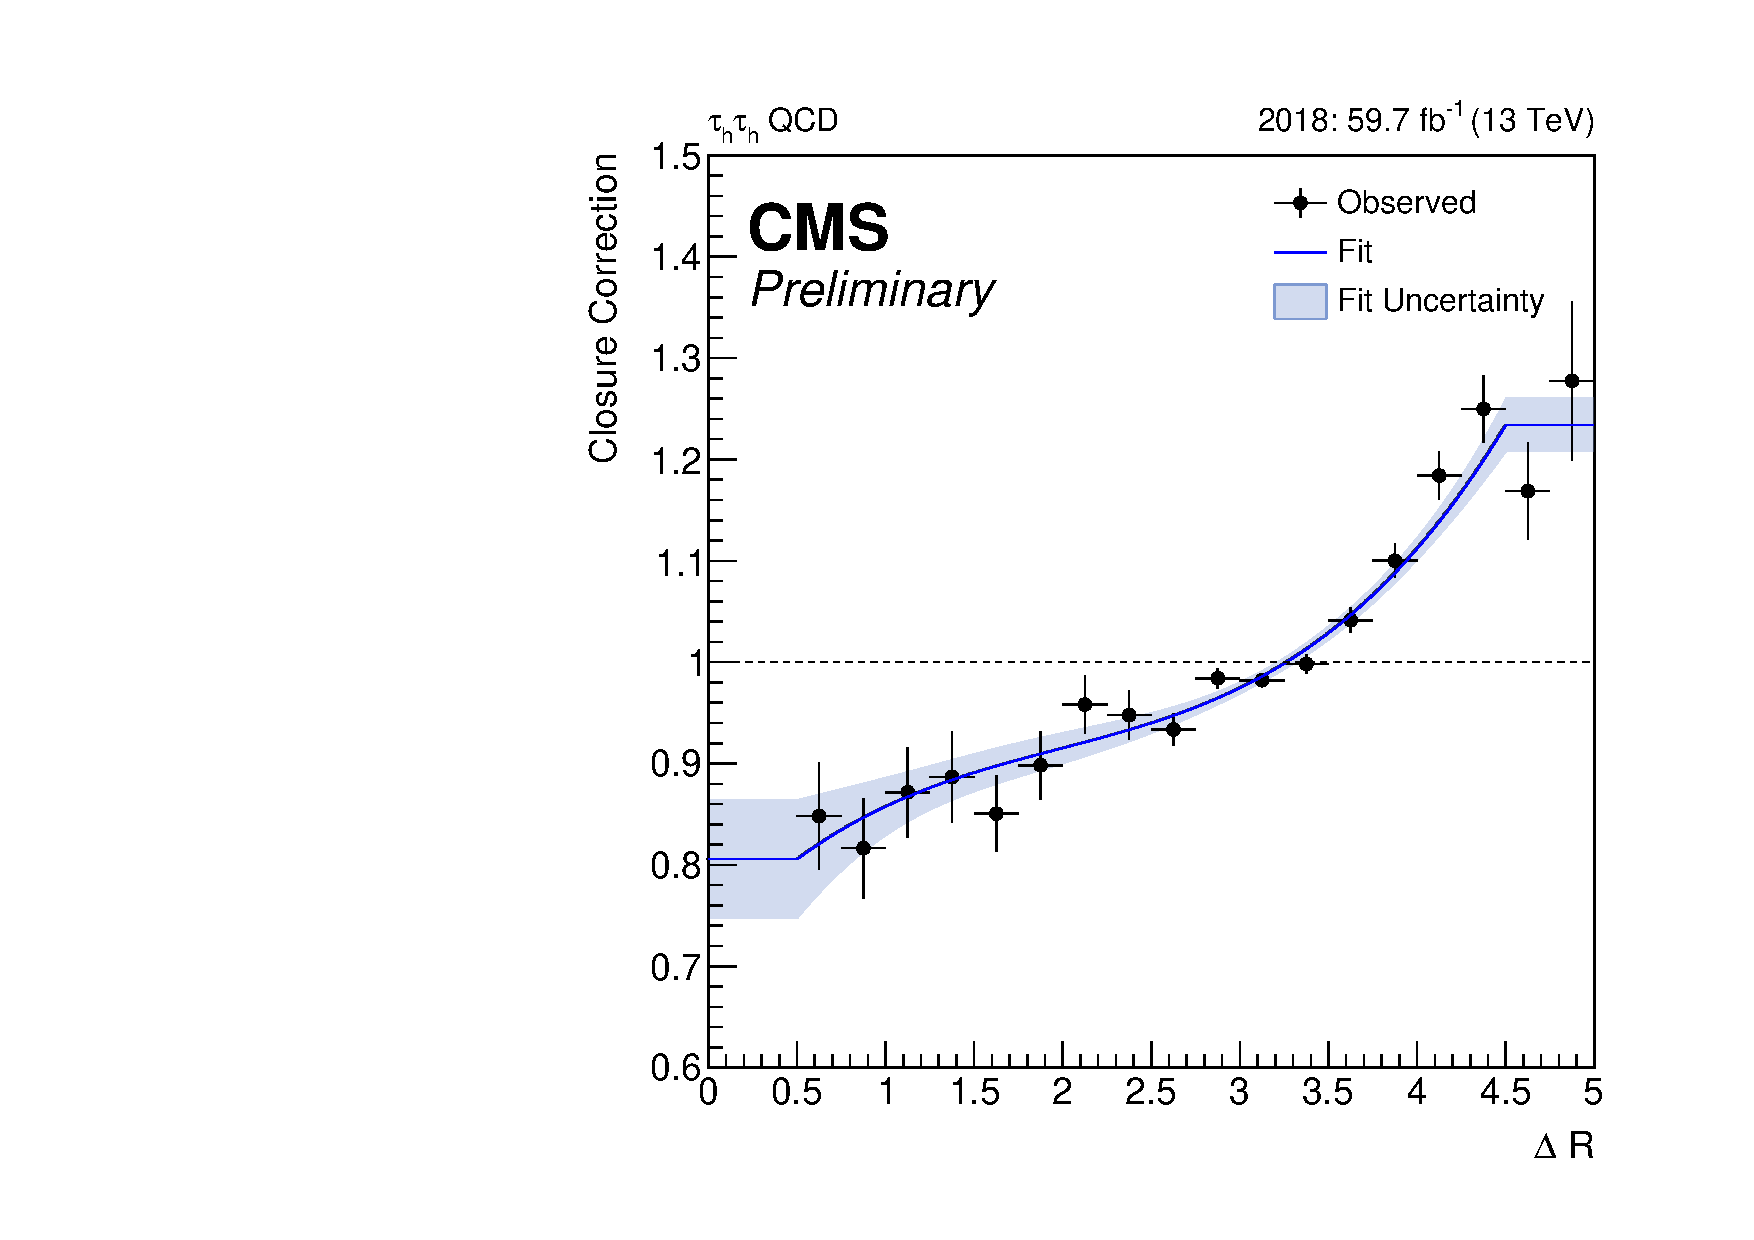
\includegraphics[width=0.33\textwidth]{Figures/ff_closure_ss_closure_nbjet0_qcd_tt_2018.pdf}} 
    \subfloat[]{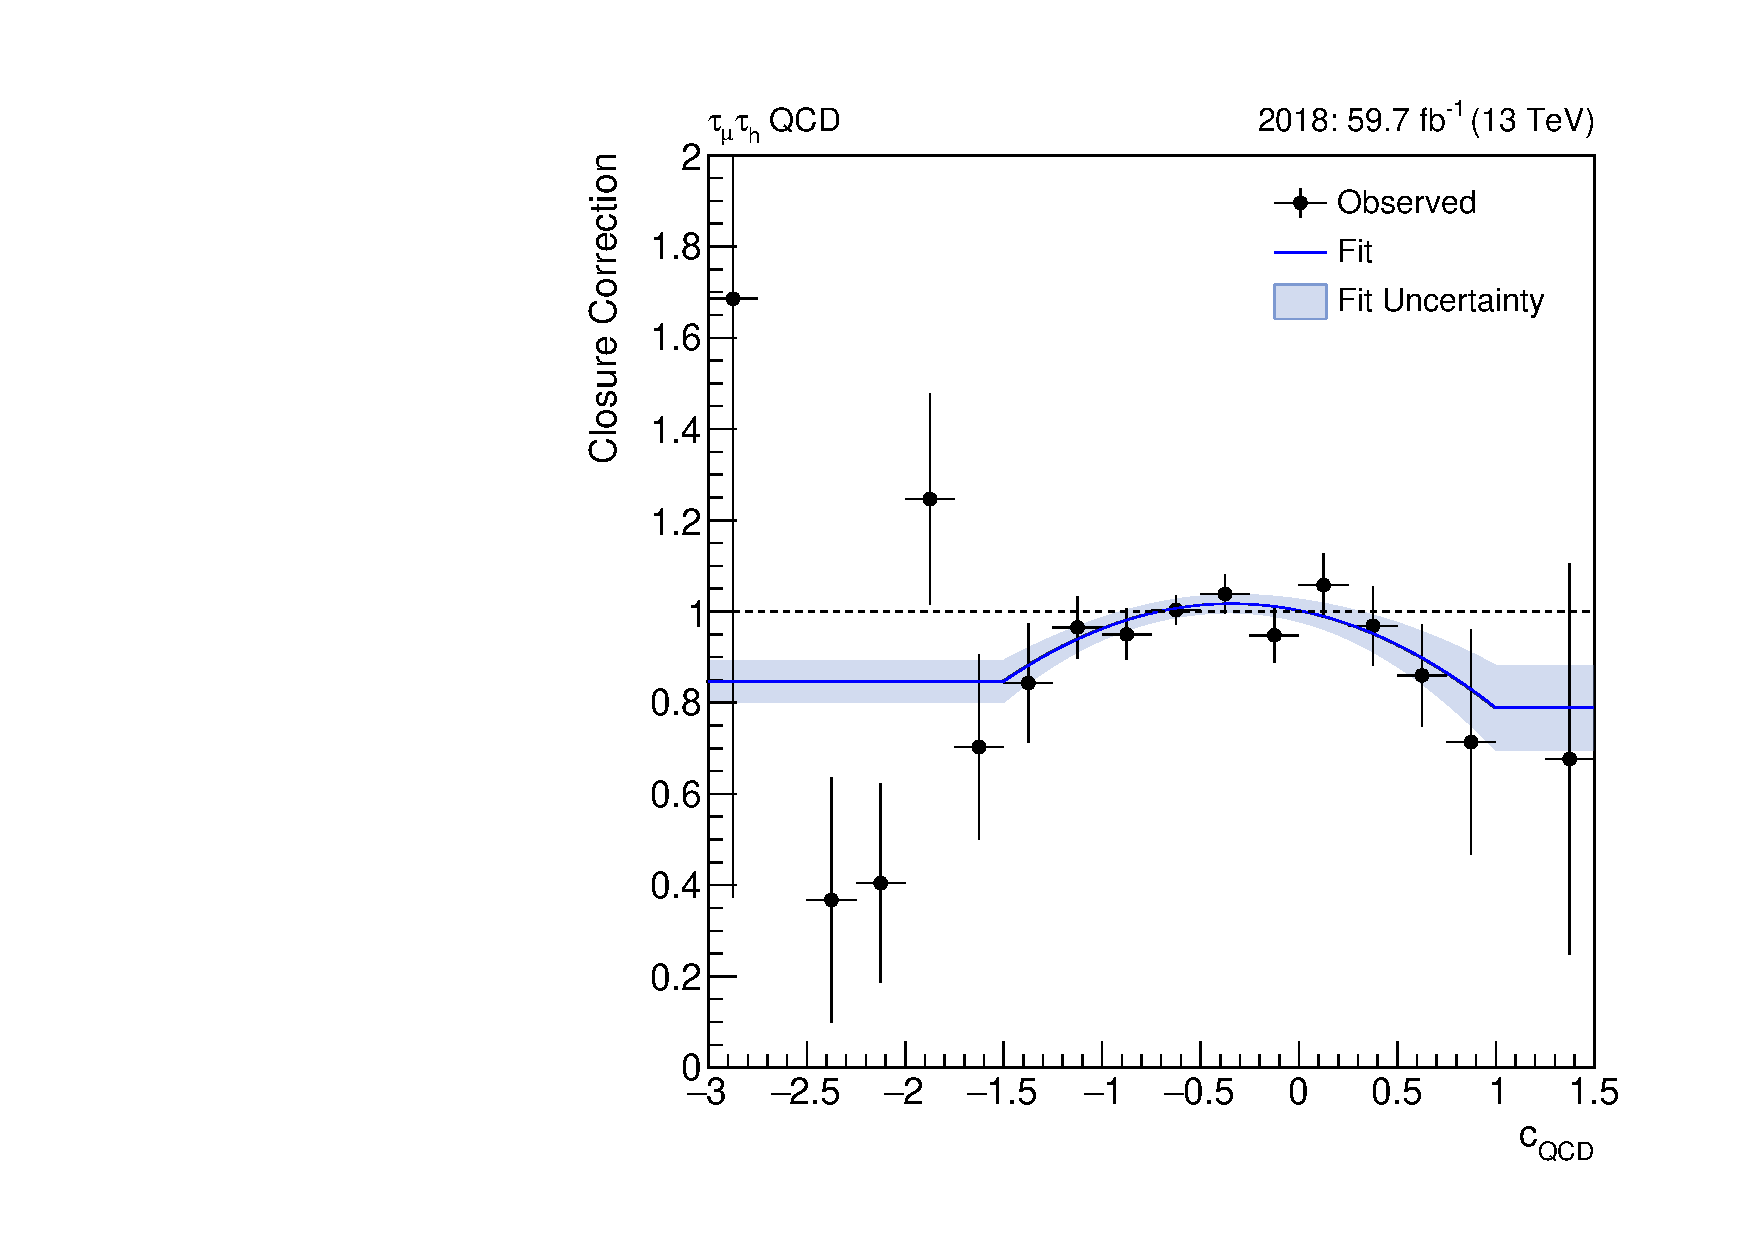
\includegraphics[width=0.33\textwidth]{Figures/ff_closure_met_0jet_closure_qcd_mt_2018.pdf}}
    \subfloat[]{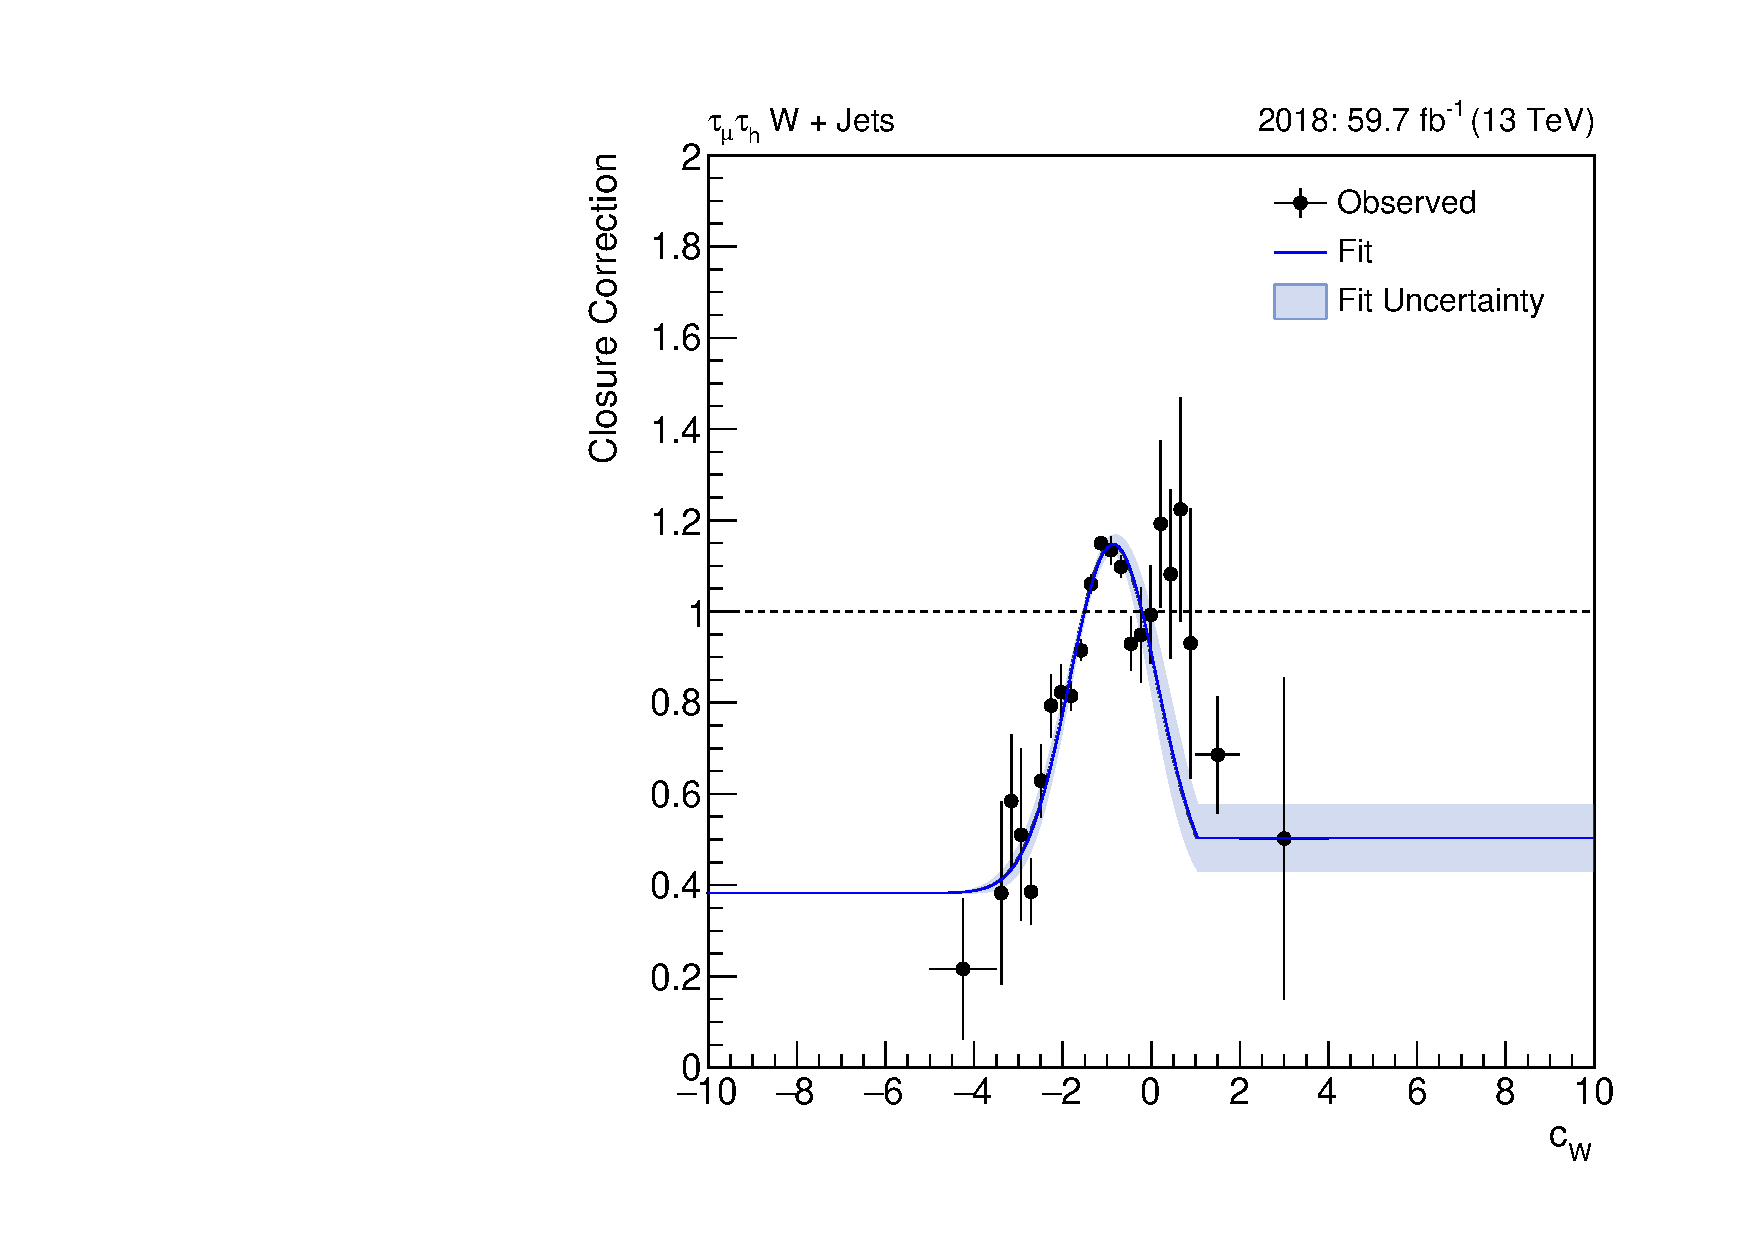
\includegraphics[width=0.33\textwidth]{Figures/ff_closure_met_0jet_closure_wjets_mt_2018.pdf}}
\caption{DR closures}
\label{fig:ff_dr}
\end{figure}

\begin{figure}[!hbtp]
\centering
    \subfloat[]{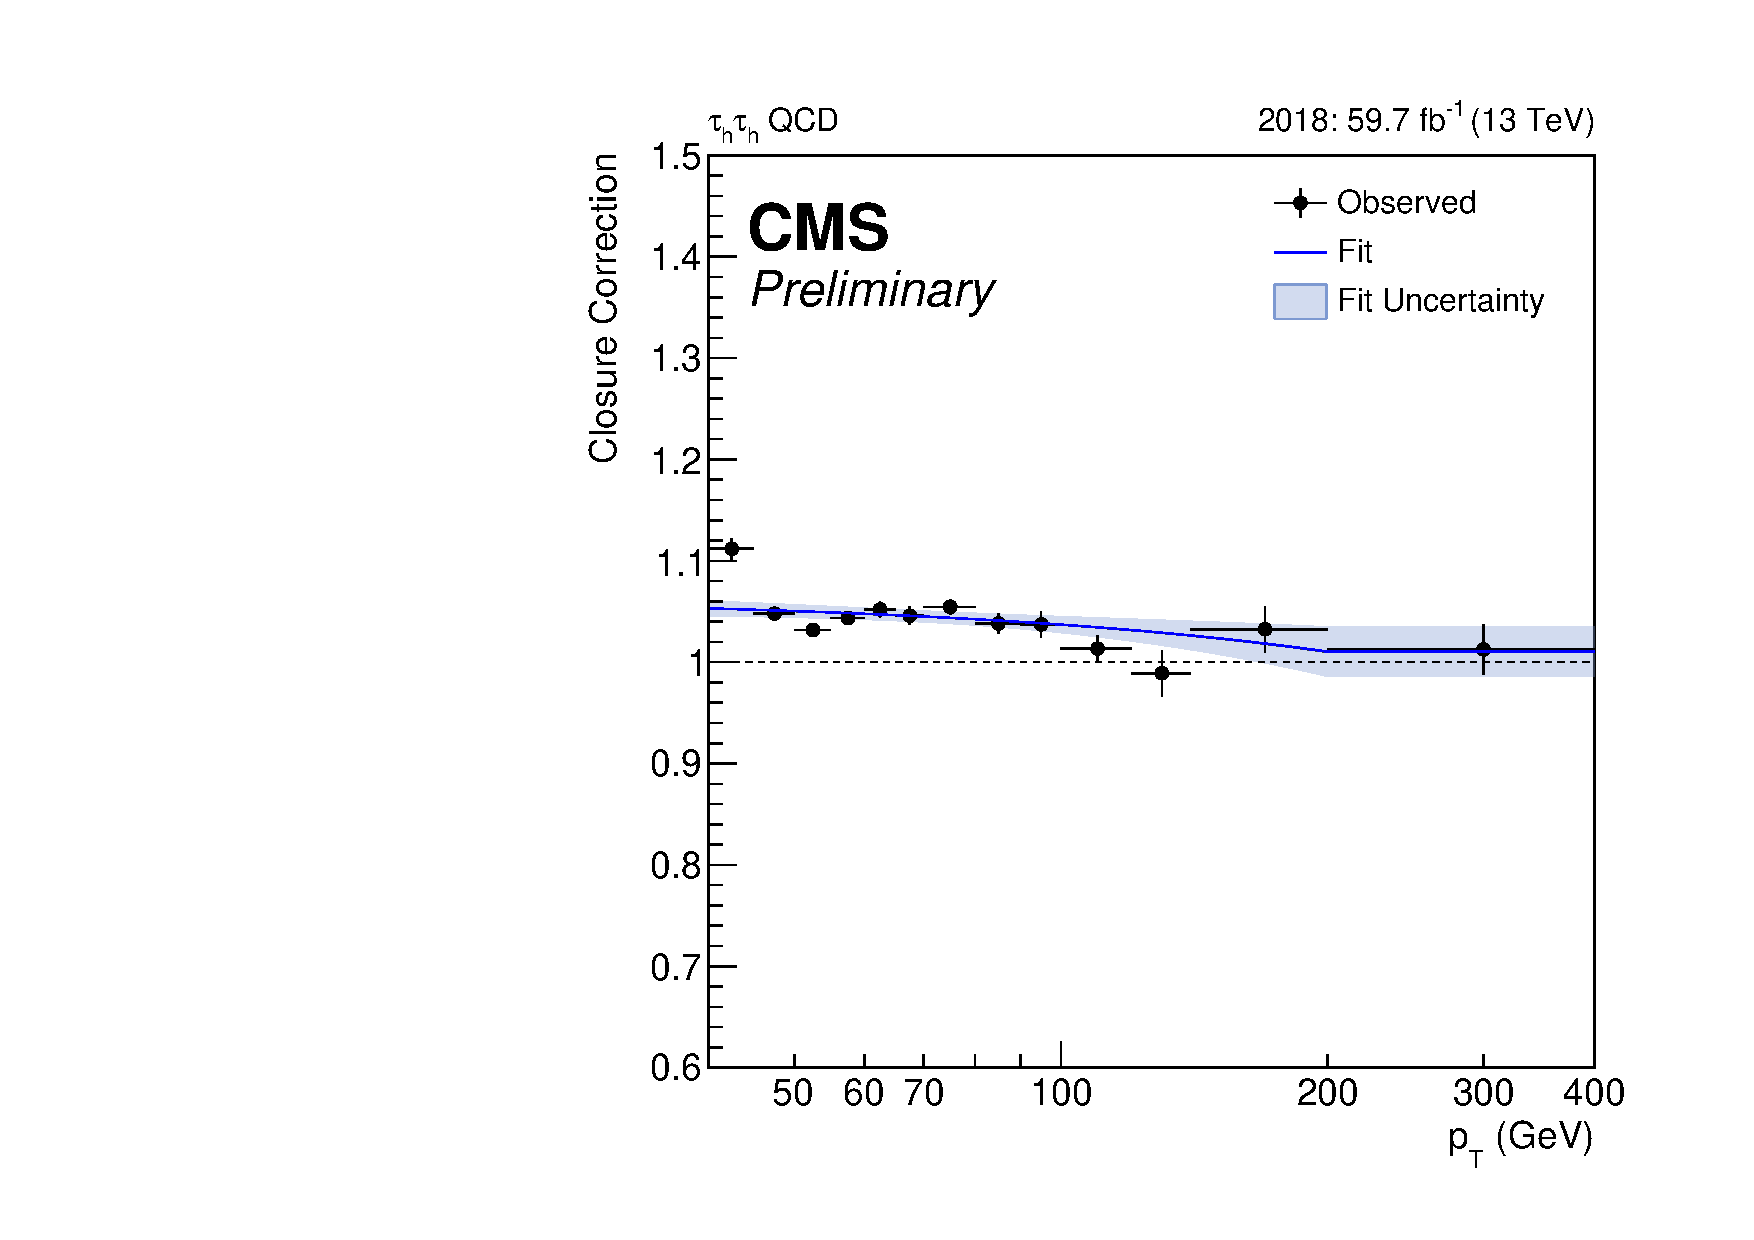
\includegraphics[width=0.33\textwidth]{Figures/ff_closure_os_closure_nbjet0_alt_qcd_tt_2018.pdf}} 
    \subfloat[]{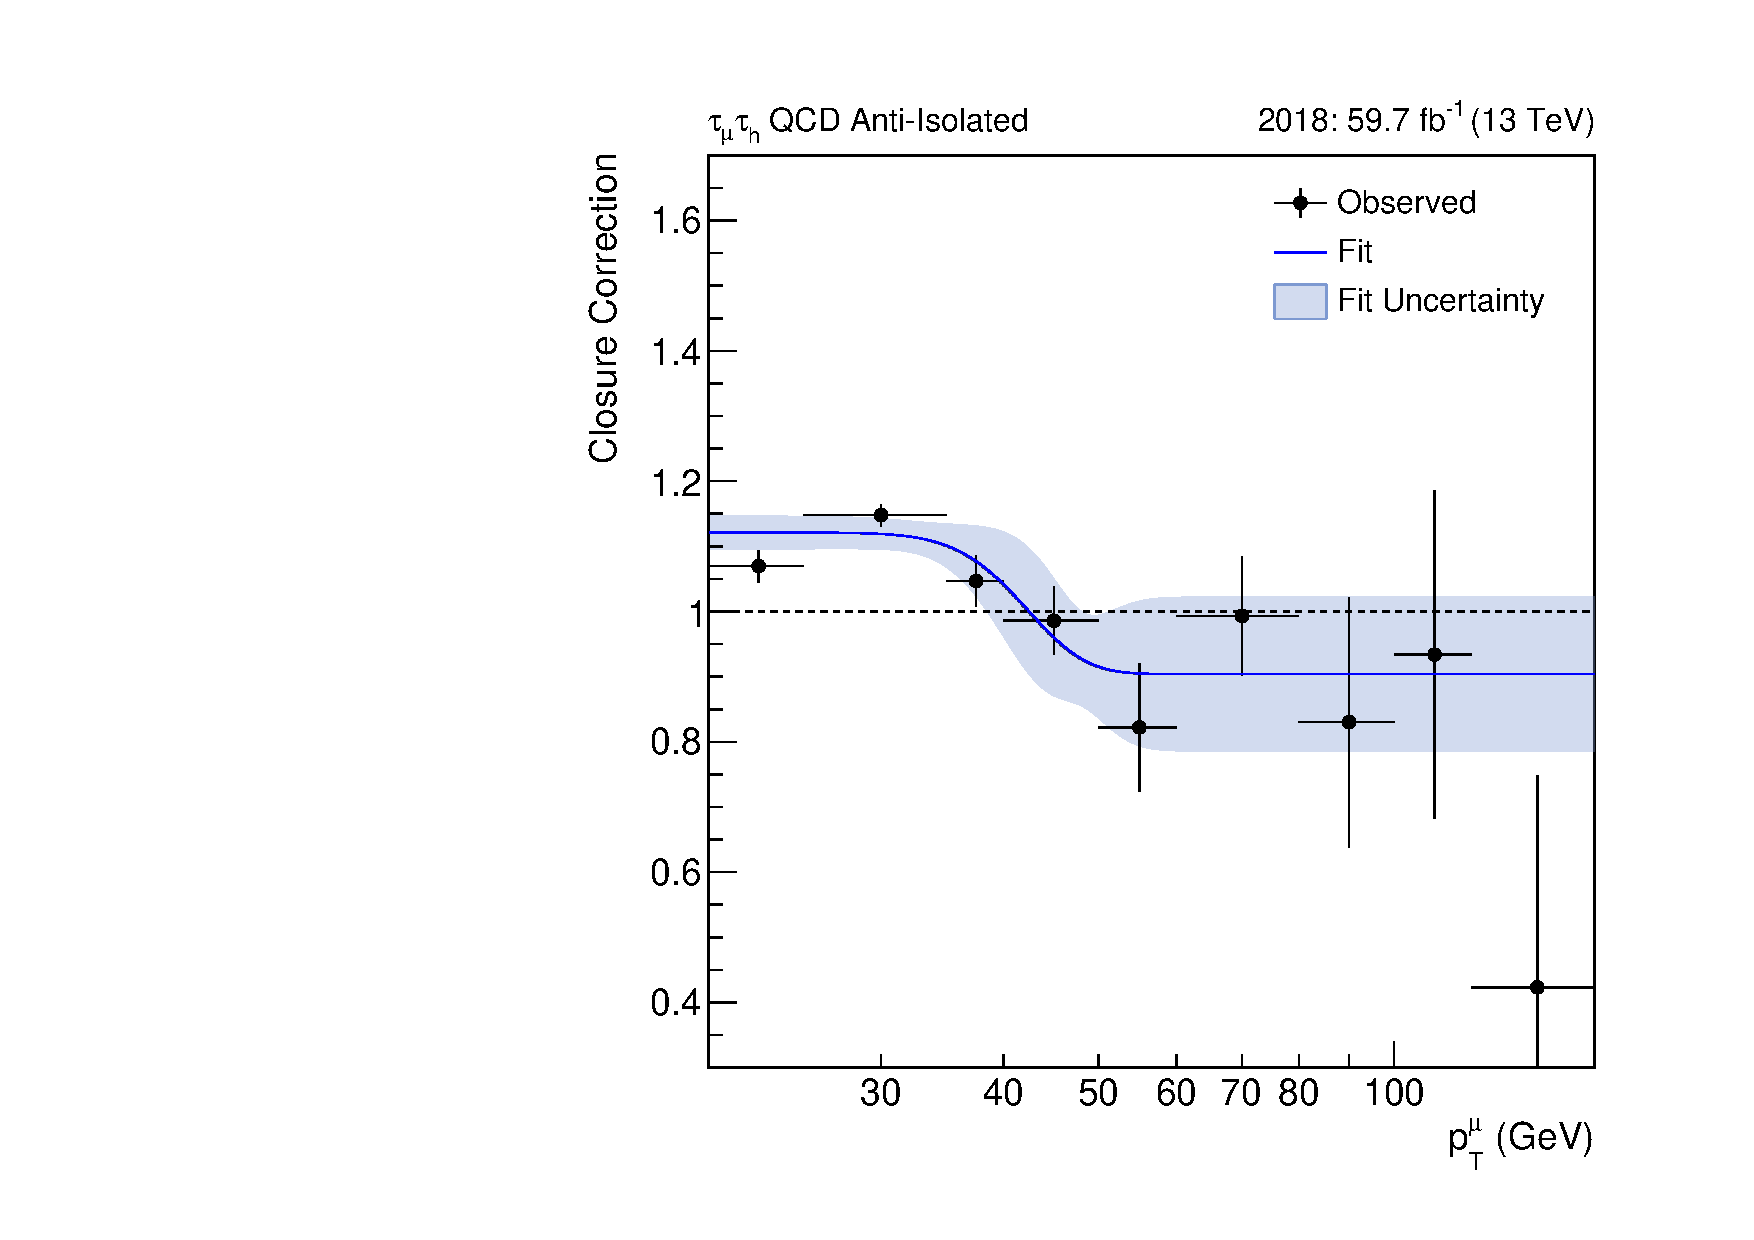
\includegraphics[width=0.33\textwidth]{Figures/ff_closure_pt_1_nbjets0_dr_to_ar_aiso_closure_qcd_mt_2018.pdf}}
    \subfloat[]{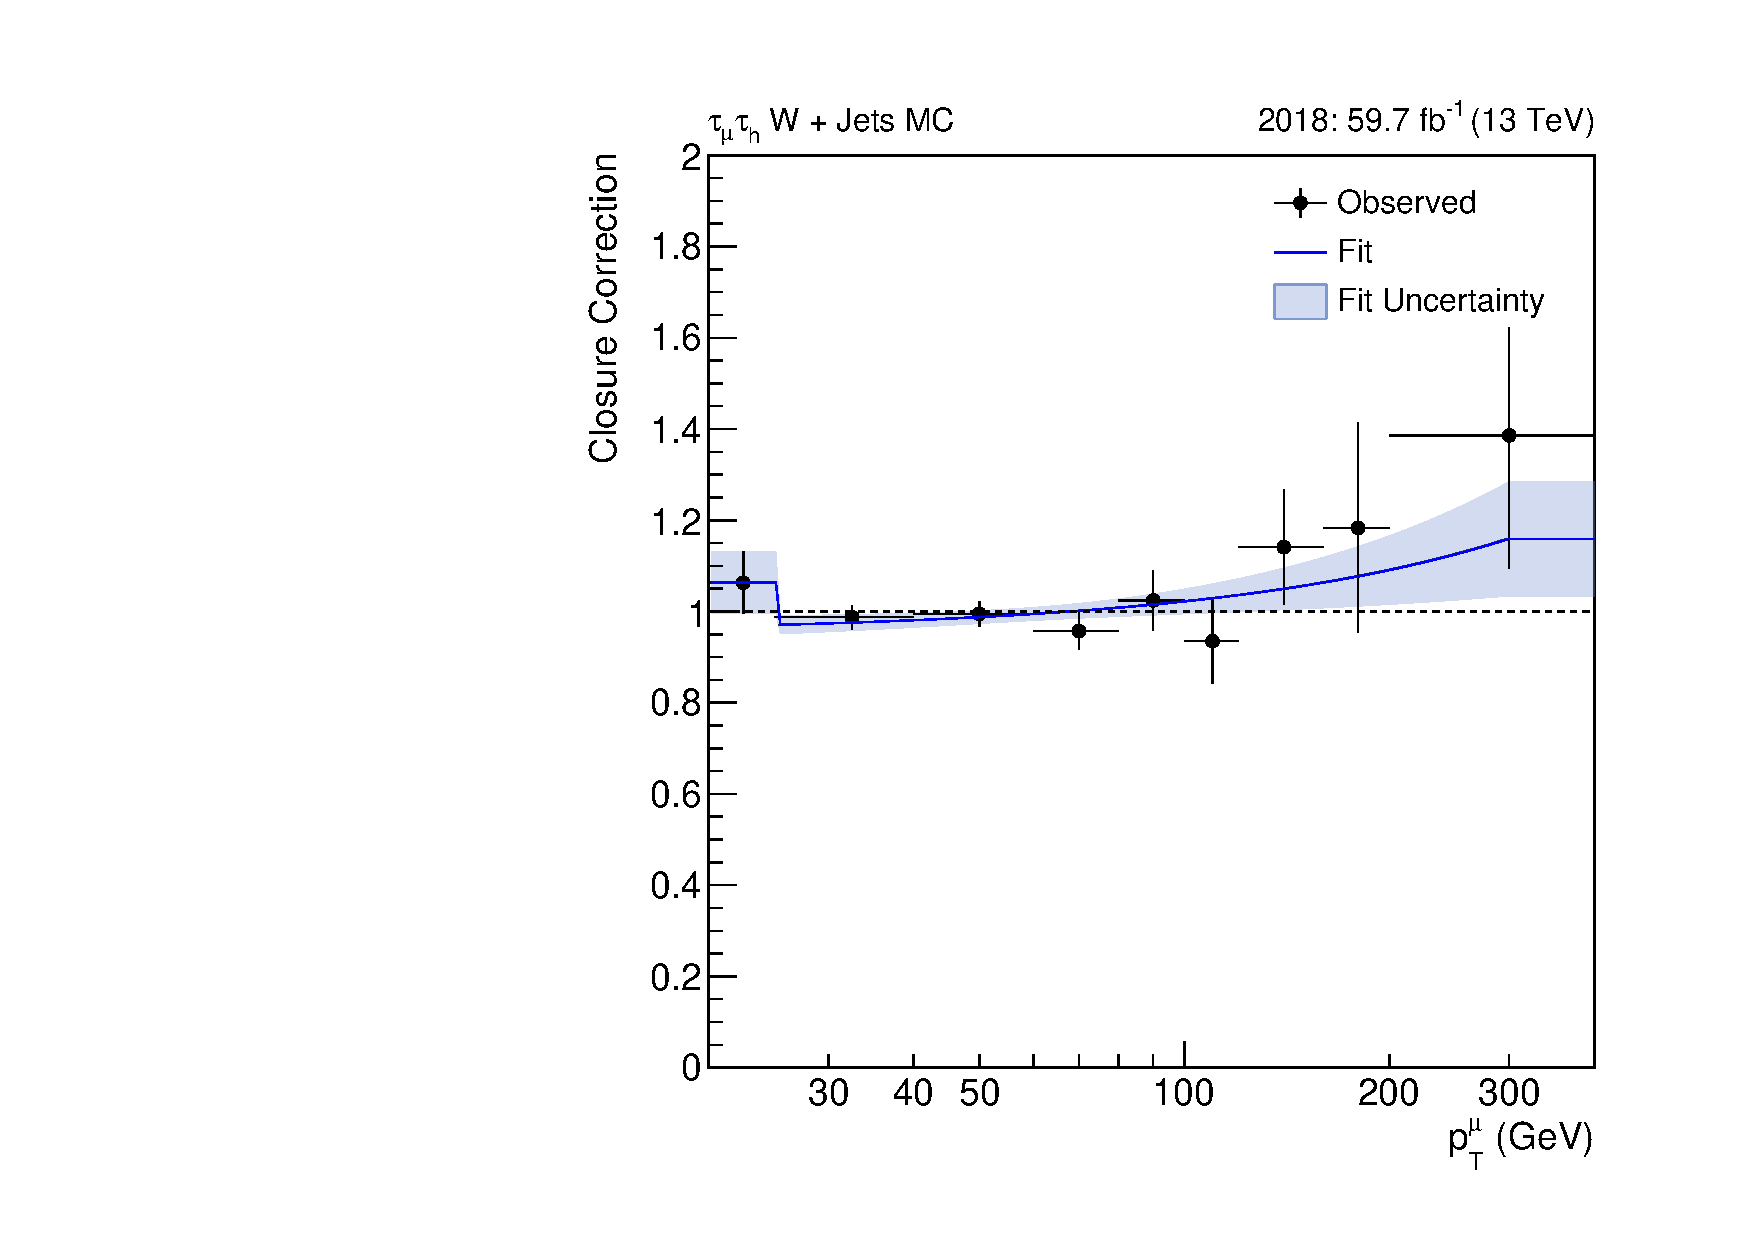
\includegraphics[width=0.33\textwidth]{Figures/ff_closure_pt_1_nbjets0_tightmt_dr_to_ar_closure_wjets_mc_mt_2018.pdf}}
\caption{DR to AR closures.}
\label{fig:ff_dr_to_ar}
\end{figure}


\subsection{Application Region Fractions}

\begin{figure}[!hbtp]
\centering
    \subfloat[]{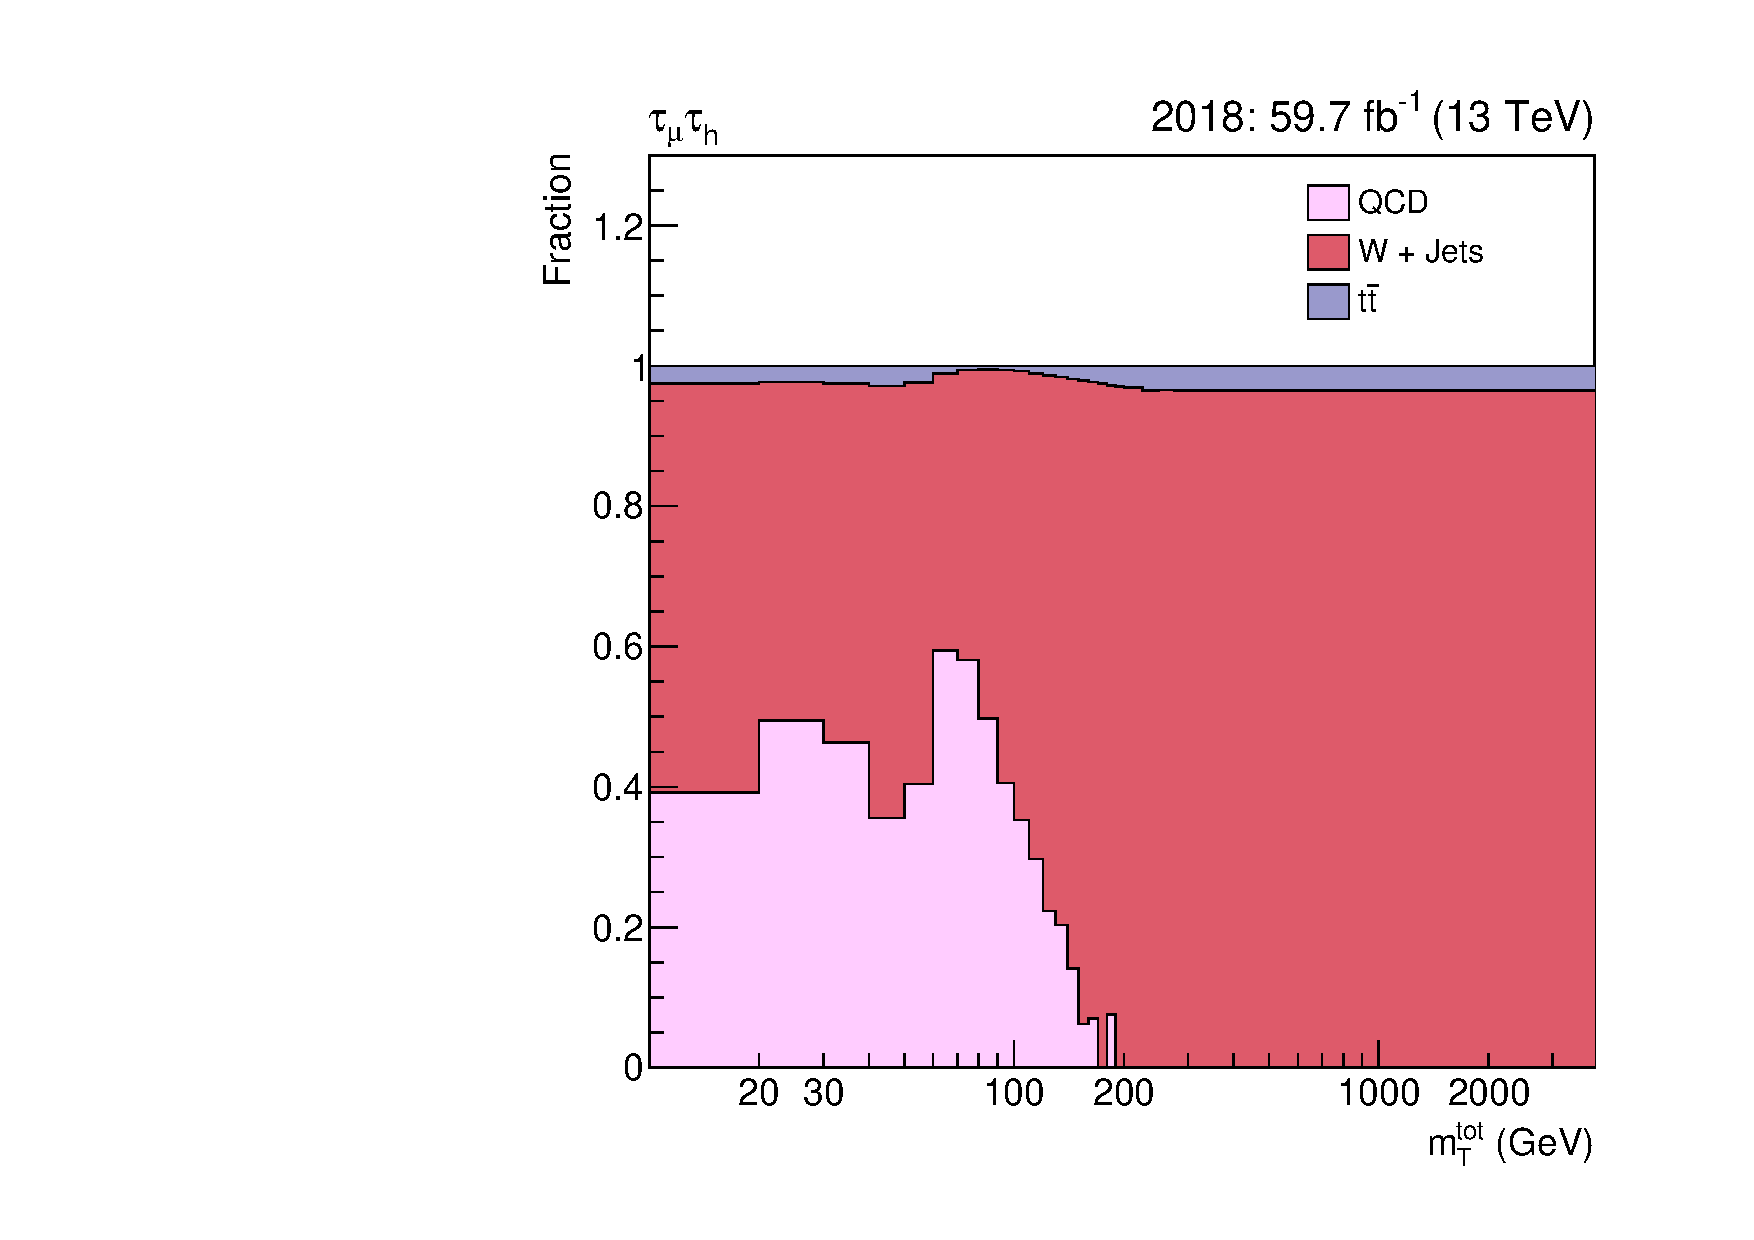
\includegraphics[width=0.45\textwidth]{Figures/ff_fraction_tightmt_nbjets0_mt_2018_os_rebinning.pdf}}
    \subfloat[]{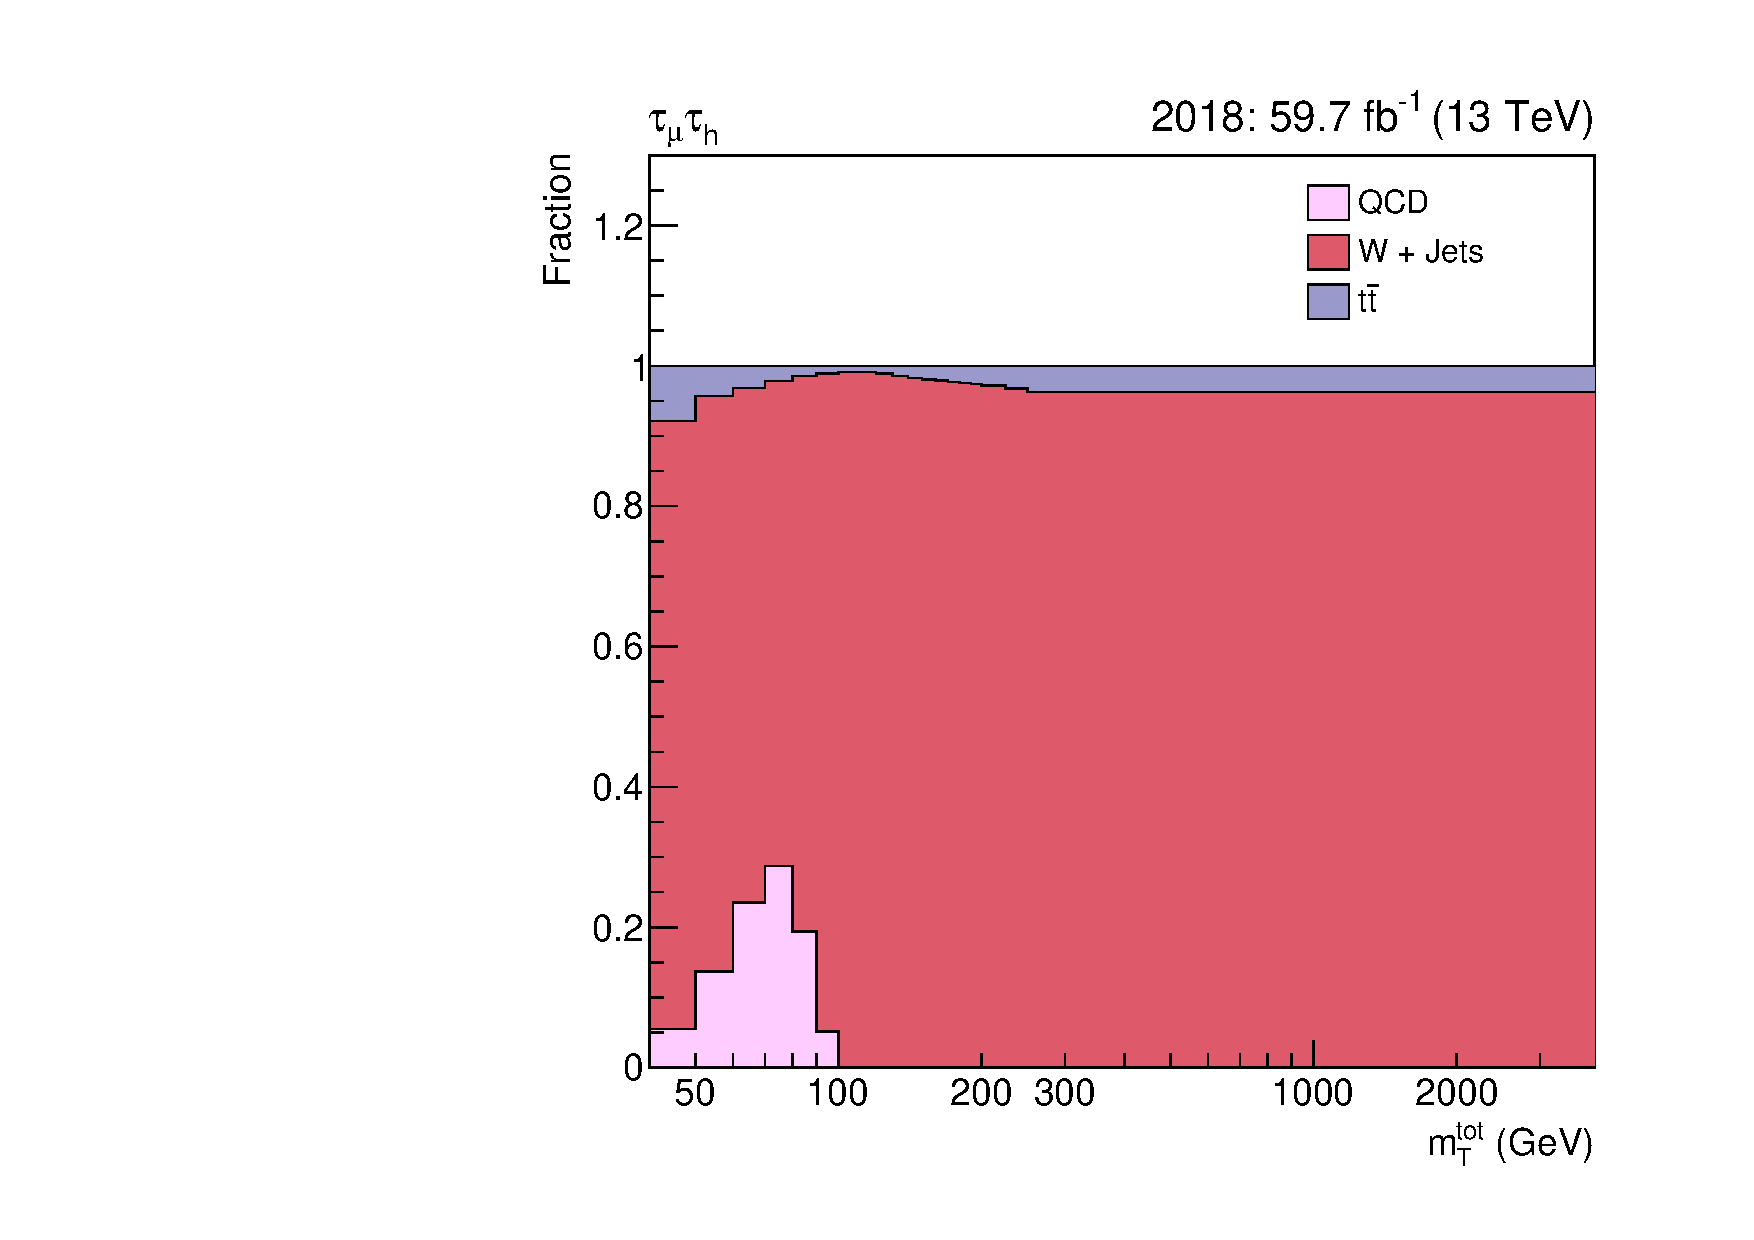
\includegraphics[width=0.45\textwidth]{Figures/ff_fraction_loosemt_nbjets0_mt_2018_os_rebinning.pdf}} \\
    \subfloat[]{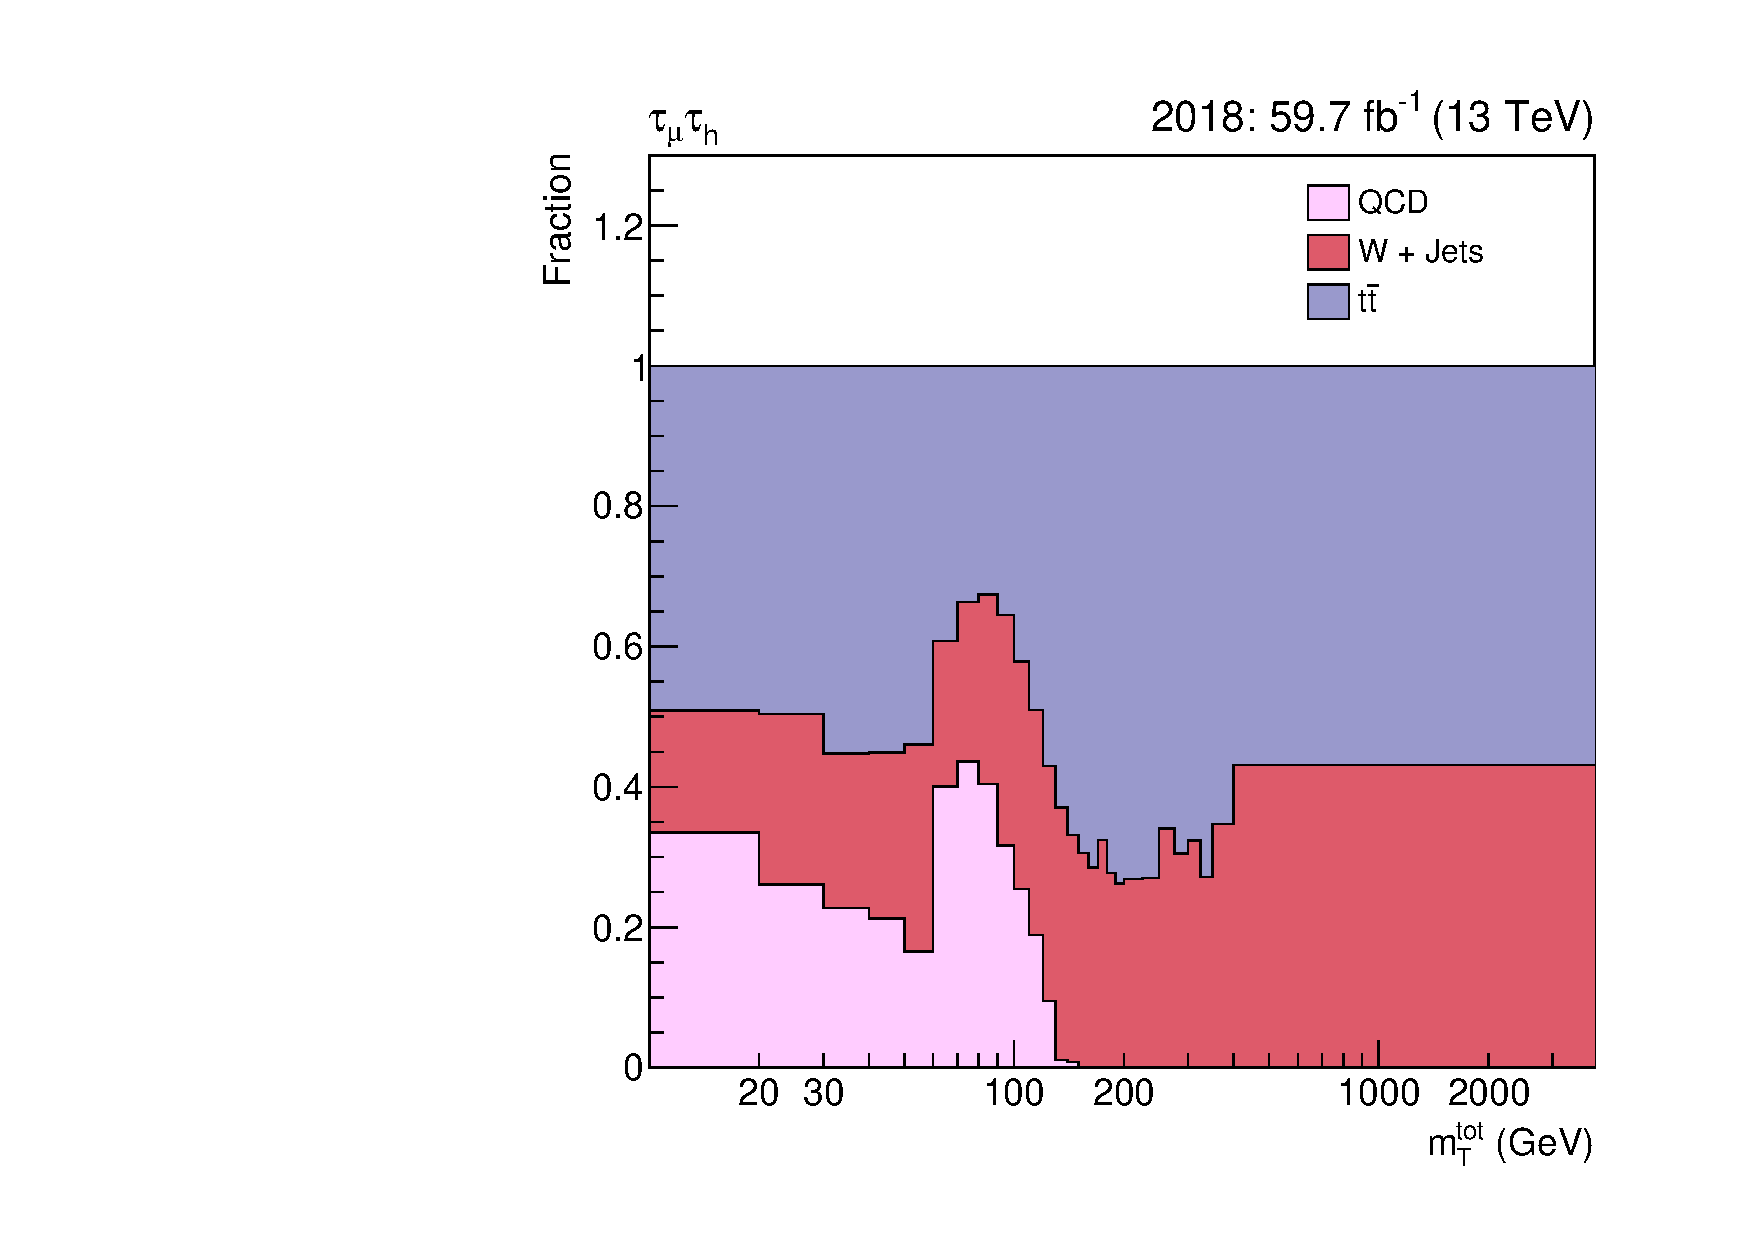
\includegraphics[width=0.45\textwidth]{Figures/ff_fraction_tightmt_nbjets1_mt_2018_os_rebinning.pdf}}
    \subfloat[]{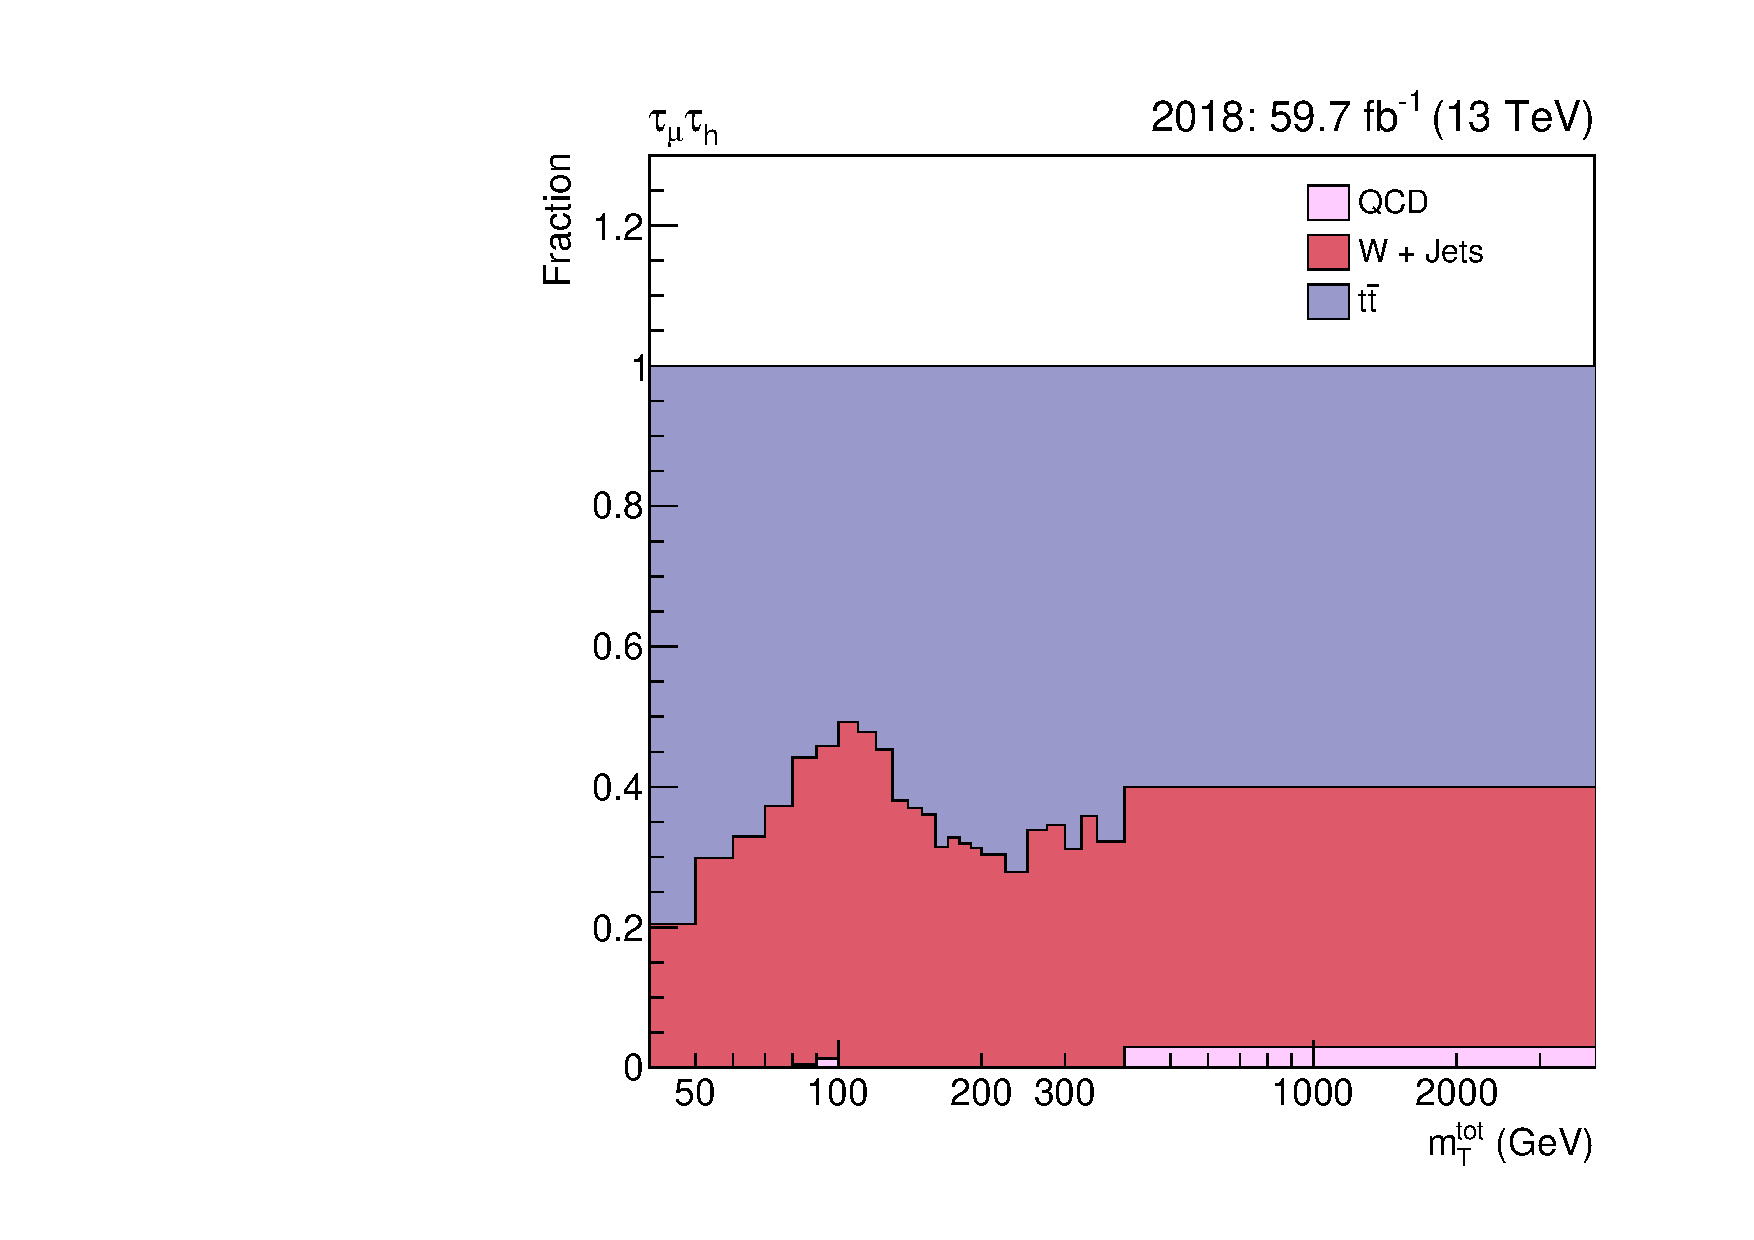
\includegraphics[width=0.45\textwidth]{Figures/ff_fraction_loosemt_nbjets1_mt_2018_os_rebinning.pdf}} \\
\caption{Fake factor fractions.}
\label{fig:mt_ff_frac}
\end{figure}


\subsection{Applying Fake Factors}
\label{sec:ff_applying}

using leading tau
subtracting off rest
w fakes in tt

\section{Uncertainty Model}

bulleted list of uncertainties used in the analysis.

\section{Postfit Plots}

\begin{figure}[!hbtp]
\centering
    \subfloat[]{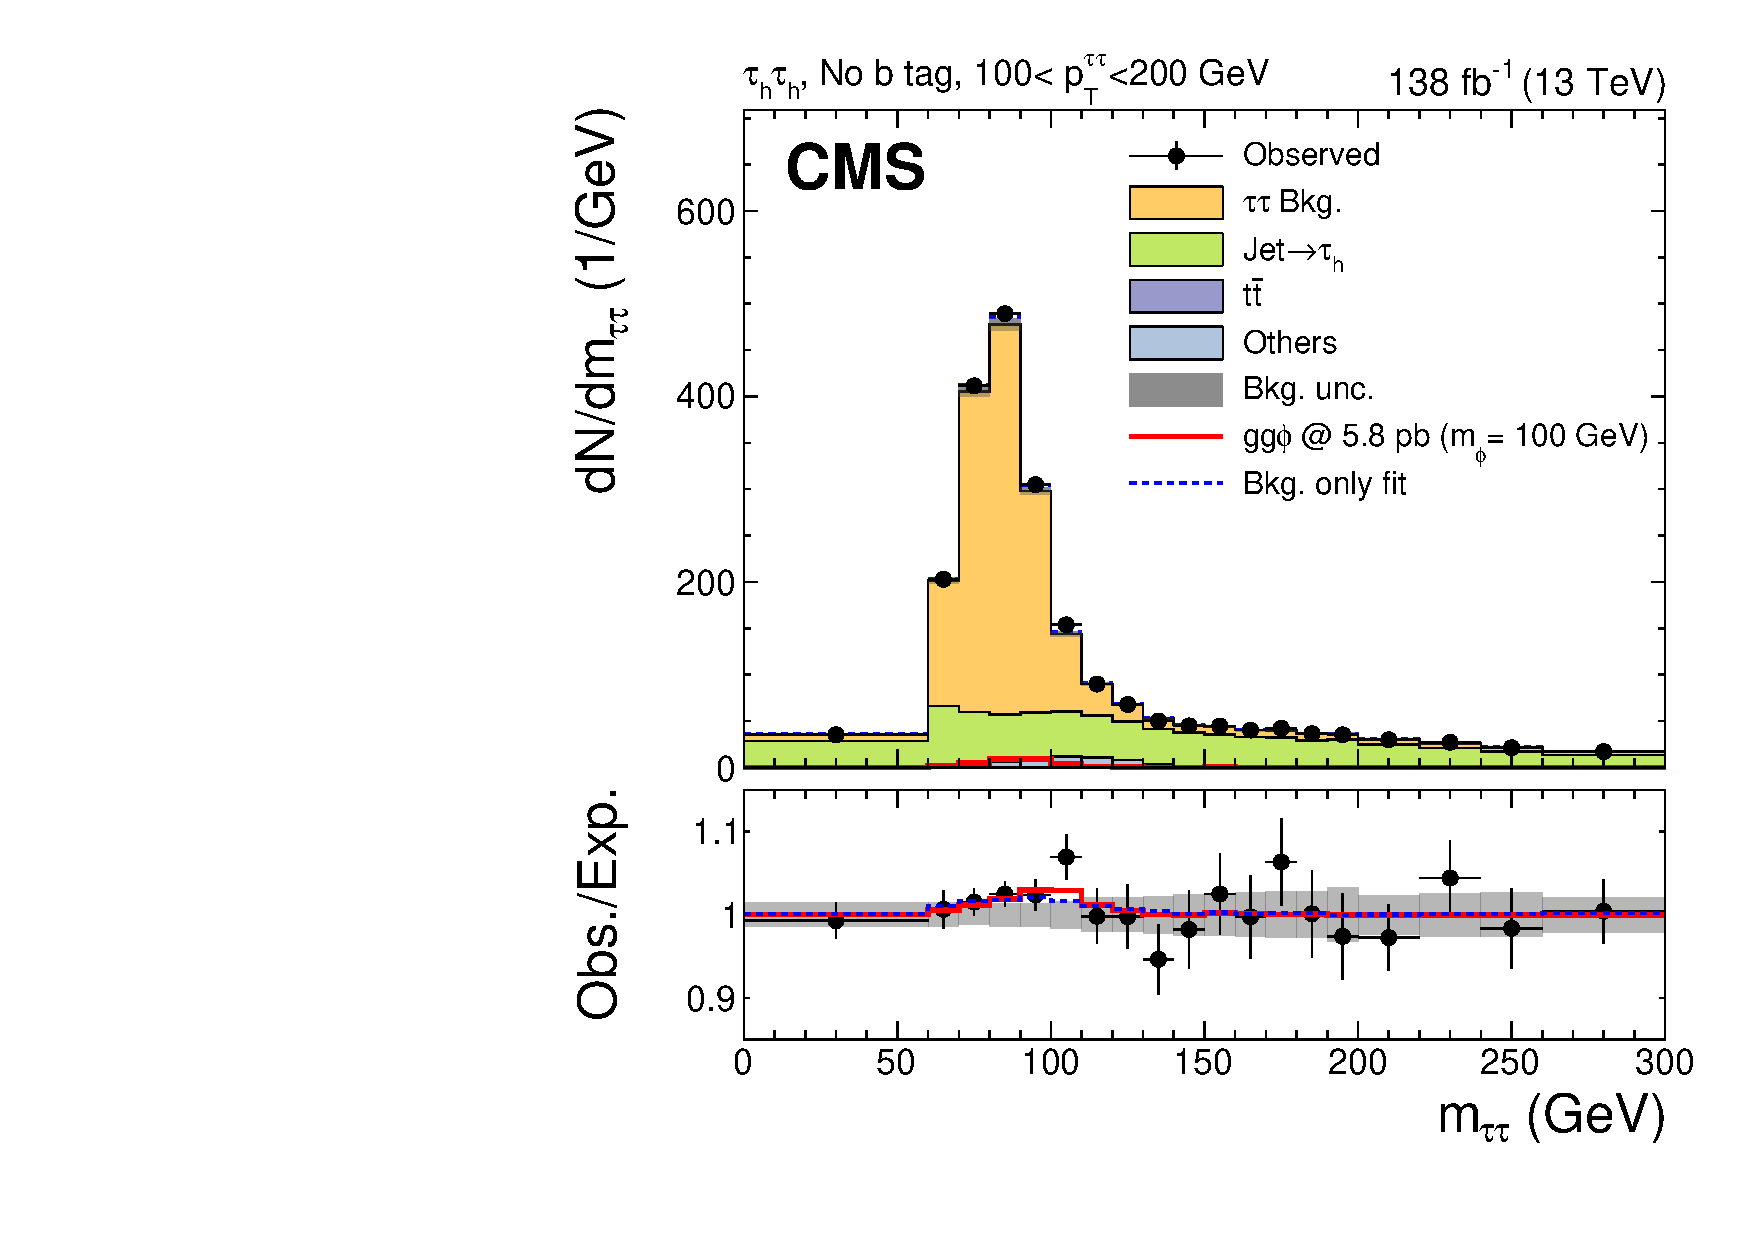
\includegraphics[width=0.45\textwidth]{Figures/postfit_lowmass_tt_nobtag_mediumpT.pdf}}
    \subfloat[]{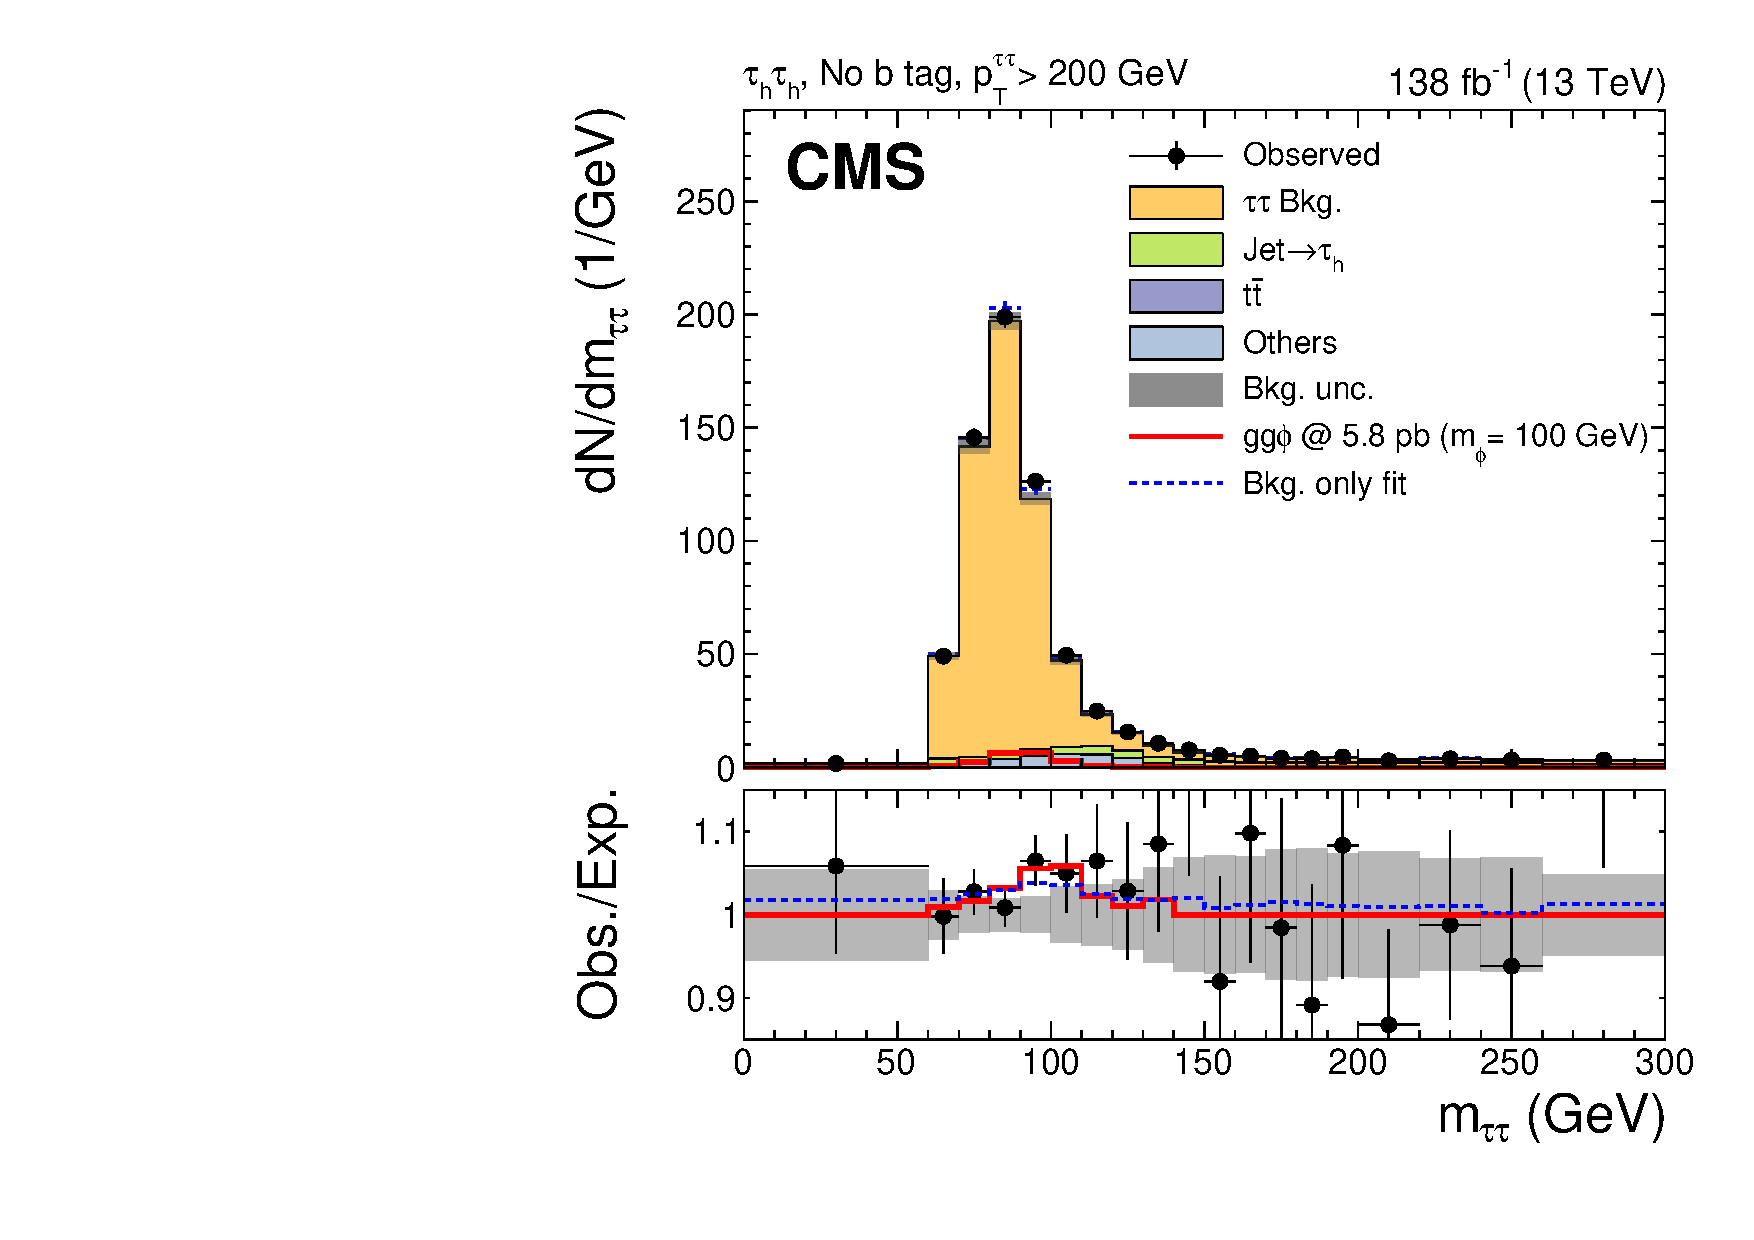
\includegraphics[width=0.45\textwidth]{Figures/postfit_lowmass_tt_nobtag_highpT.pdf}} \\
    \subfloat[]{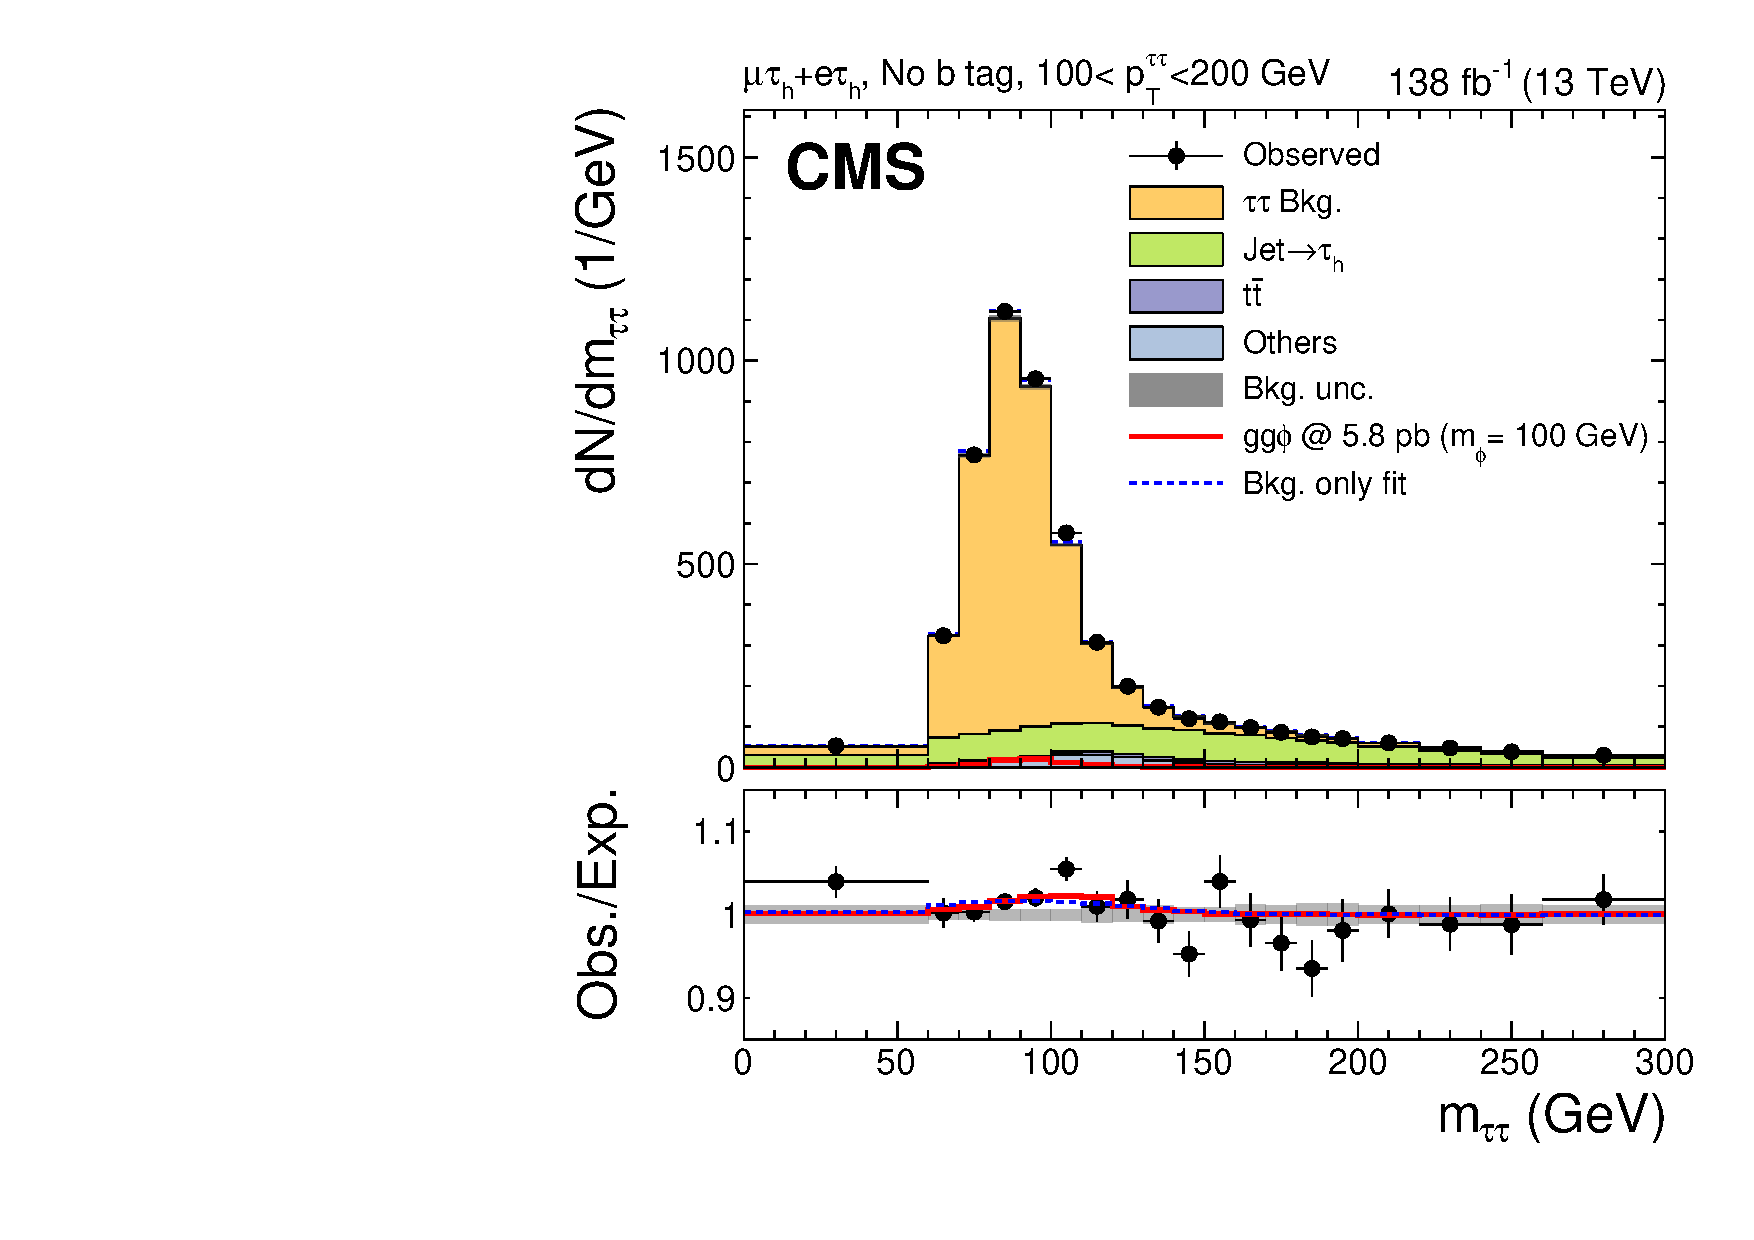
\includegraphics[width=0.45\textwidth]{Figures/postfit_lowmass_lt_nobtag_mediumpT.pdf}}
    \subfloat[]{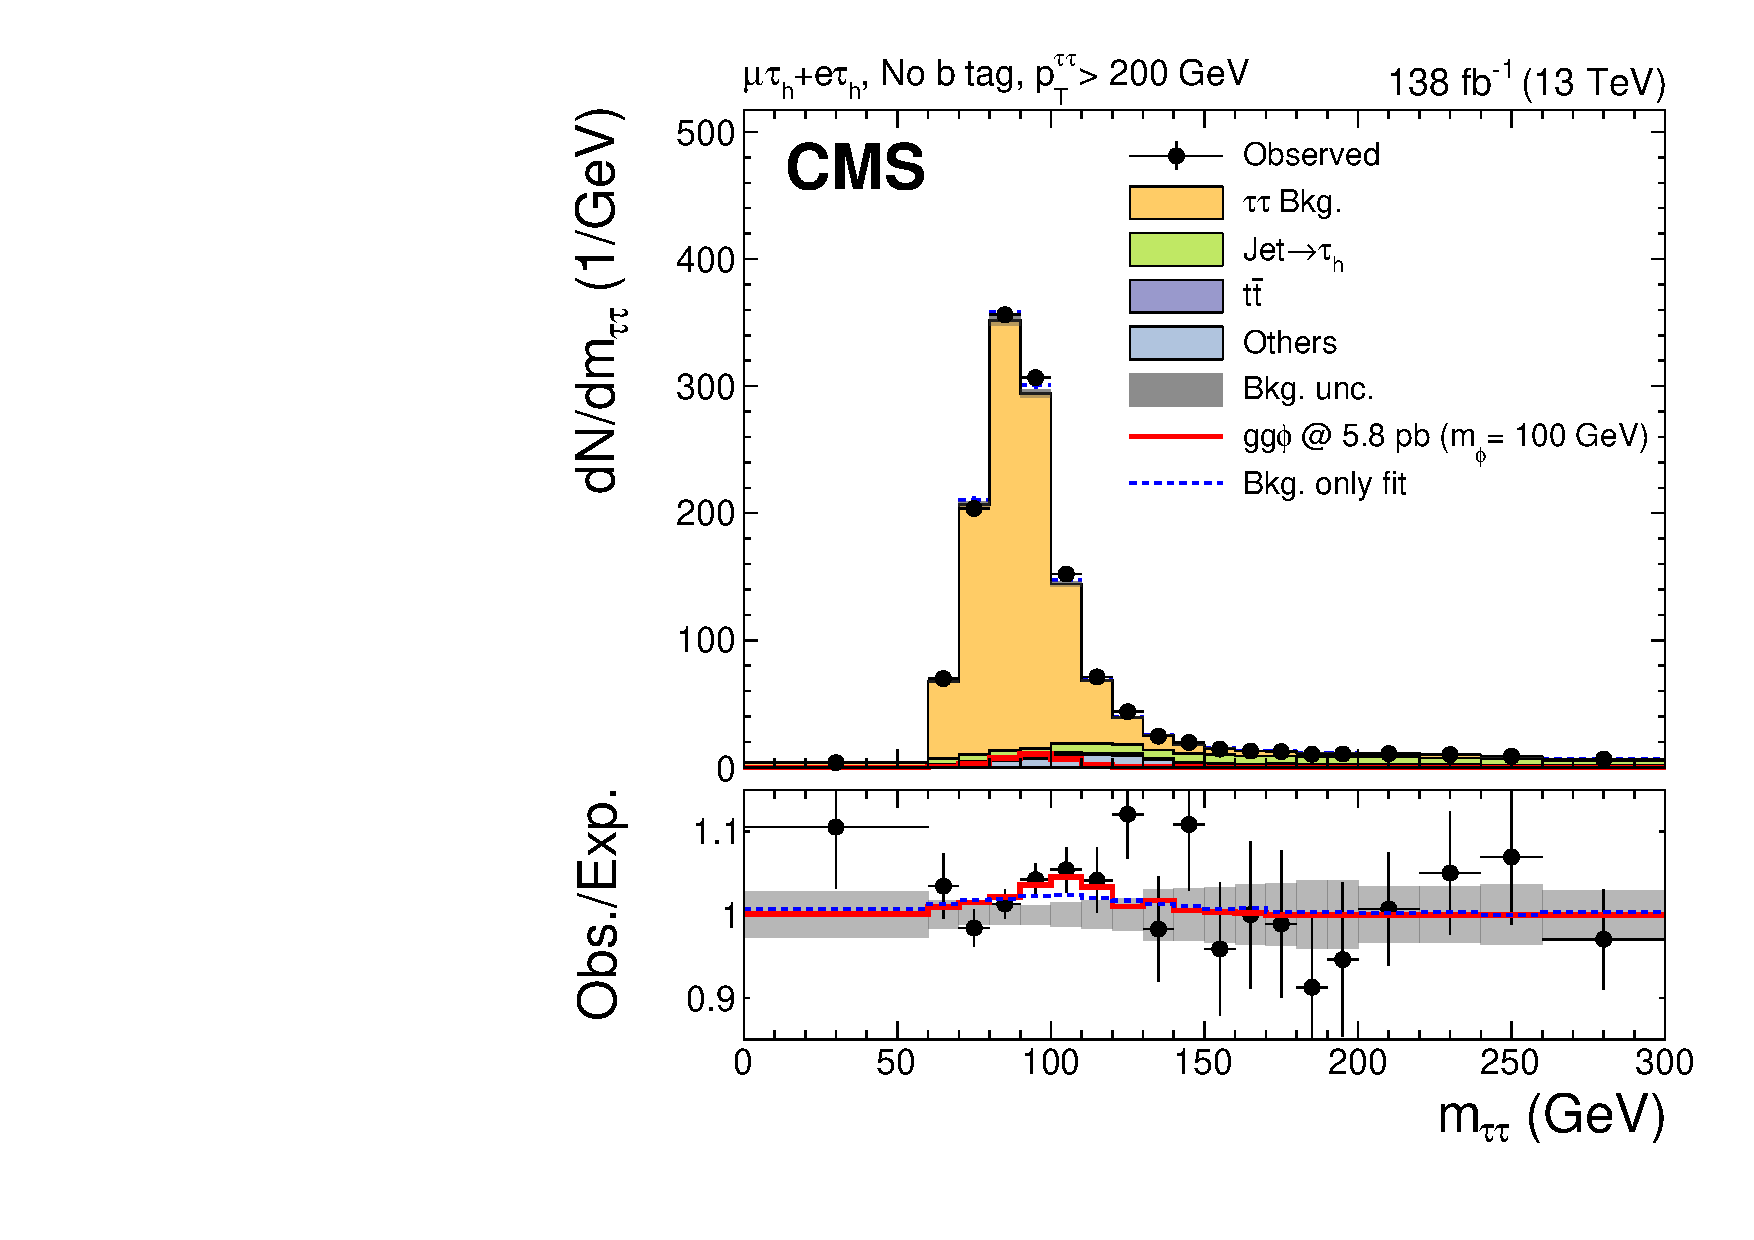
\includegraphics[width=0.45\textwidth]{Figures/postfit_lowmass_lt_nobtag_highpT.pdf}} \\
    \subfloat[]{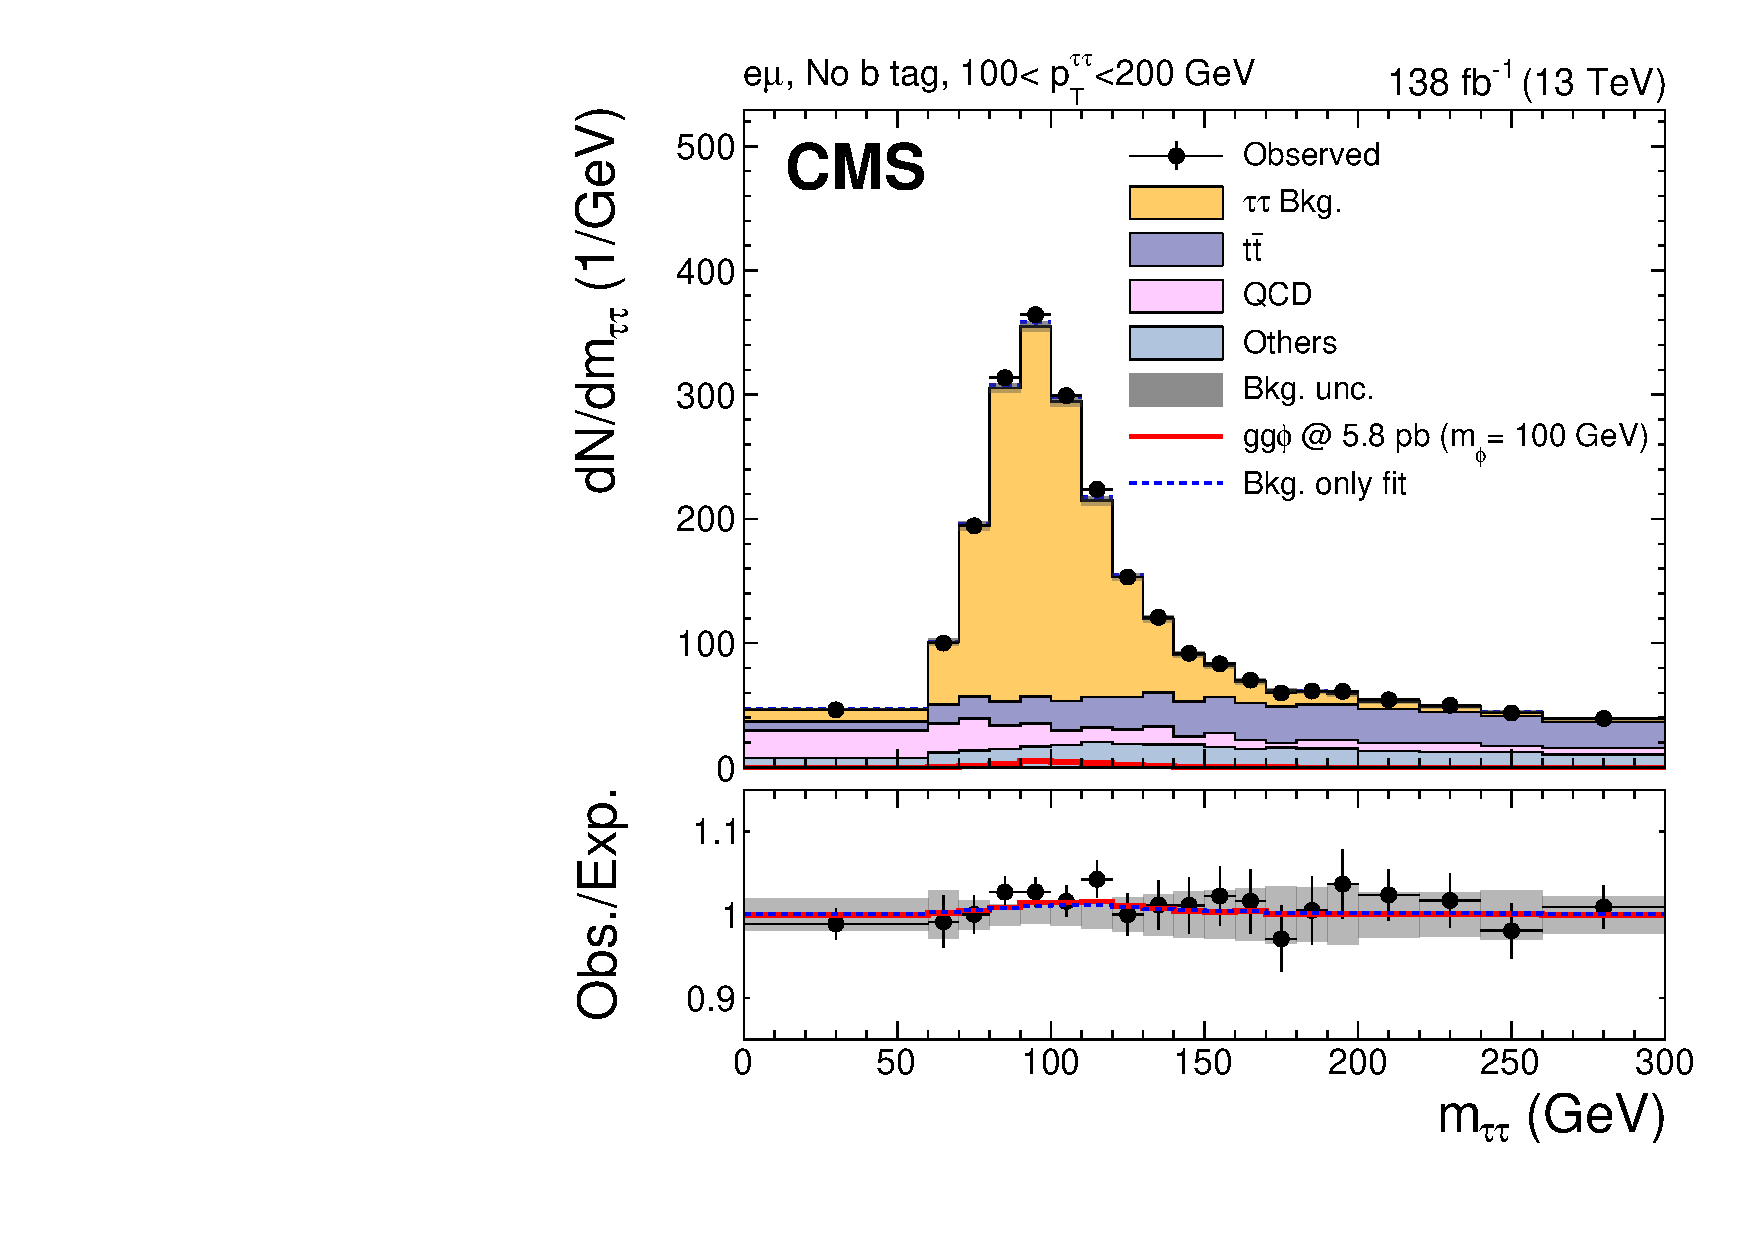
\includegraphics[width=0.45\textwidth]{Figures/postfit_lowmass_em_nobtag_mediumpT.pdf}}
    \subfloat[]{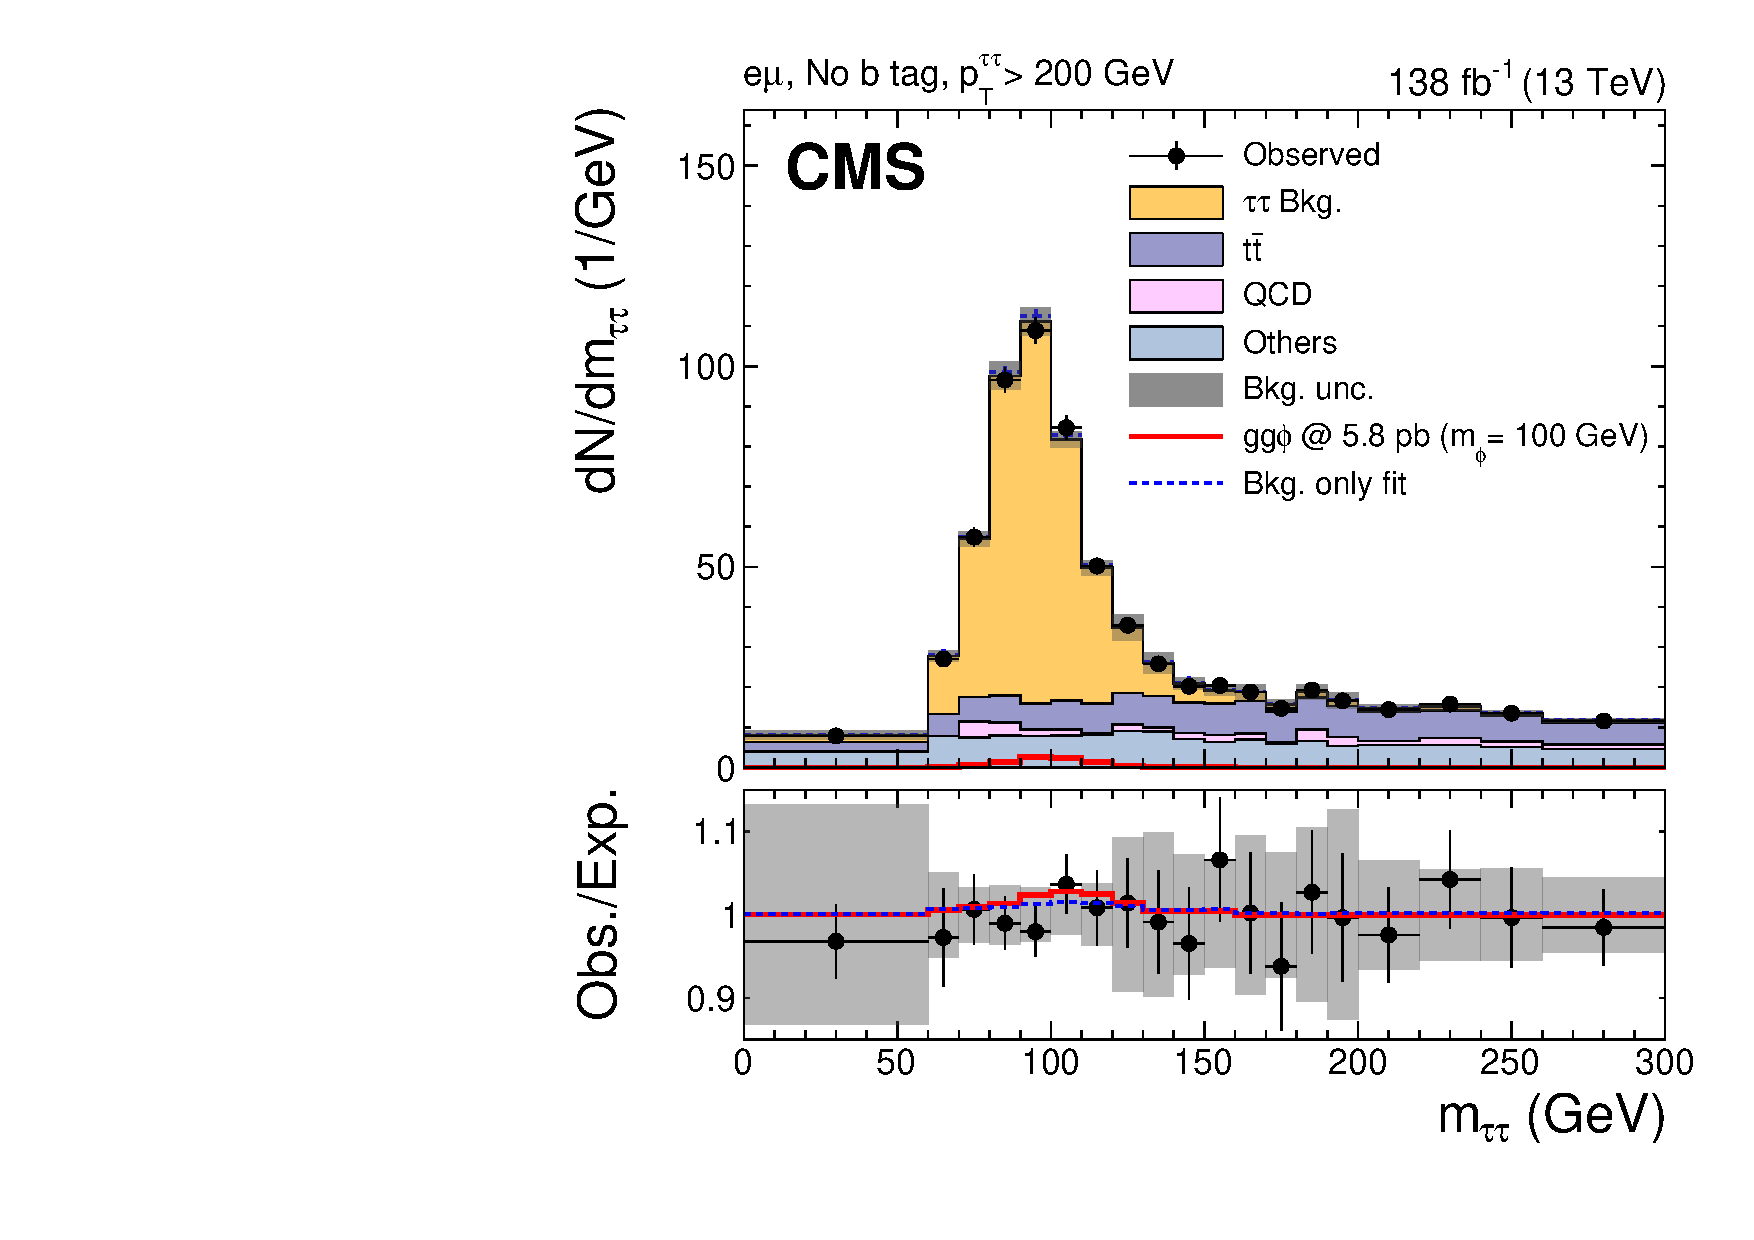
\includegraphics[width=0.45\textwidth]{Figures/postfit_lowmass_em_nobtag_highpT.pdf}}
\caption{Low mass postfit.}
\label{fig:low_mass_postfit}
\end{figure}

\begin{figure}[!hbtp]
\centering
    \subfloat[]{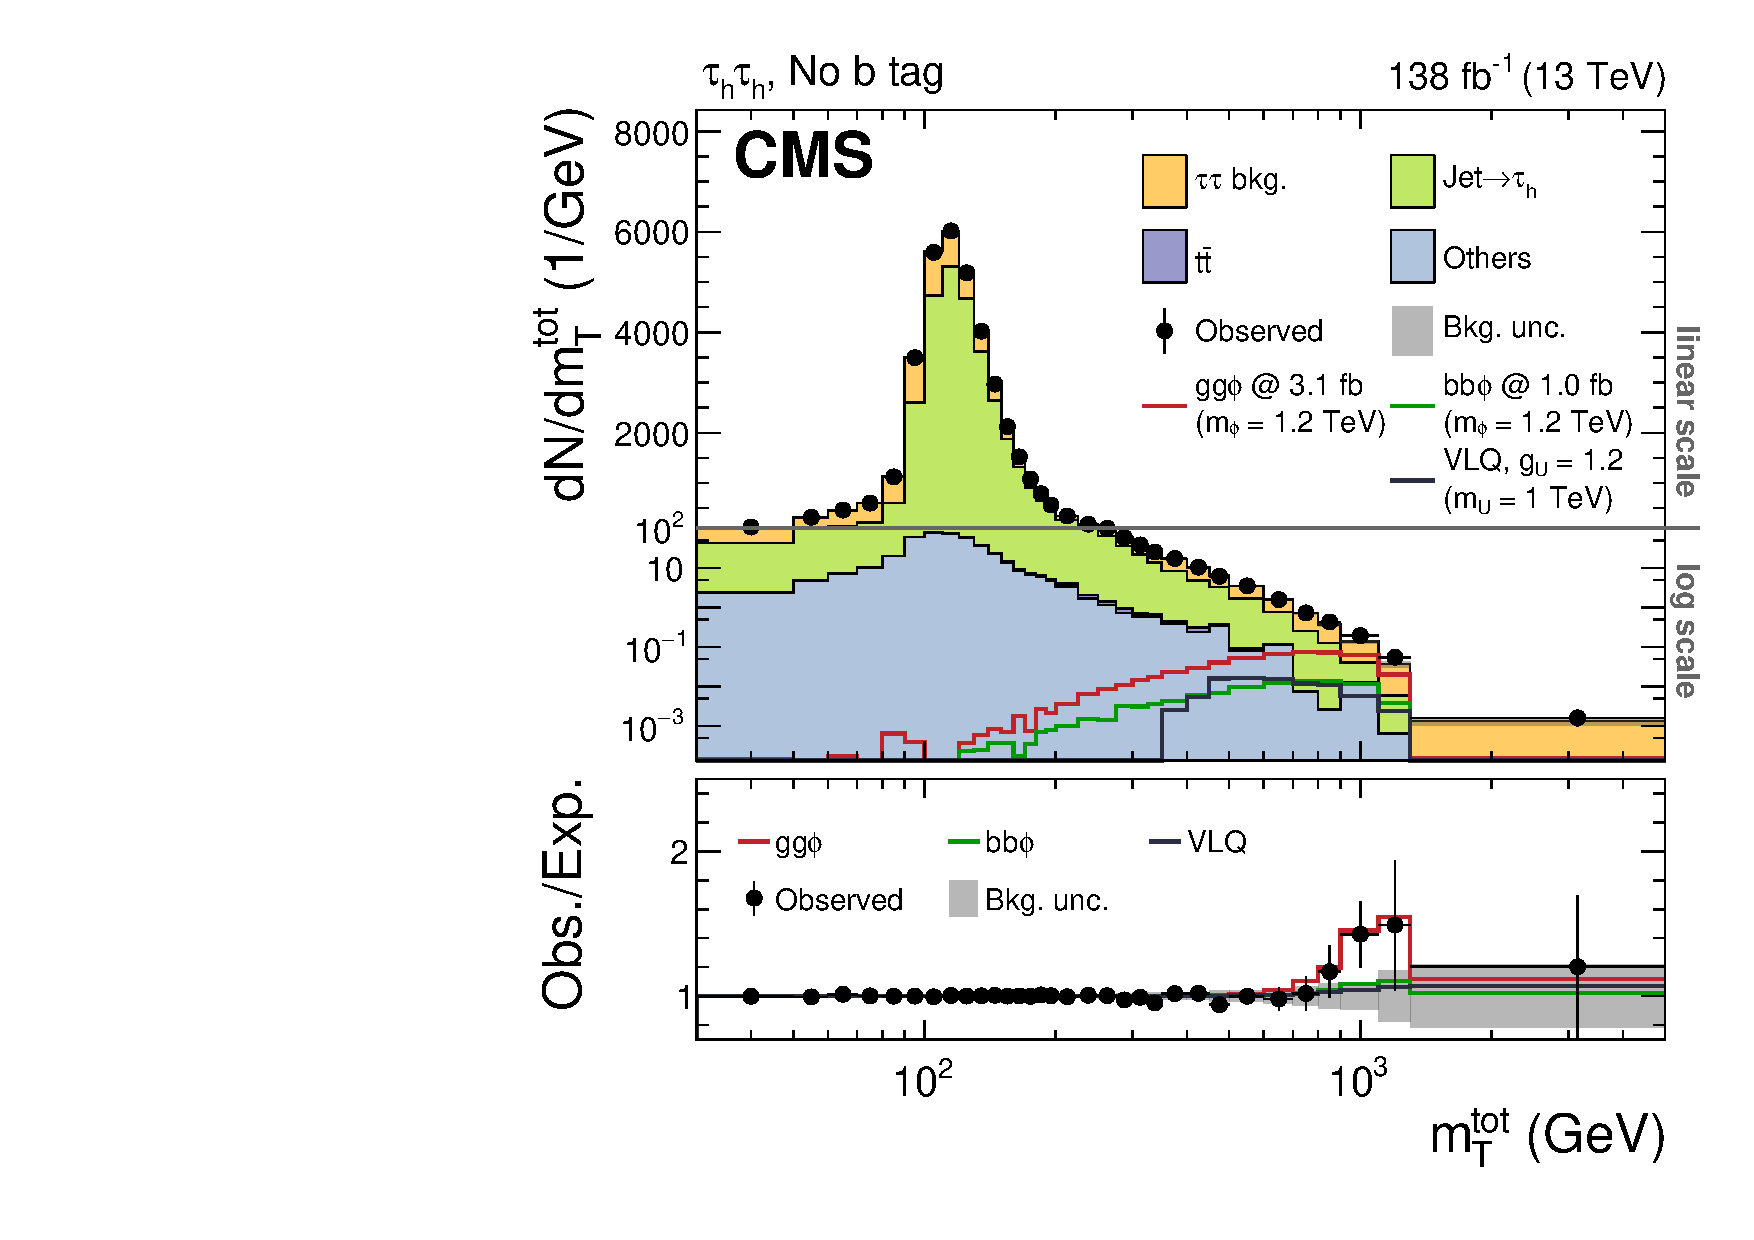
\includegraphics[width=0.45\textwidth]{Figures/postfit_highmass_tt_nobtag.pdf}}
    \subfloat[]{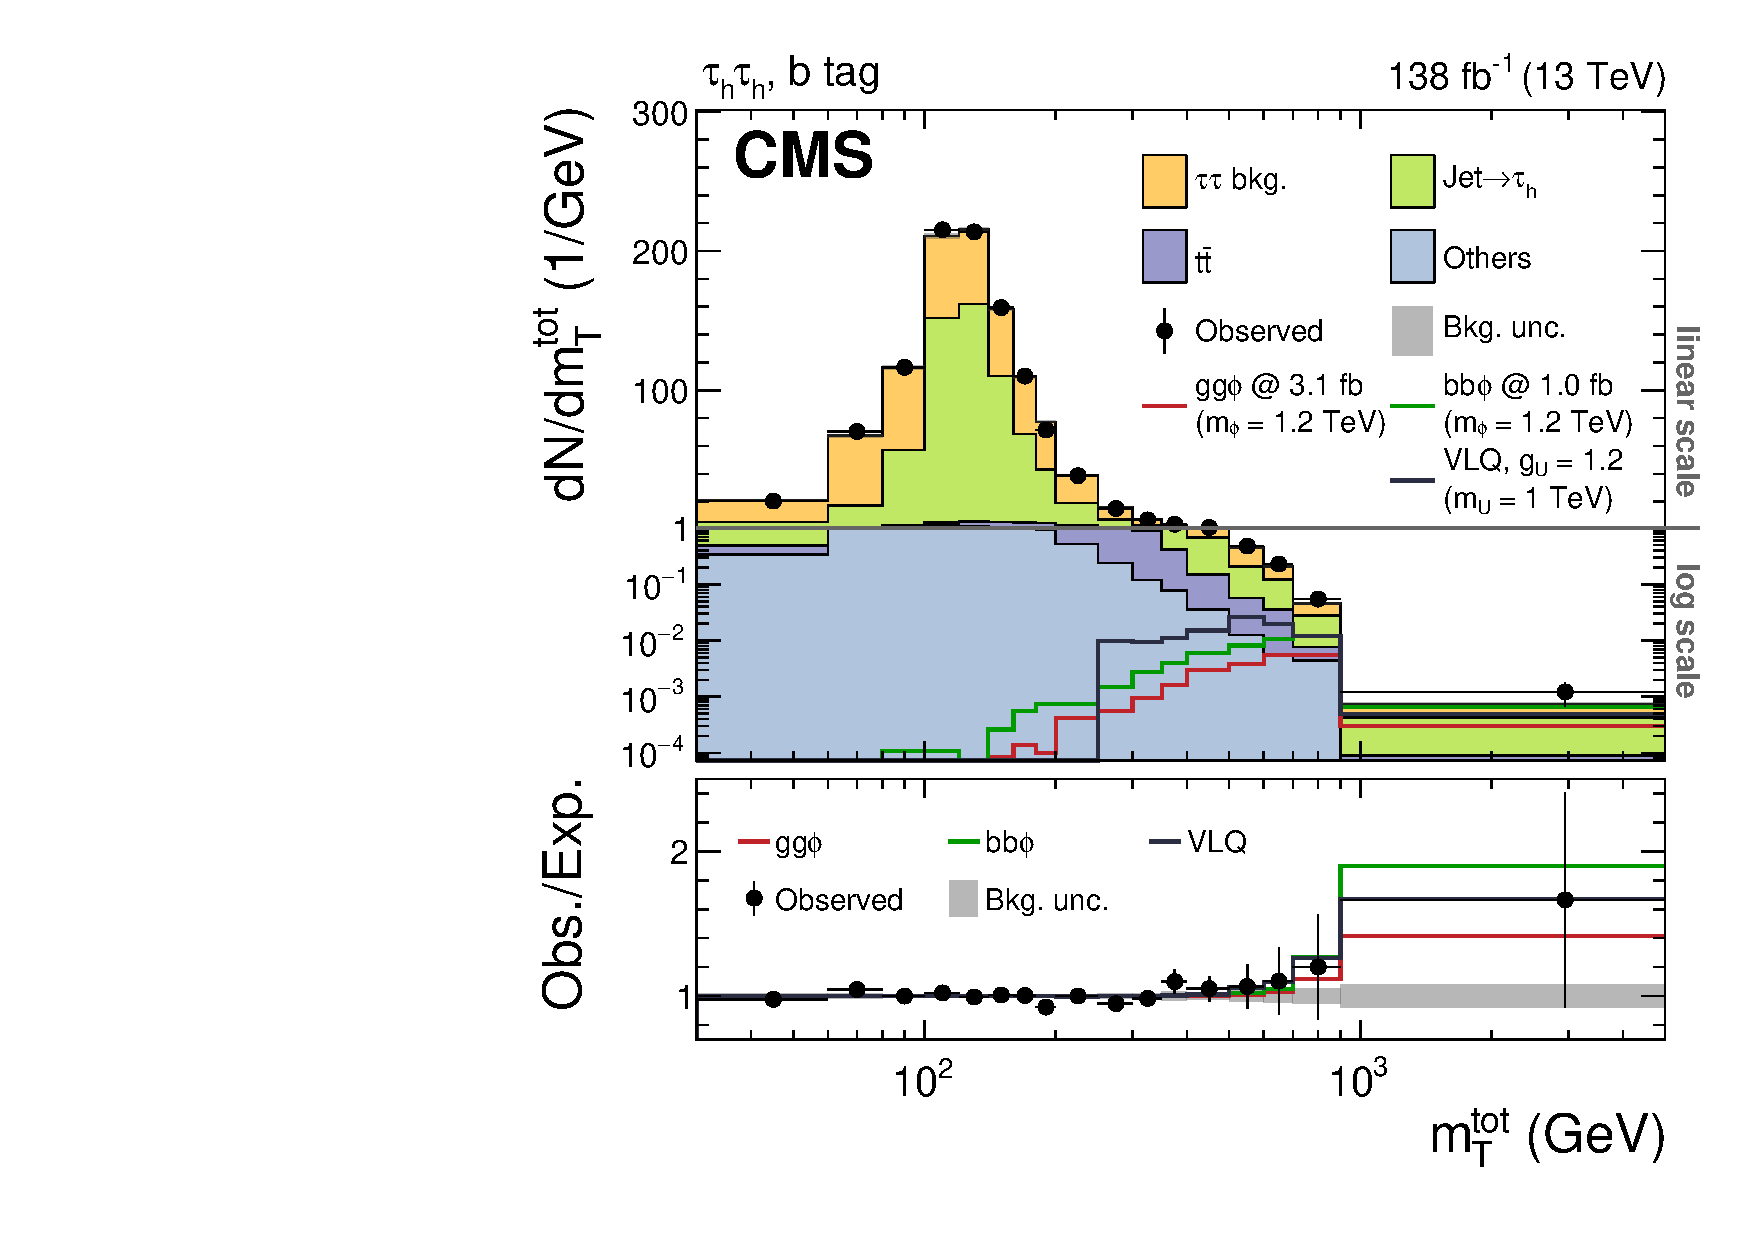
\includegraphics[width=0.45\textwidth]{Figures/postfit_highmass_tt_btag.pdf}} \\
    \subfloat[]{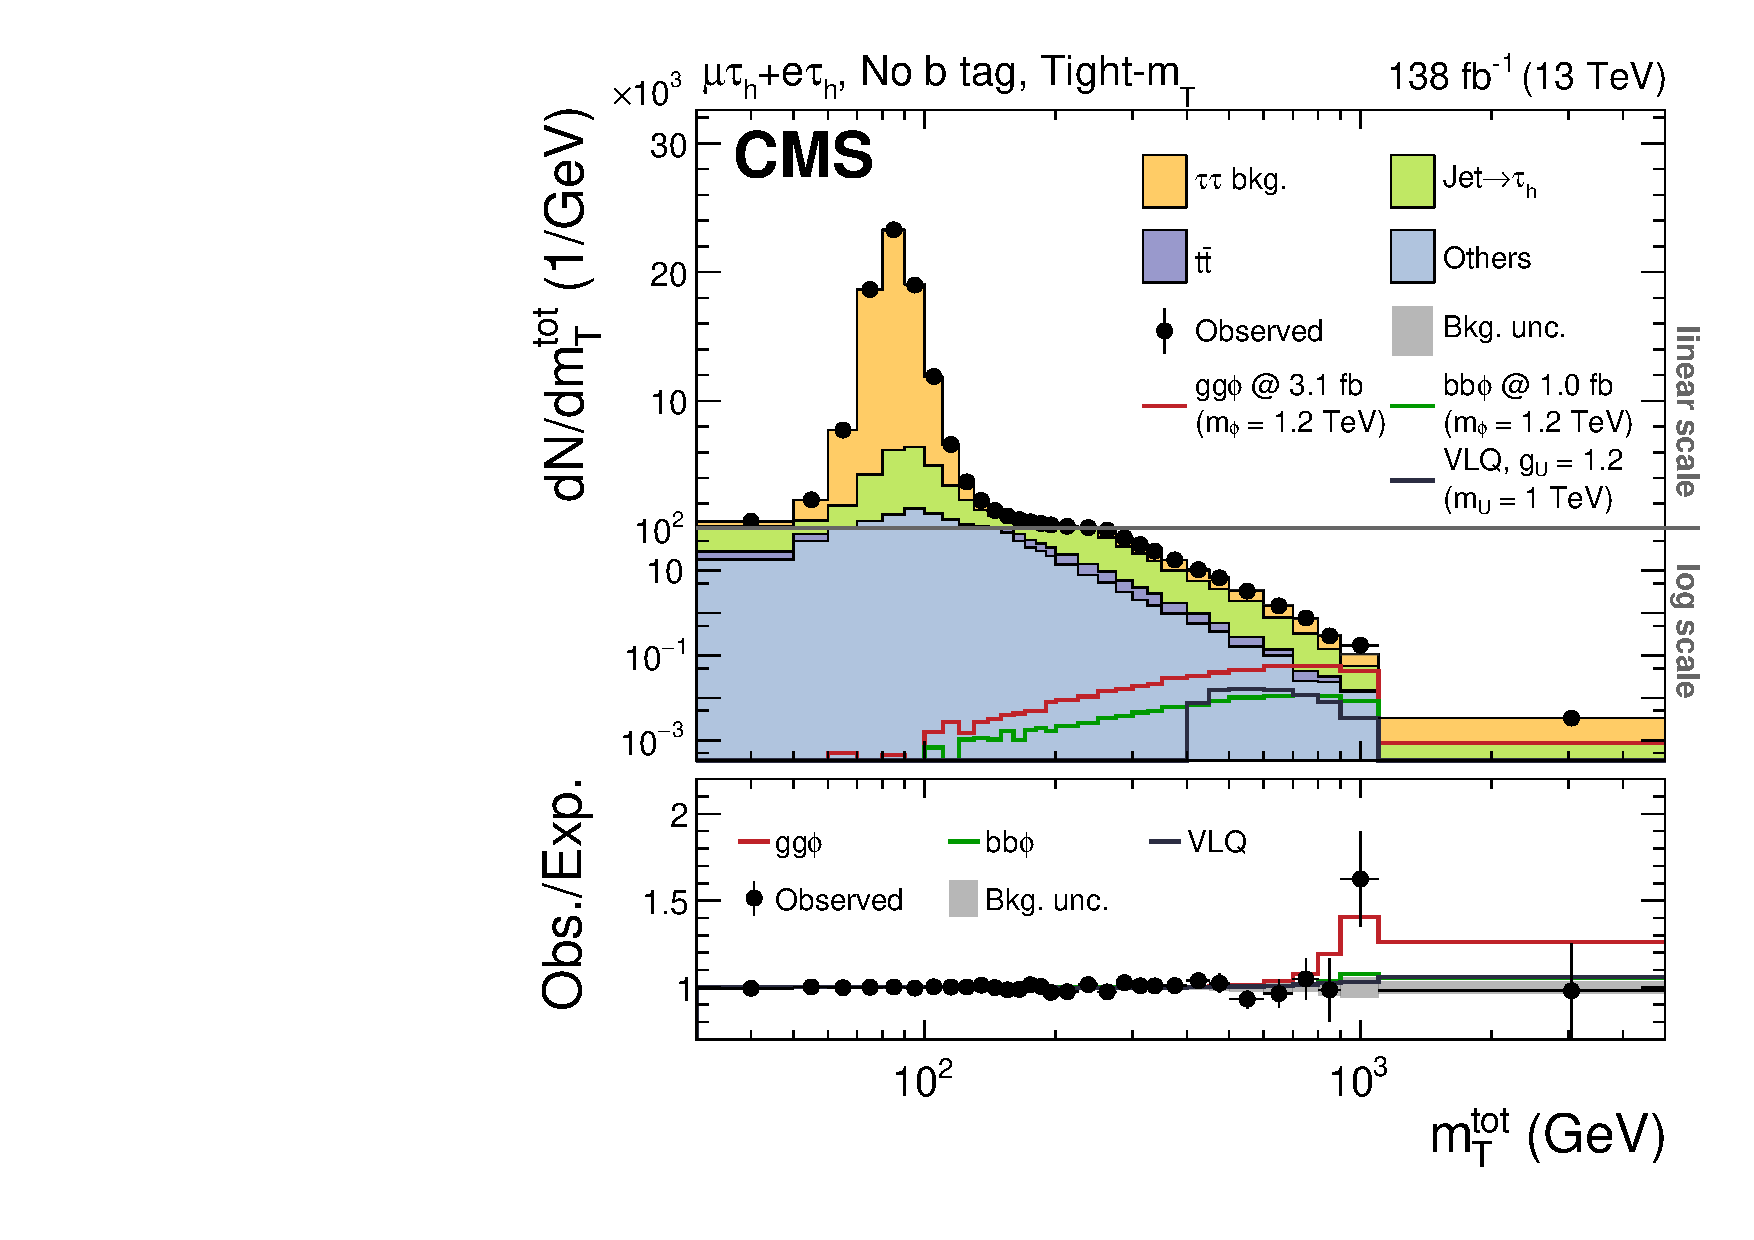
\includegraphics[width=0.45\textwidth]{Figures/postfit_highmass_lt_nobtag_tightmT.pdf}}
    \subfloat[]{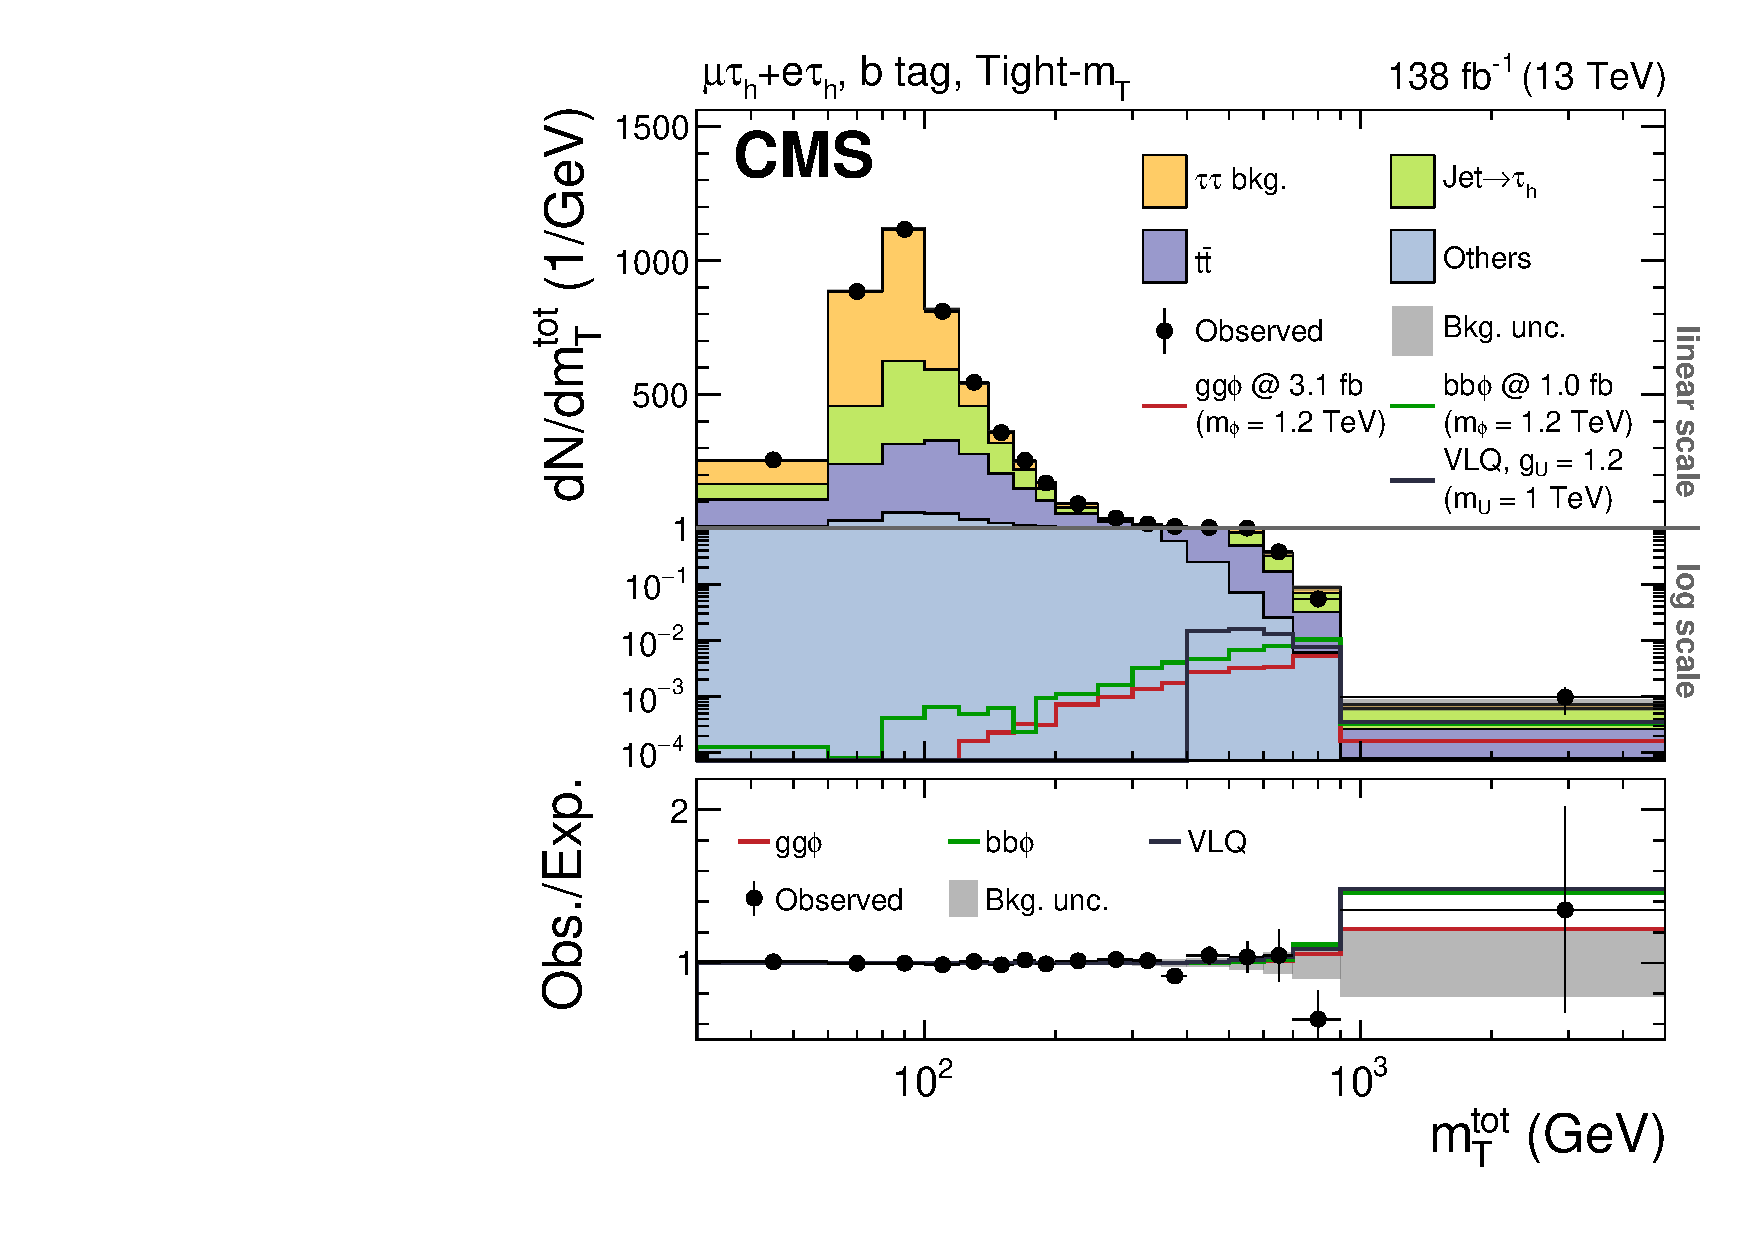
\includegraphics[width=0.45\textwidth]{Figures/postfit_highmass_lt_btag_tightmT.pdf}} \\
    \subfloat[]{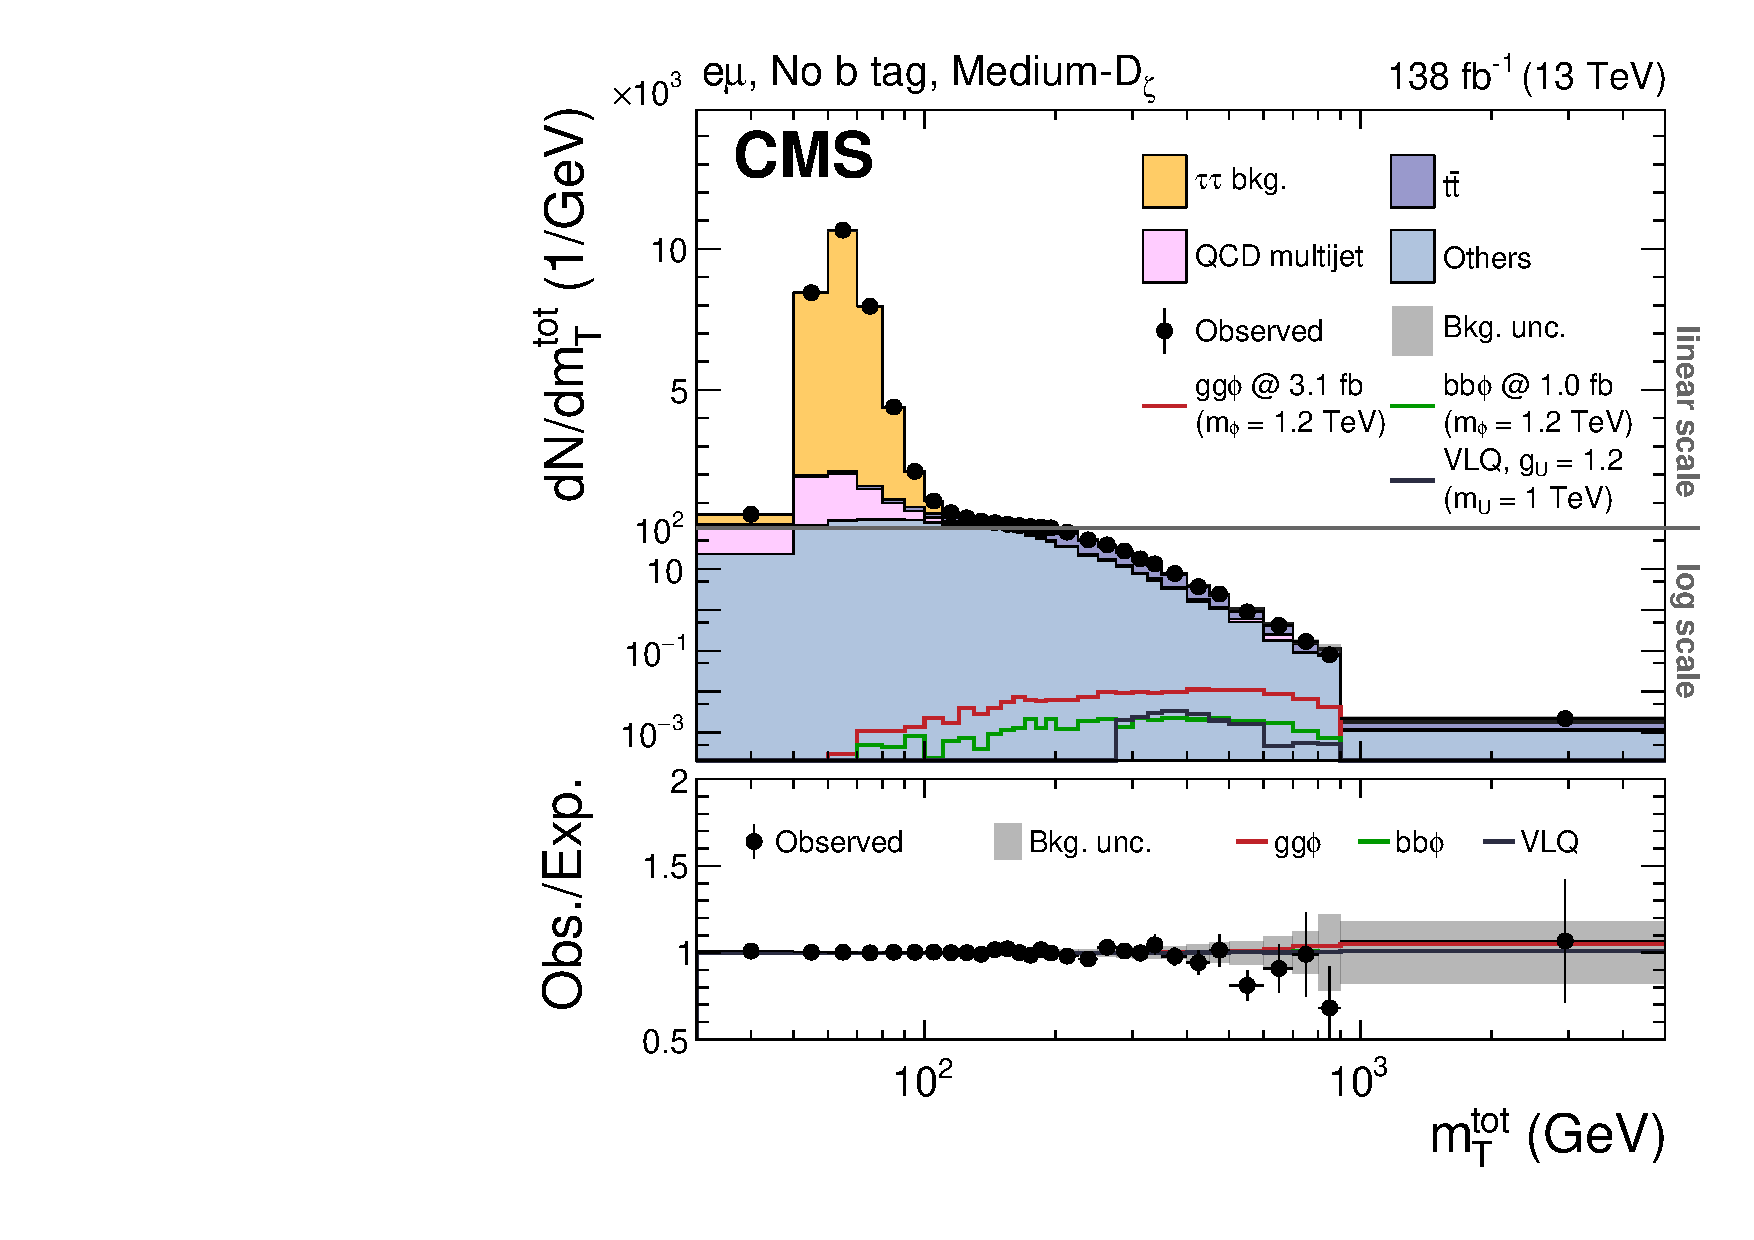
\includegraphics[width=0.45\textwidth]{Figures/postfit_highmass_em_nobtag_mediumdzeta.pdf}}
    \subfloat[]{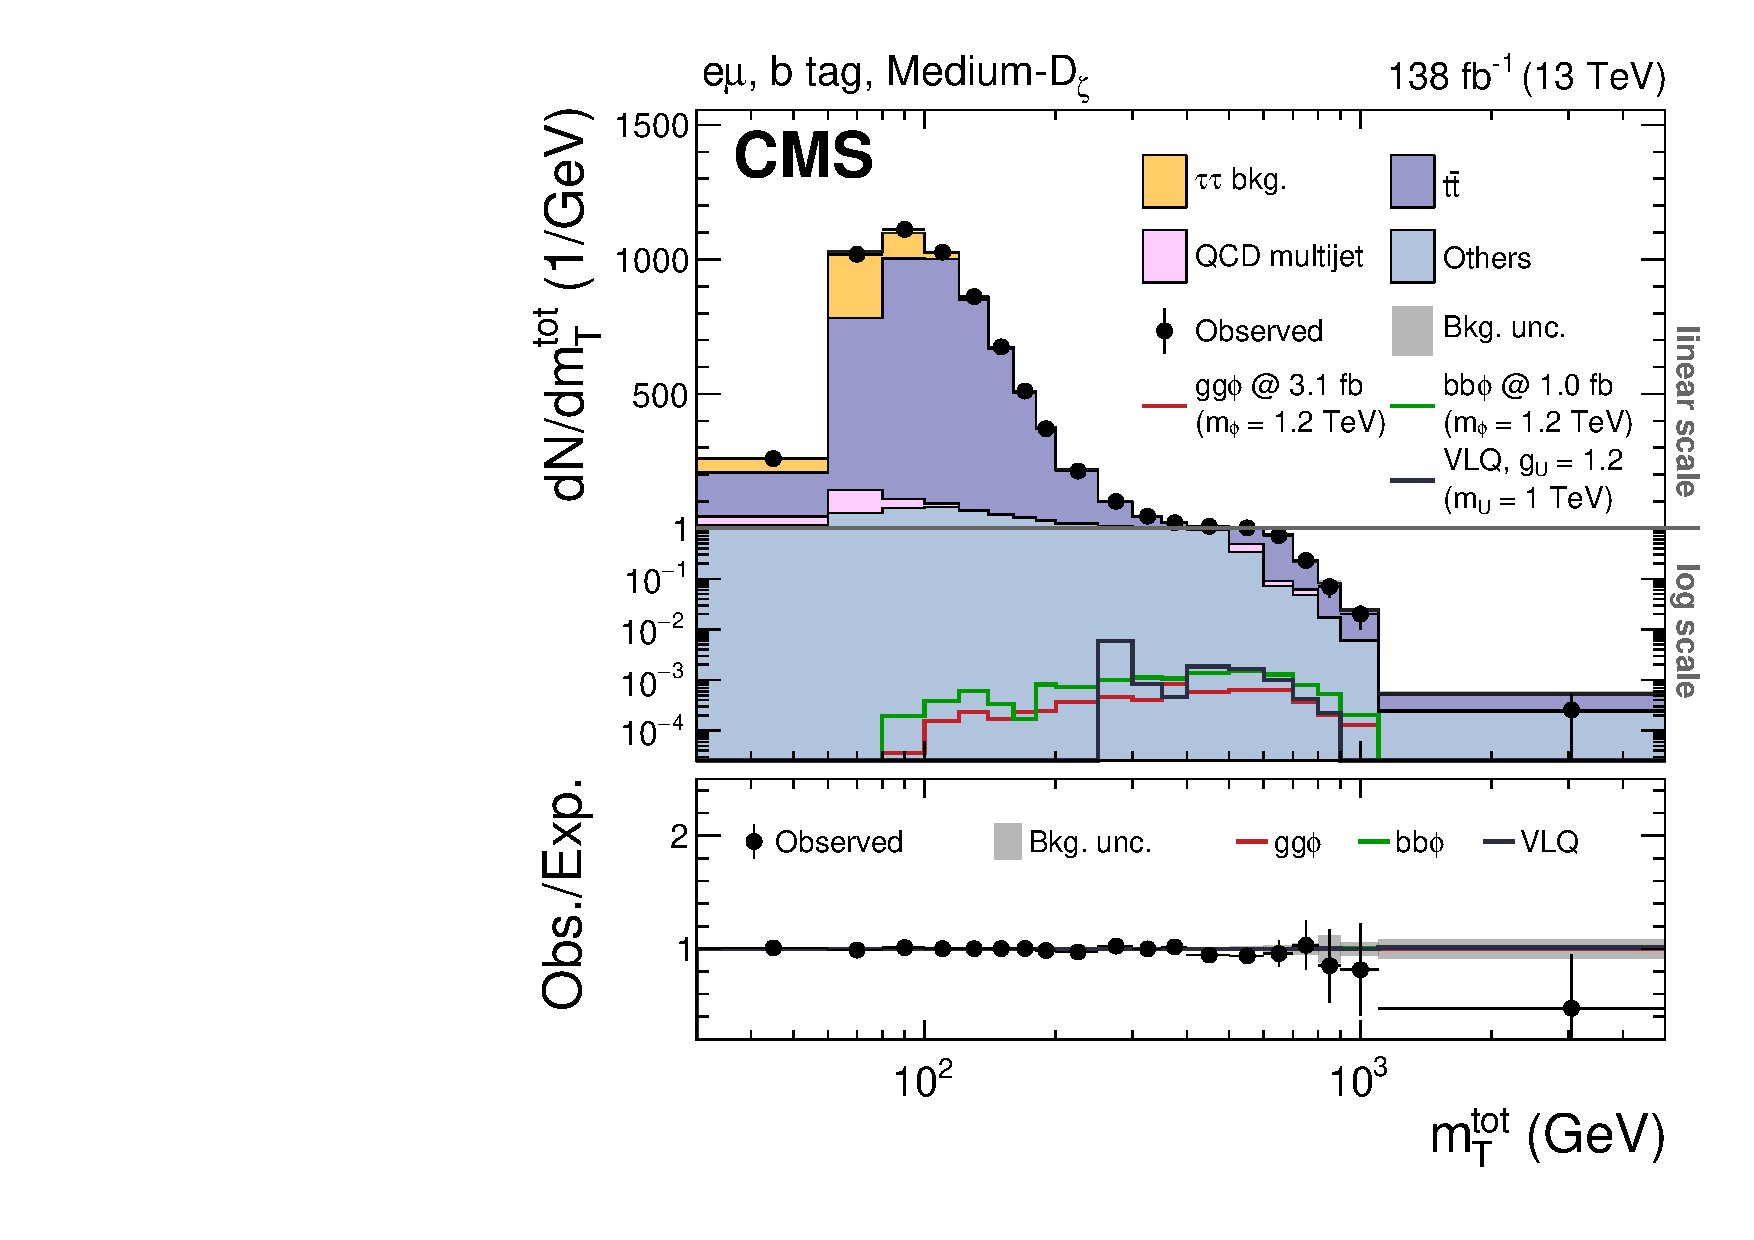
\includegraphics[width=0.45\textwidth]{Figures/postfit_highmass_em_btag_mediumdzeta.pdf}}
\caption{High mass postfit.}
\label{fig:high_mass_postfit}
\end{figure}

\section{MC Corrections}

\section{Model Independent Results}

\subsection{Limit Setting}

\begin{equation}
  q_{\mu} = -2 \ln \Biggl(\frac{\mathcal{L}(\text{data} | \mu, \hat{\theta}_{\mu})}{\mathcal{L}(\text{data} | \hat{\mu}, \hat{\theta}_{\hat{\mu}})}\Biggl), 0 \leq \hat{\mu} \leq \mu,
\end{equation}

\begin{figure}[!hbtp]
\centering
    \subfloat[]{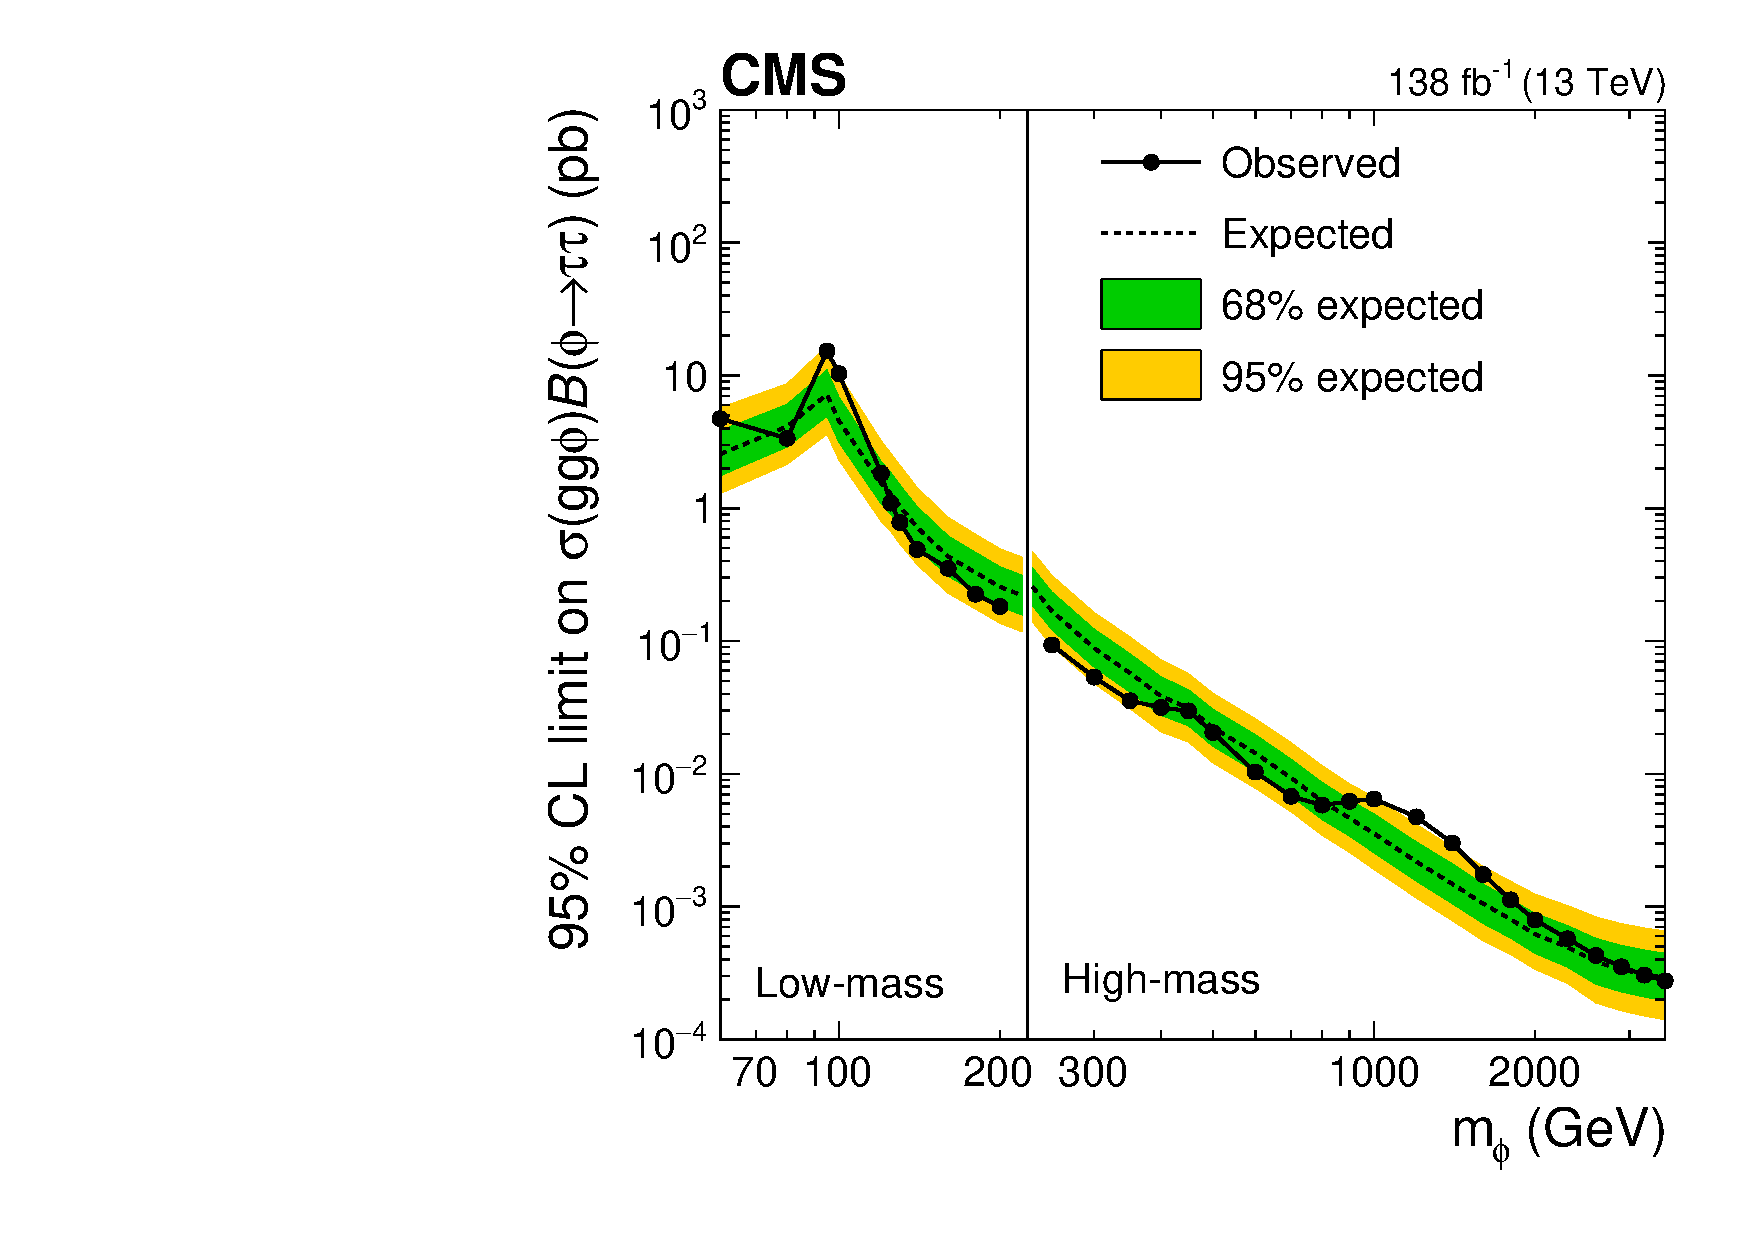
\includegraphics[width=0.5\textwidth]{Figures/model_independent_limit_ggH.pdf}}
    \subfloat[]{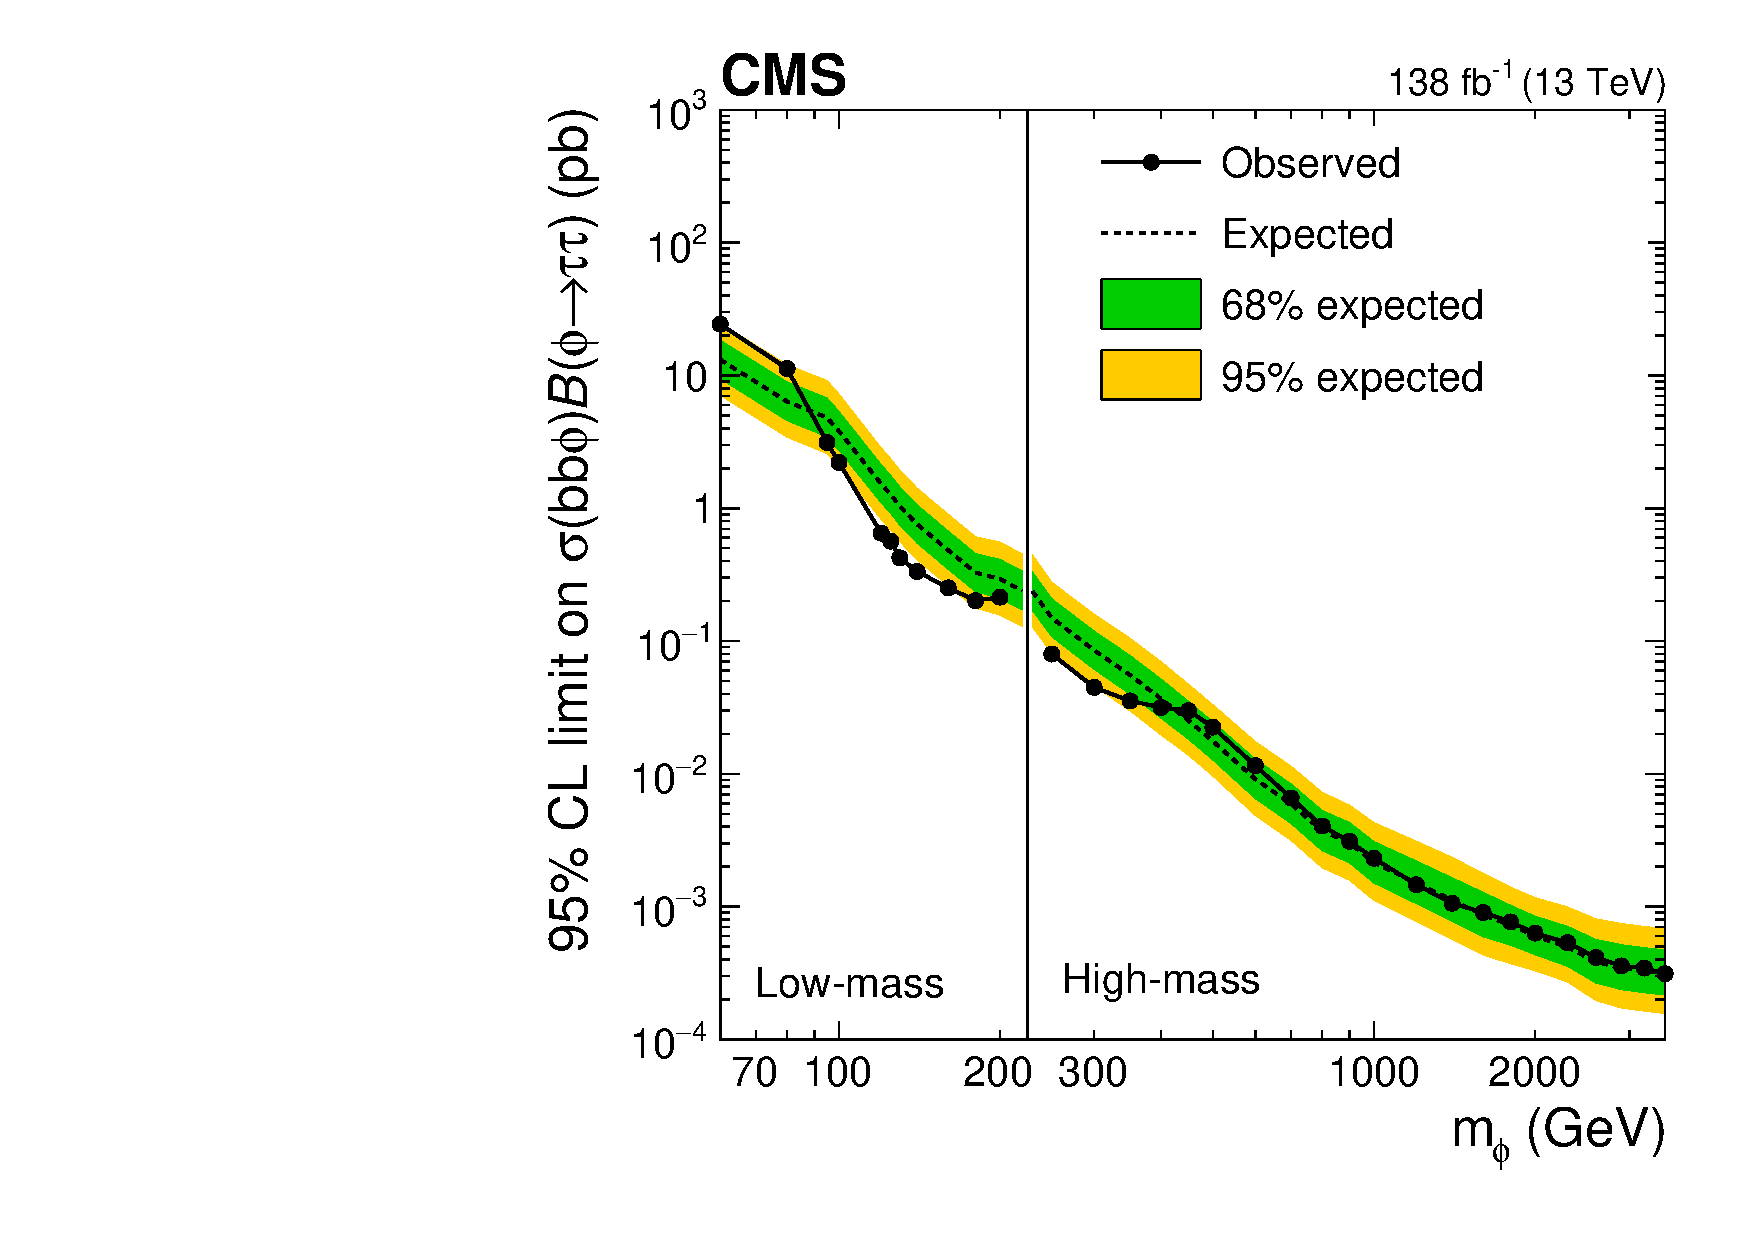
\includegraphics[width=0.5\textwidth]{Figures/model_independent_limit_bbH.pdf}}
\caption{Model independent limits.}
\label{fig:model_independent_limits}
\end{figure}

\begin{figure}[!hbtp]
\centering
    \subfloat[]{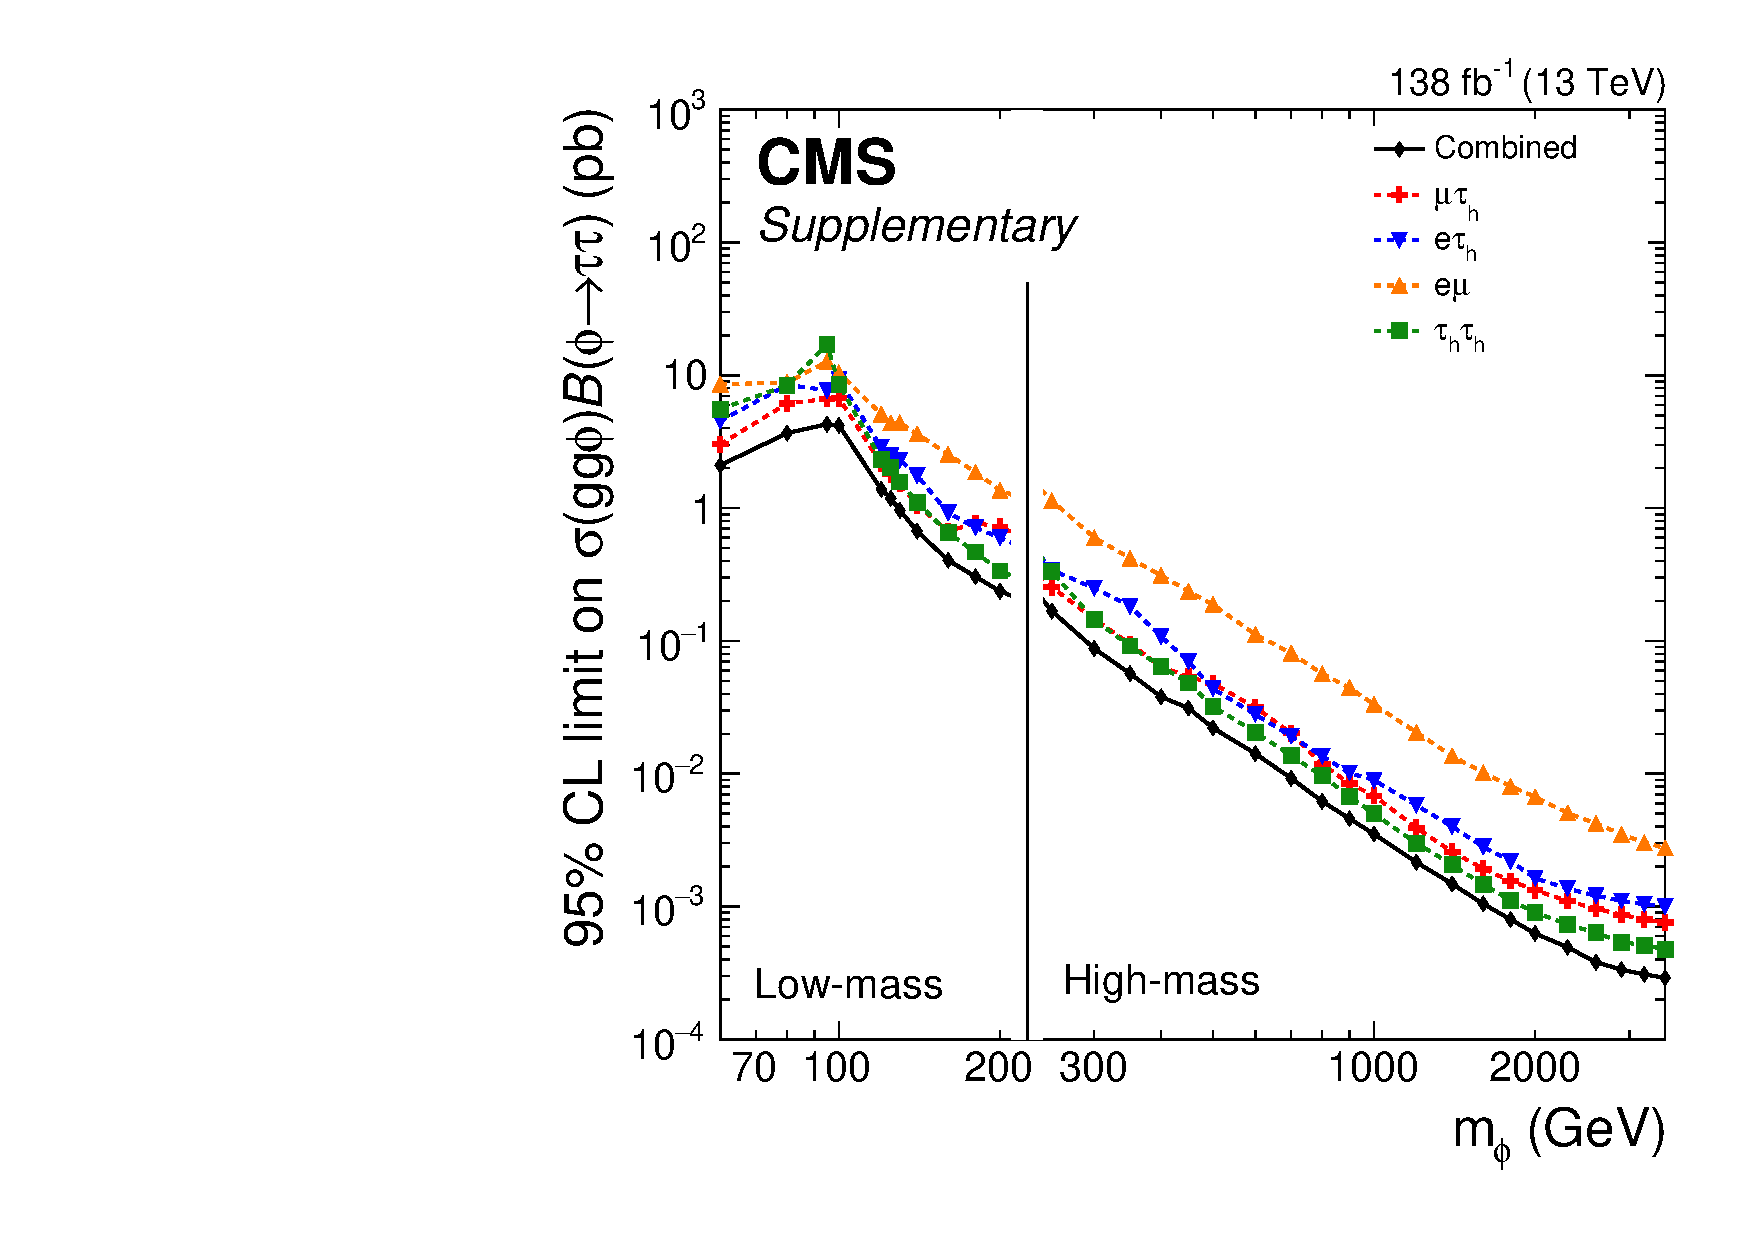
\includegraphics[width=0.5\textwidth]{Figures/limit_comparison_mssm_ggphi.pdf}}
    \subfloat[]{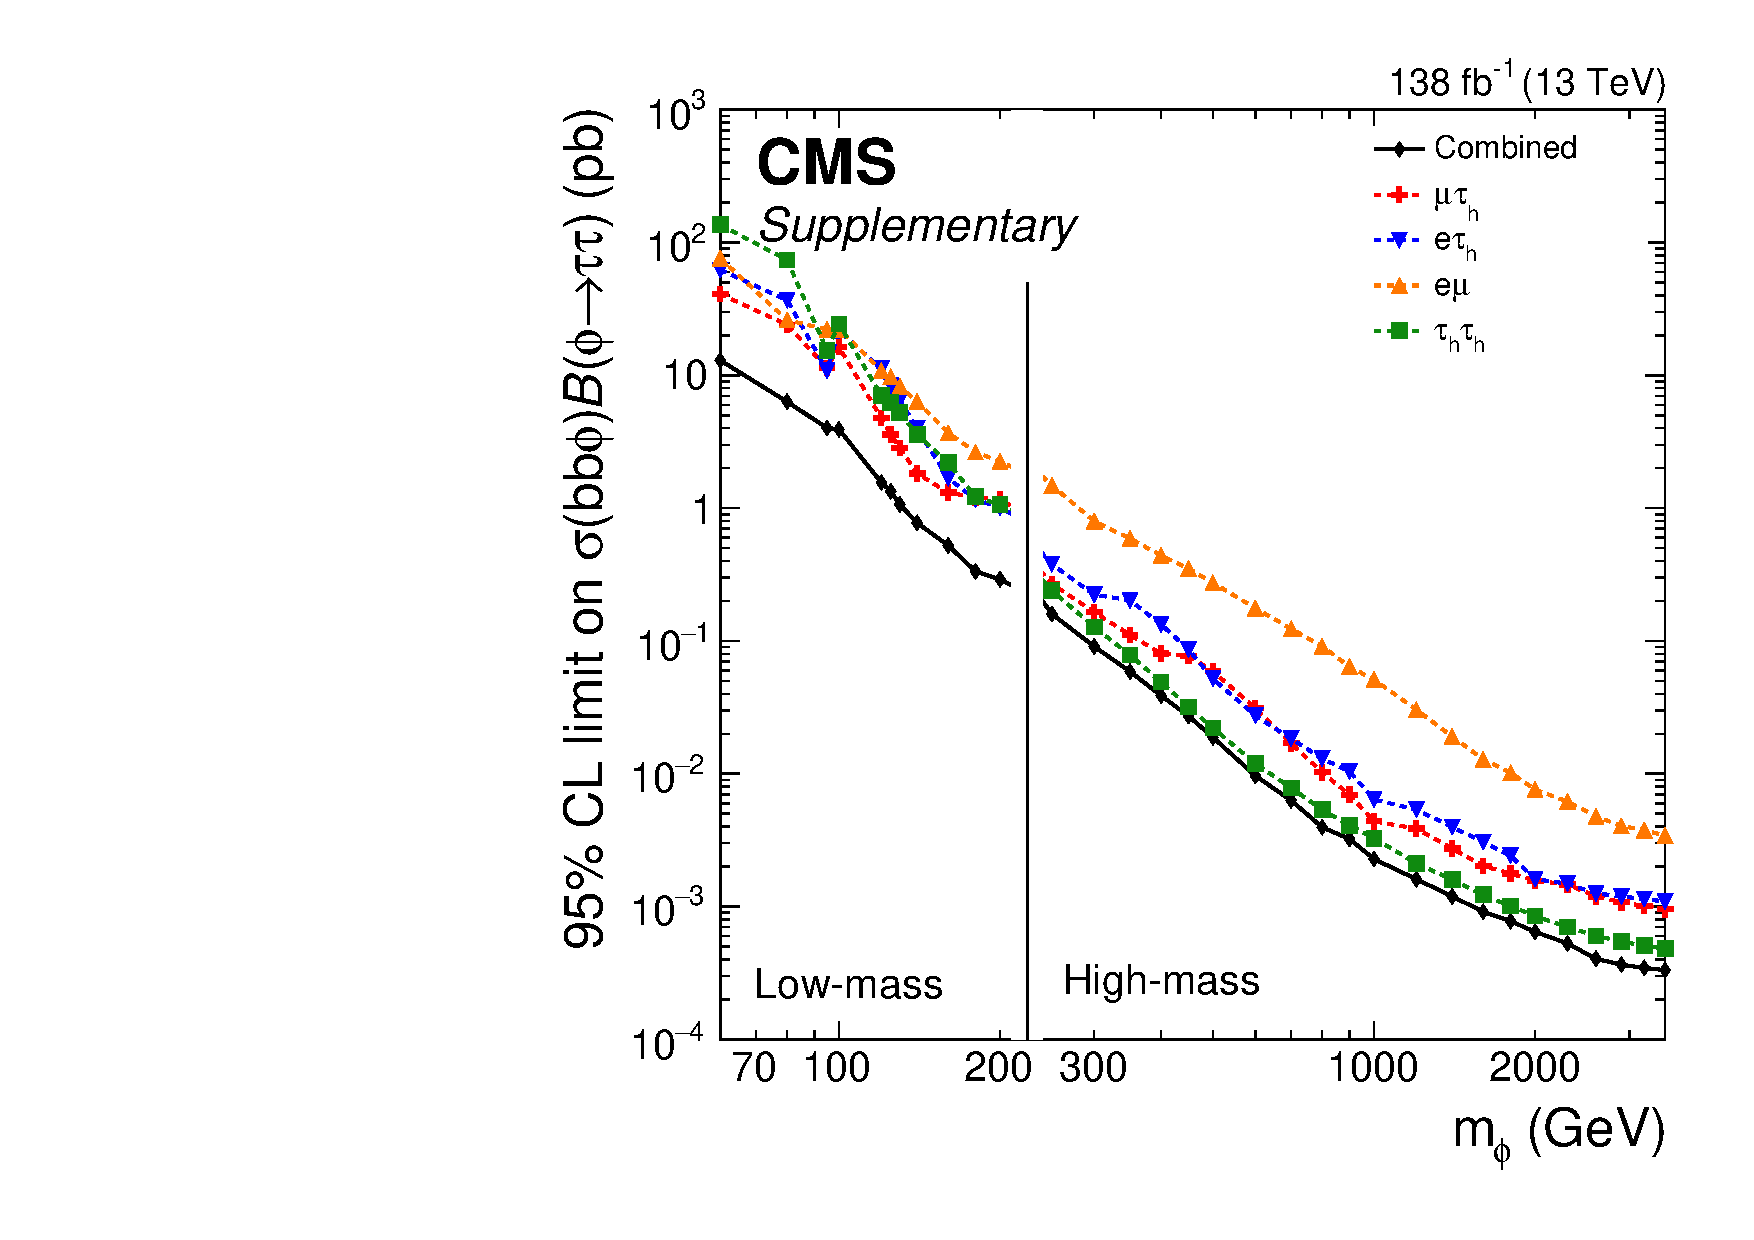
\includegraphics[width=0.5\textwidth]{Figures/limit_comparison_mssm_bbphi.pdf}}
\caption{Model independent limits.}
\label{fig:model_independent_limits_by_channel}
\end{figure}

\begin{figure}[!hbtp]
\centering
    \subfloat[]{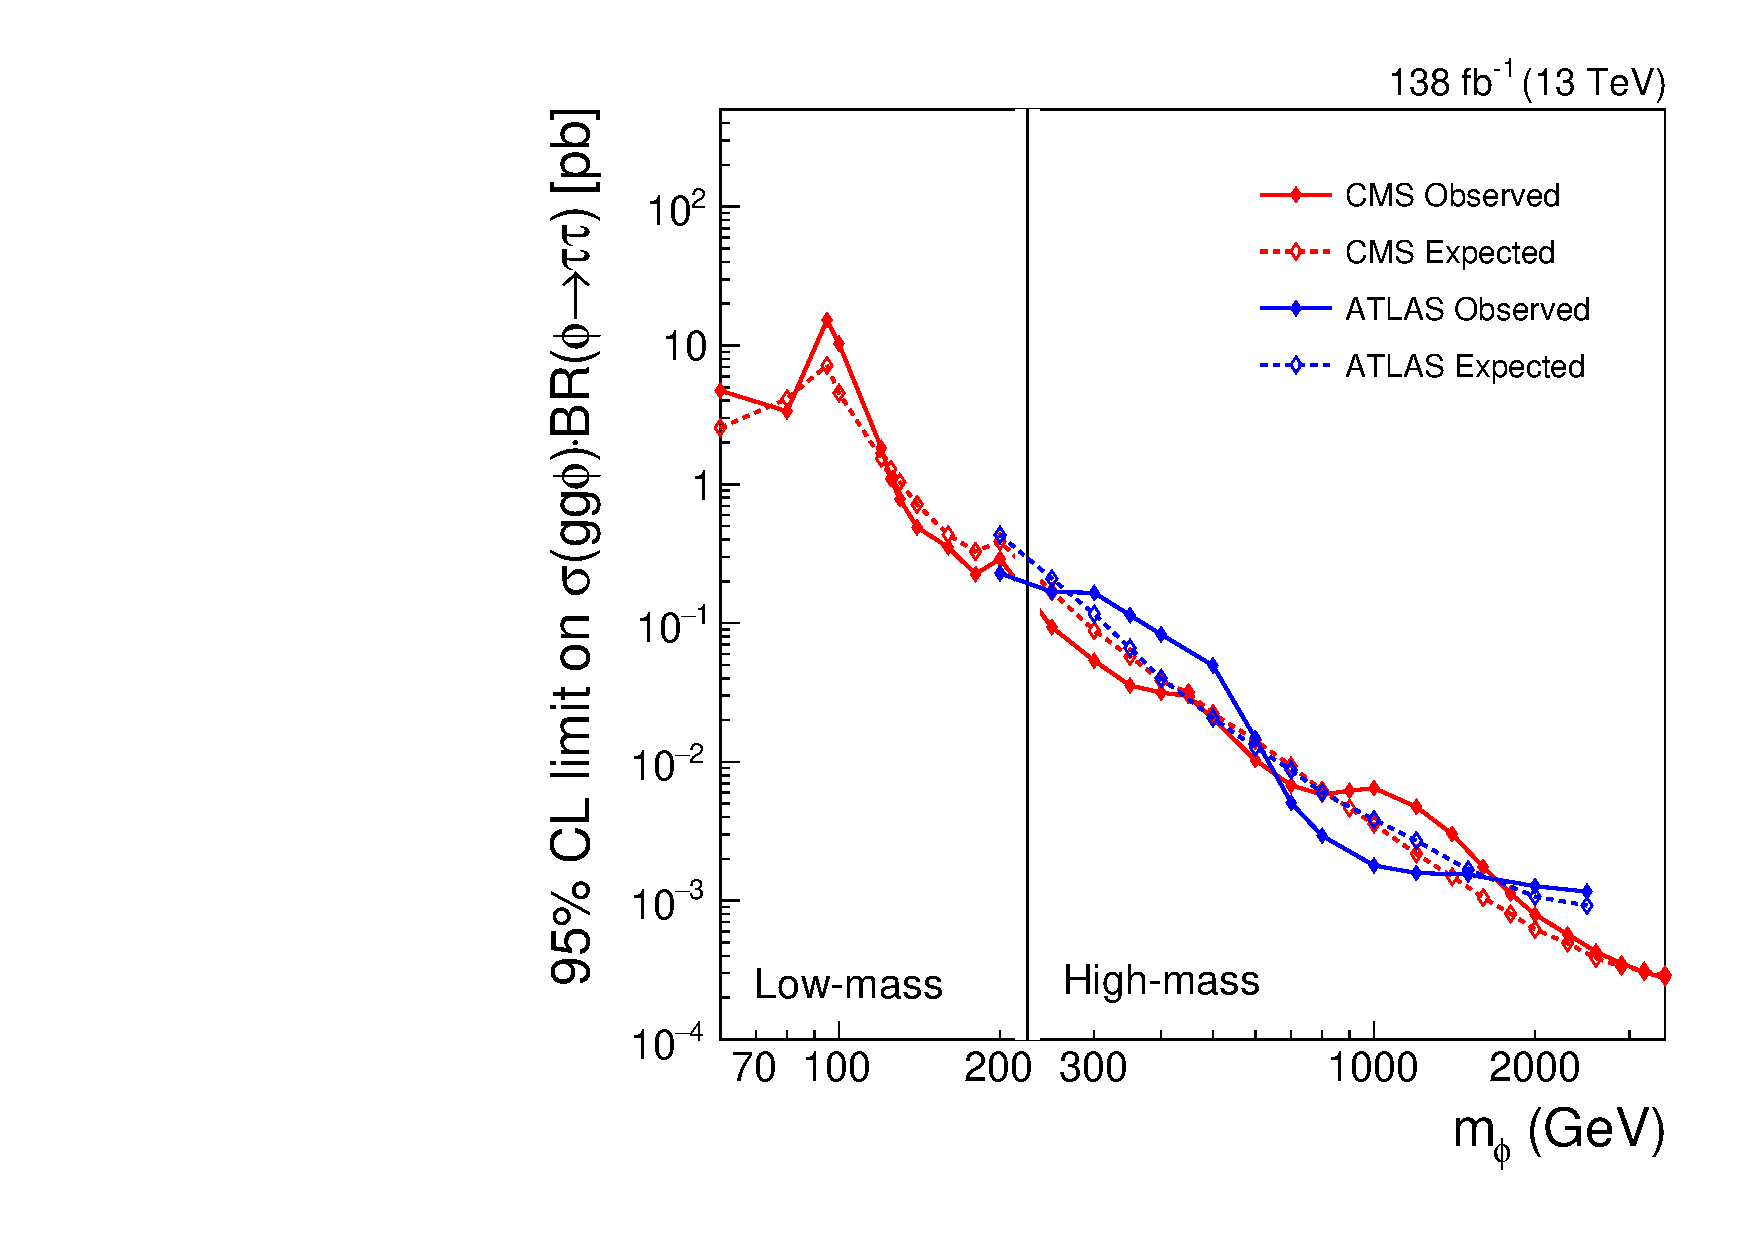
\includegraphics[width=0.5\textwidth]{Figures/limit_comparison_gg_ATLAS.pdf}}
    \subfloat[]{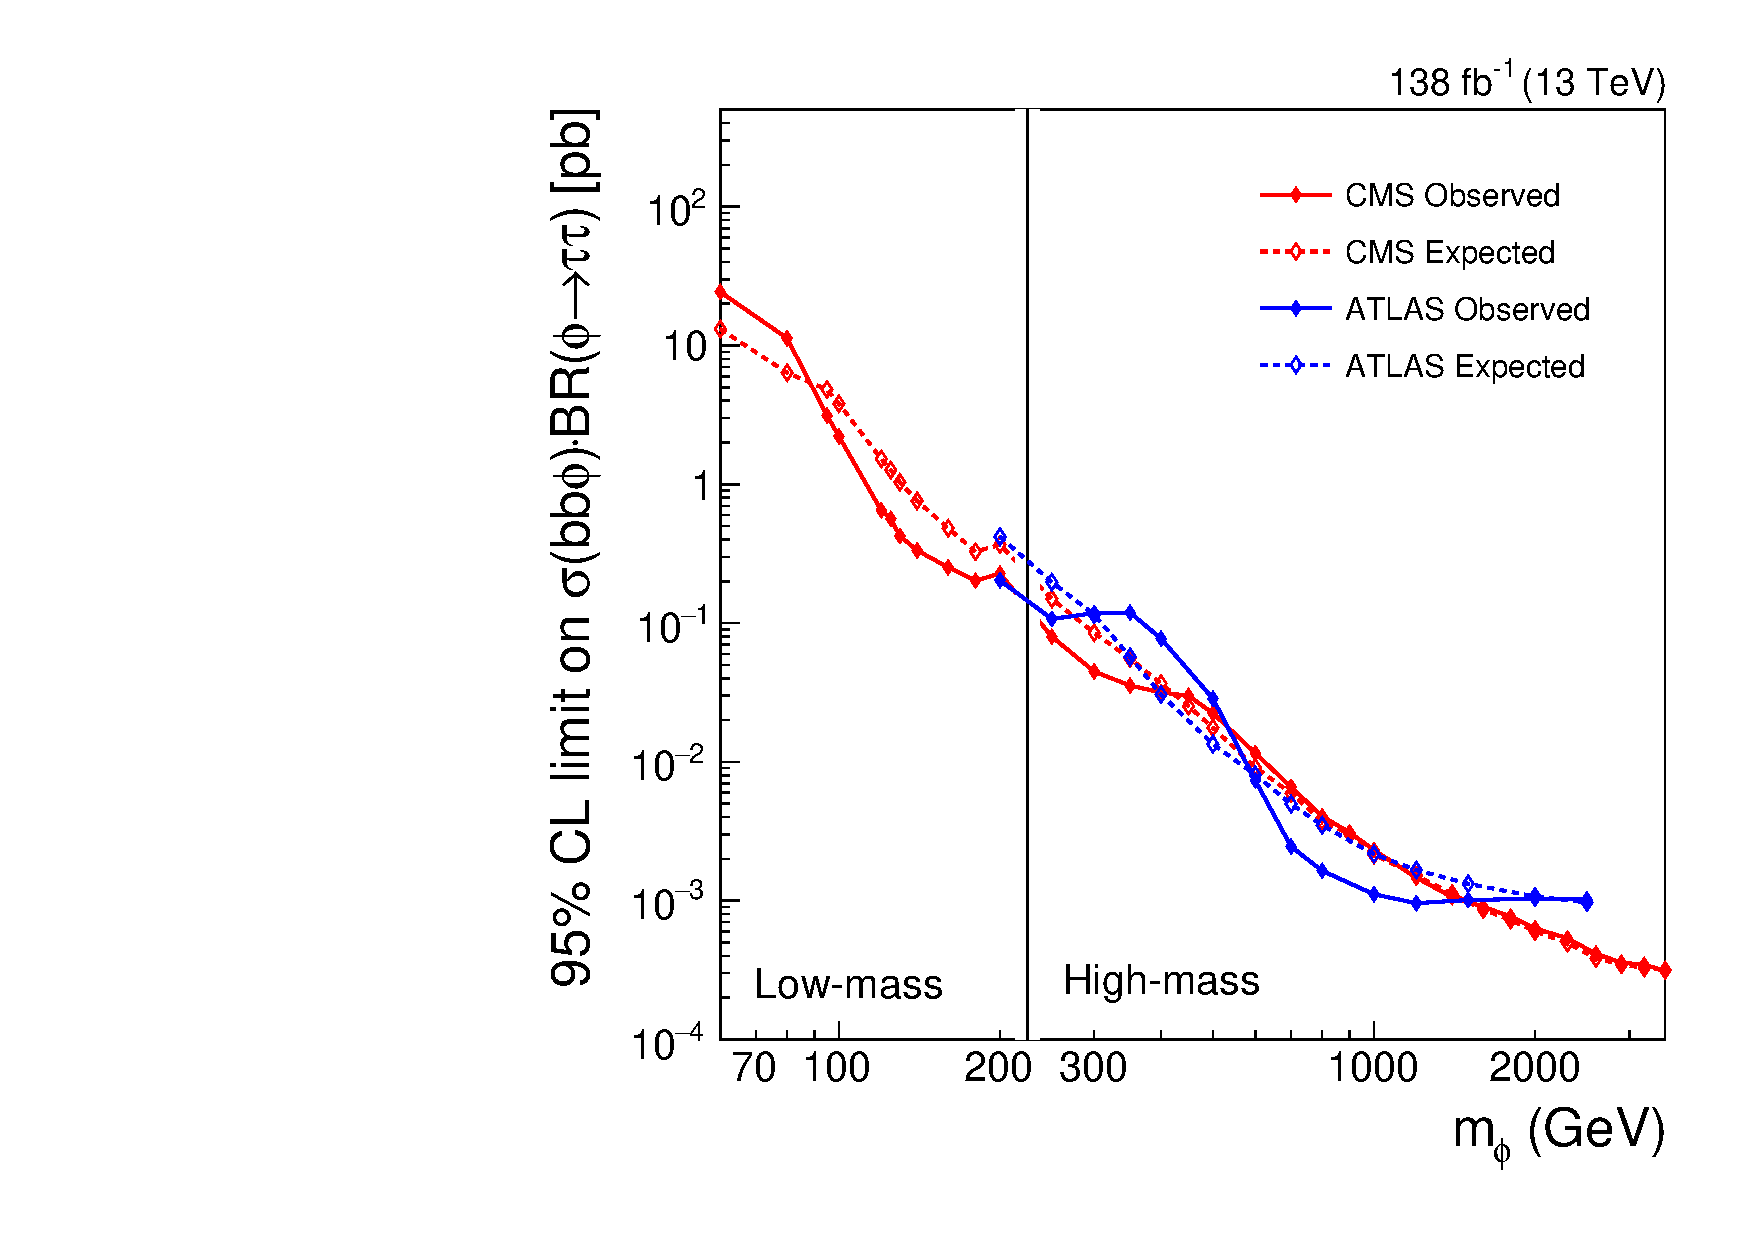
\includegraphics[width=0.5\textwidth]{Figures/limit_comparison_bb_ATLAS.pdf}}
\caption{Model independent limits.}
\label{fig:model_independent_limits_by_channel}
\end{figure}

\subsection{Significance and Compatibility}

\begin{figure}[!hbtp]
\centering
    \subfloat[]{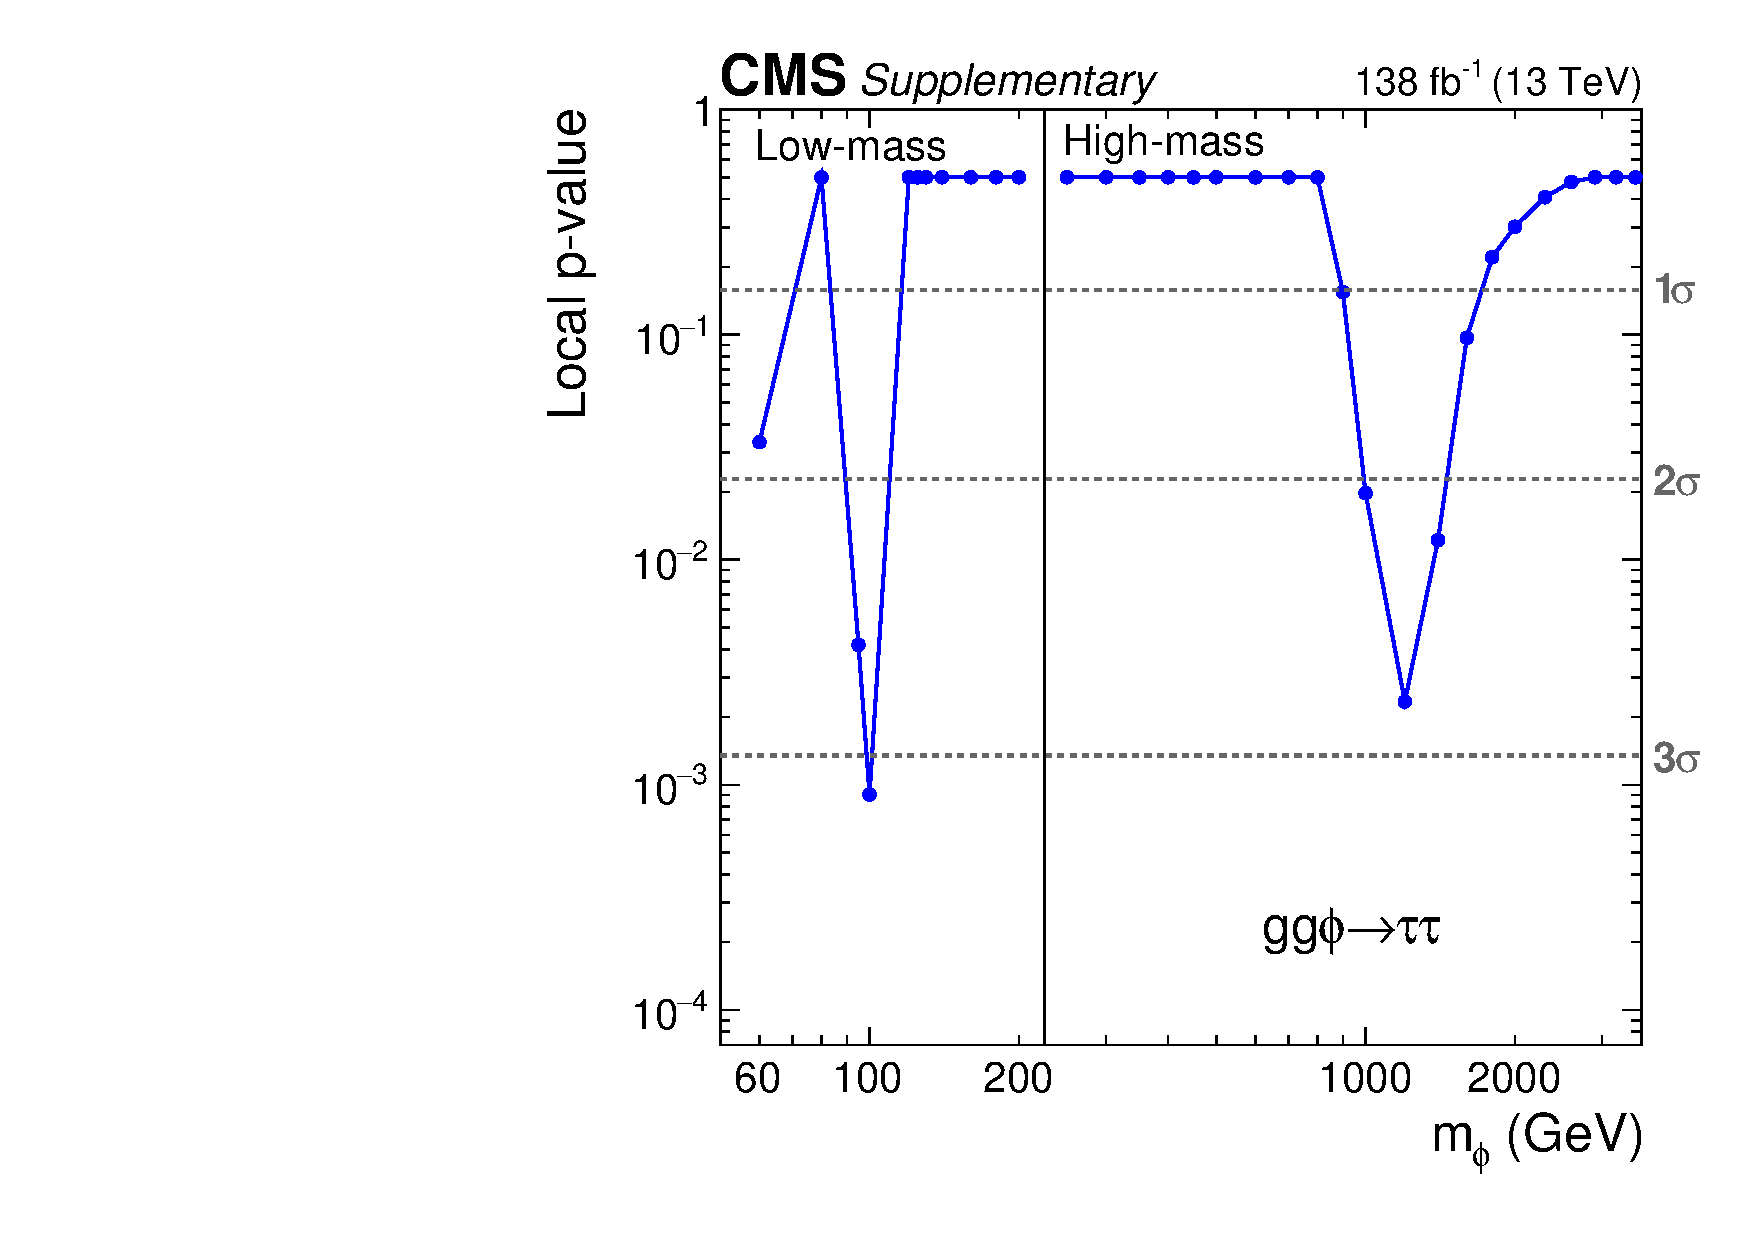
\includegraphics[width=0.5\textwidth]{Figures/significance_plot_ggH.pdf}}
    \subfloat[]{\includegraphics[width=0.5\textwidth]{Figures/significance_plot_bbH.pdf}}
\caption{Significance.}
\label{fig:significance}
\end{figure}

\begin{figure}[!hbtp]
\centering
    \subfloat[]{\includegraphics[width=0.5\textwidth]{Figures/ChannelCompatibilityCheck_FitResults_mH100_channel.pdf}}
    \subfloat[]{\includegraphics[width=0.5\textwidth]{Figures/ChannelCompatibilityCheck_FitResults_mH100_cat.pdf}}
\caption{Low mass compatibility.}
\label{fig:low_mass_compatibility}
\end{figure}

\begin{figure}[!hbtp]
\centering
    \includegraphics[width=0.5\textwidth]{Figures/ccc_fit_result_mH1200_per-channel.pdf}
\caption{High mass compatibility.}
\label{fig:high_mass_compatibility}
\end{figure}

\subsection{2D Likelihood Scans}

\begin{figure}[!hbtp]
\centering
    \subfloat[]{\includegraphics[width=0.33\textwidth]{Figures/2d_lkld_60.pdf}}
    \subfloat[]{\includegraphics[width=0.33\textwidth]{Figures/2d_lkld_100.pdf}}
    \subfloat[]{\includegraphics[width=0.33\textwidth]{Figures/2d_lkld_125.pdf}} \\
    \subfloat[]{\includegraphics[width=0.33\textwidth]{Figures/2d_lkld_160.pdf}}
    \subfloat[]{\includegraphics[width=0.33\textwidth]{Figures/2d_lkld_250.pdf}}
    \subfloat[]{\includegraphics[width=0.33\textwidth]{Figures/2d_lkld_500.pdf}} \\
    \subfloat[]{\includegraphics[width=0.33\textwidth]{Figures/2d_lkld_1000.pdf}}
    \subfloat[]{\includegraphics[width=0.33\textwidth]{Figures/2d_lkld_1200.pdf}}
    \subfloat[]{\includegraphics[width=0.33\textwidth]{Figures/2d_lkld_3500.pdf}}
\caption{2D Likelihood scans.}
\label{fig:2d_likelihood_scans}
\end{figure}

\section{Model Dependent Limits}

\subsection{Limit Setting}

\begin{figure}[!hbtp]
\centering
    \subfloat[]{\includegraphics[width=0.5\textwidth]{Figures/model-dependent_limit_mh125.pdf}}
    \subfloat[]{\includegraphics[width=0.5\textwidth]{Figures/model-dependent_limit_mh125EFT.pdf}}
\caption{MSSM limits.}
\label{fig:mssm_limits}
\end{figure}

\begin{figure}[!hbtp]
\centering
    \subfloat[]{\includegraphics[width=0.5\textwidth]{Figures/vlq_bm_1.pdf}}
    \subfloat[]{\includegraphics[width=0.5\textwidth]{Figures/vlq_bm_2.pdf}}
\caption{VLQ limits.}
\label{fig:vlq_limits}
\end{figure}

